\documentclass[compress]{beamer}
\usepackage{ifthen,verbatim}

\newcommand{\isnote}{}
\xdefinecolor{lightyellow}{rgb}{1.,1.,0.25}
\xdefinecolor{darkblue}{rgb}{0.1,0.1,0.7}

%% Uncomment this to get annotations
%% \def\notes{\addtocounter{page}{-1}
%%            \renewcommand{\isnote}{*}
%% 	   \beamertemplateshadingbackground{lightyellow}{white}
%%            \begin{frame}
%%            \frametitle{Notes for the previous page (page \insertpagenumber)}
%%            \itemize}
%% \def\endnotes{\enditemize
%% 	      \end{frame}
%%               \beamertemplateshadingbackground{white}{white}
%%               \renewcommand{\isnote}{}}

%% Uncomment this to not get annotations
\def\notes{\comment}
\def\endnotes{\endcomment}

\setbeamertemplate{navigation symbols}{}
\setbeamertemplate{headline}{\mbox{ } \hfill
\begin{minipage}{5.5 cm}
\vspace{-0.75 cm} \small
\end{minipage} \hfill
\begin{minipage}{4.5 cm}
\vspace{-0.75 cm} \small
\begin{flushright}
\ifthenelse{\equal{\insertpagenumber}{1}}{}{Jim Pivarski \hspace{0.2 cm} \insertpagenumber\isnote/\pageref{numpages}}
\end{flushright}
\end{minipage}\mbox{\hspace{0.2 cm}}\includegraphics[height=1 cm]{../cmslogo} \hspace{0.1 cm} \includegraphics[height=1 cm]{../tamulogo} \hspace{0.01 cm} \vspace{-1.05 cm}}

\newcommand{\s}[1]{{\mbox{\scriptsize #1}}}

\begin{document}
\begin{frame}
\vfill
\begin{center}
\textcolor{darkblue}{\Large Lepton Jets Progress from the A\&M group}

\vfill
\begin{columns}
\column{0.3\linewidth}
\begin{center}
\large
\textcolor{darkblue}{\it Jim Pivarski}

Aysen Tatarinov

Vadim Khotilovich

Alexei Safonov
\end{center}
\end{columns}

\begin{columns}
\column{0.3\linewidth}
\begin{center}
\scriptsize
{\it Texas A\&M University}
\end{center}
\end{columns}

\vfill
27 July, 2010

\end{center}
\end{frame}

%% \begin{notes}
%% \item This is the annotated version of my talk.
%% \item If you want the version that I am presenting, download the one
%% labeled ``slides'' on Indico (or just ignore these yellow pages).
%% \item The annotated version is provided for extra detail and a written
%% record of comments that I intend to make orally.
%% \item Yellow notes refer to the content on the {\it previous} page.
%% \item All other slides are identical for the two versions.
%% \end{notes}

\small

\begin{frame}
\frametitle{Stages}
\begin{enumerate}\setlength{\itemsep}{0.25 cm}
\item Quick, early studies: to figure out what's important \hfill \textcolor{darkblue}{DONE}
\item Infrastructure development: to organize and streamline \hfill \textcolor{darkblue}{DONE} \\ later work
\item Thorough optimization of analysis \hfill \textcolor{darkblue}{Begun (this talk)}
\item Study of data
\item Internal and public notes
\end{enumerate}
%% \begin{itemize}\setlength{\itemsep}{0.75 cm}
%% \item 
%% \end{itemize}
%% \hspace{-0.83 cm} \textcolor{darkblue}{\Large Outline2}
\end{frame}

\begin{frame}
\frametitle{Goal of analysis}
\begin{itemize}
\item ``Lepton Jets'' is a general theoretical idea, not a model that we can optimize for
\item However, it predicts the phenomena of new low-mass,
  high-momentum resonances decaying to $\mu^+\mu^-$ (sometimes several overlapping $\ell^+\ell^-$)
\item We can optimize a search for these, given CMS's detector capabilities and SM backgrounds
\end{itemize}

\vfill
\hspace{-0.83 cm} \textcolor{darkblue}{\Large Method}

\vspace{0.25 cm}
\begin{itemize}
\item Develop a ``$\mu$-group'' object, like any other object in CMS
\item Study its performance
\item Use it in searches
\end{itemize}
\end{frame}

\begin{frame}
\frametitle{Infrastructure}
\begin{itemize}
\item pat::MultiMuonCandidate
\begin{itemize}
\item a group of muons that were found to be close to each other
\item can be stored in .root files, used to calculate $\mu$-group quantities like $\Delta R$, $\mu$-group isolation, vertex compatibility\ldots
\end{itemize}
\item LeptonJetsEquivalenceClassProducer
\begin{itemize}
\item a now-mature algorithm for grouping muons (only muons)
\end{itemize}
\item MultiParticleByMassGunProducer
\begin{itemize}
\item MC generator to make $N$ di-particle pairs uniformly in mass and momentum (rather than $\Delta R$)
\end{itemize}
\item LeJOG (``Lepton Jet Object Group'') SVN repository
\begin{itemize}
\item \href{https://svnweb.cern.ch/cern/wsvn/LeJOG/trunk/}{\textcolor{blue}{https://svnweb.cern.ch/cern/wsvn/LeJOG/trunk/}}
\item where all the code is stored
\item problem: limited access--- Aysen still doesn't have access rights
\end{itemize}
\item \href{https://twiki.cern.ch/twiki/bin/viewauth/CMS/ExoticaMuonJets}{\textcolor{blue}{https://twiki.cern.ch/twiki/bin/viewauth/CMS/ExoticaMuonJets}}
\begin{itemize}
\item {\it thorough} documentation of the above, as well as MC samples
\end{itemize}
\end{itemize}
\end{frame}

\begin{frame}
\frametitle{Merging muons into groups}

\vspace{0.5 cm}
\begin{columns}
\column{0.5\linewidth}
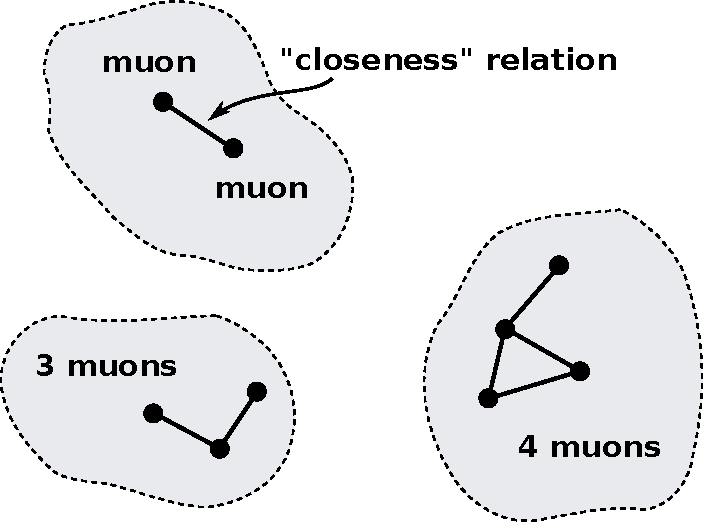
\includegraphics[width=\linewidth]{closeness.pdf}
\column{0.5\linewidth}
Muons are grouped if
\begin{itemize}
\item they are ``close'' to each other
\item they're close to another muon which is close to another, etc.
\end{itemize}

No dependence on the order of the grouping process, easy to analyze
\end{columns}

\begin{itemize}
\item Definition of ``closeness'' is tunable, with these ingredients:
\begin{itemize}\setlength{\itemsep}{0.1 cm}
\item $\Delta R$: geometrically close in a metric with uniform background
\item $m_\s{inv}$: guarantees that low-mass objects will be found, regardless of boost
\item $P_\s{vertex}$: requires a consistent track vertex
\item opposite charge: avoids connecting groups that can't be from the same neutral resonance
\end{itemize}
\end{itemize}
\end{frame}

\begin{frame}
\frametitle{Merging muons into groups}

Grouping efficiency vs.\ reconstructed mass and $\Delta R$

(denominator: found two muons, numerator: grouped them)

\vfill
\begin{columns}
\column{0.7\linewidth}
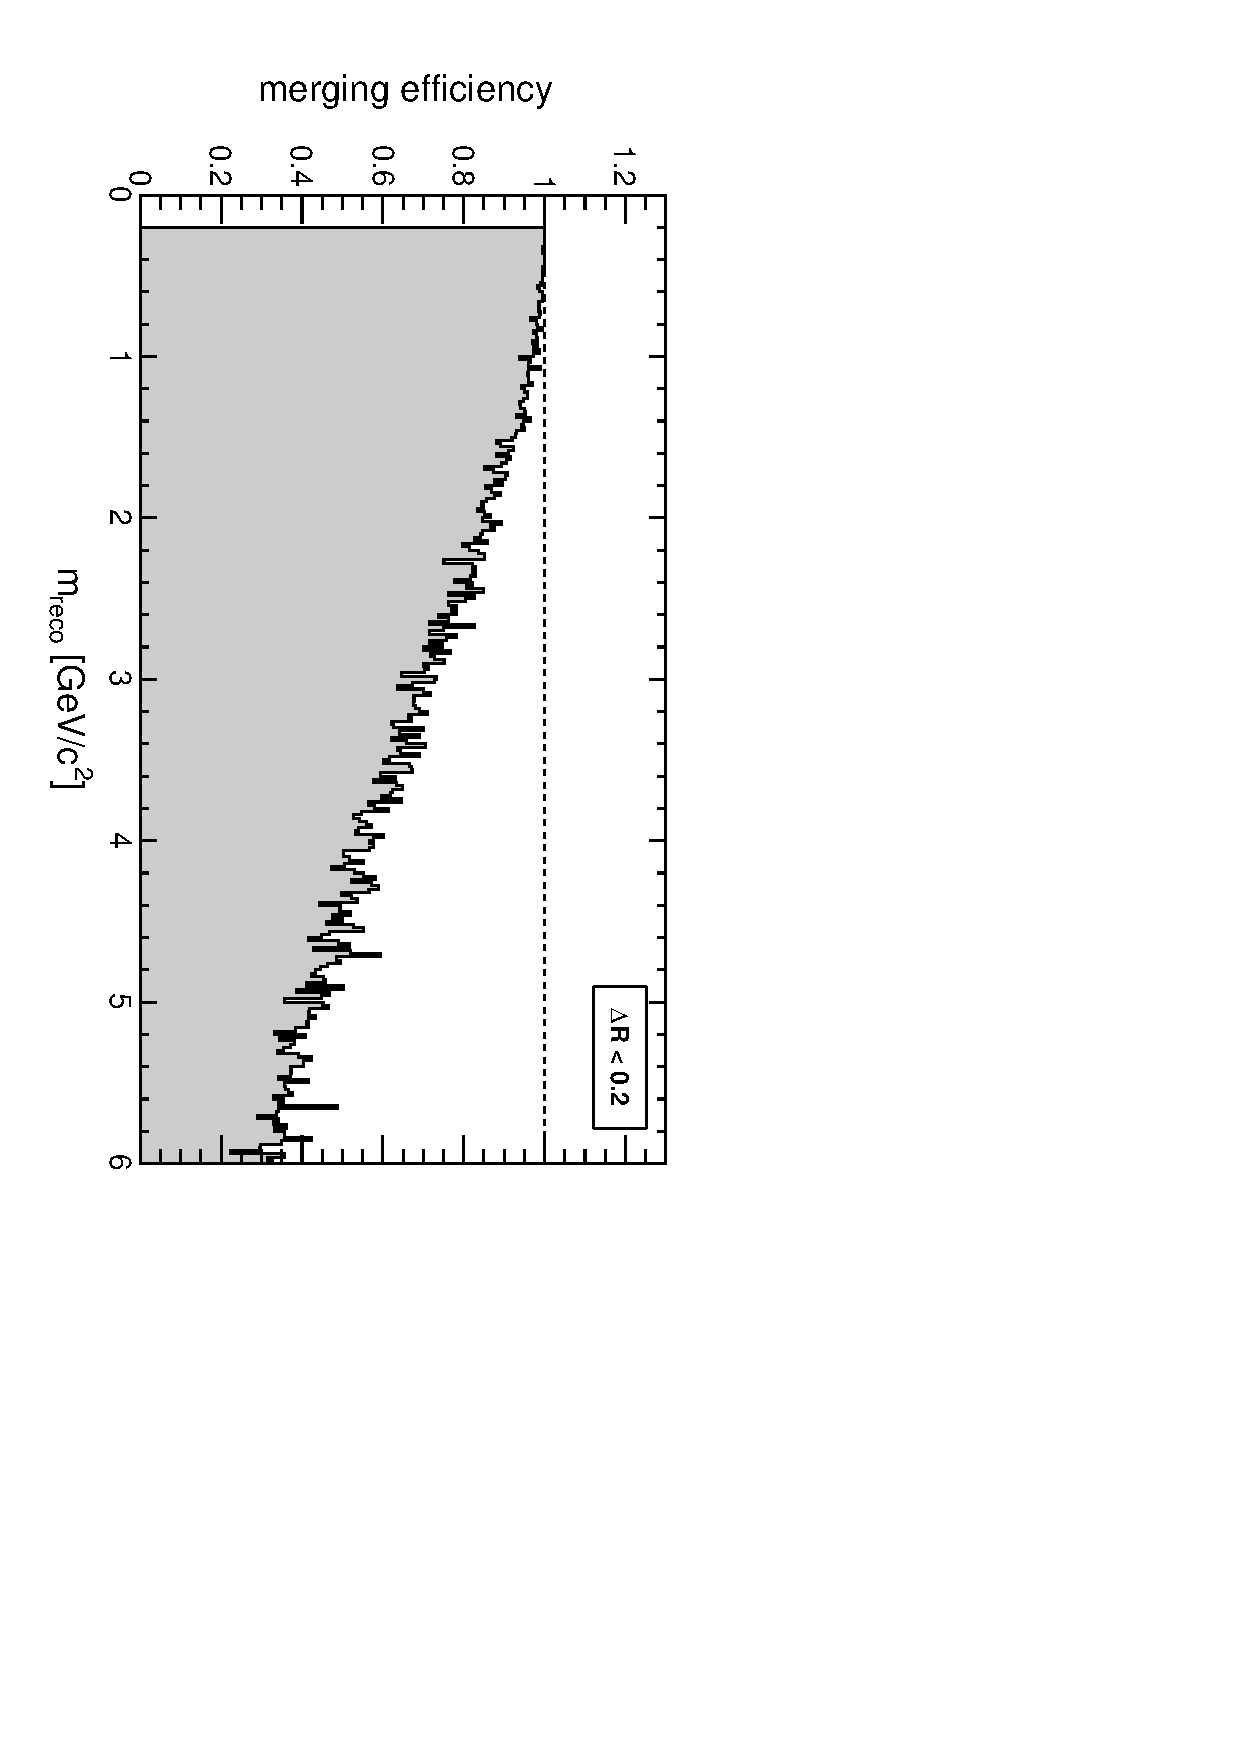
\includegraphics[height=0.5\linewidth, angle=90]{mergingeff_recomass_GroupByDeltaR.pdf}
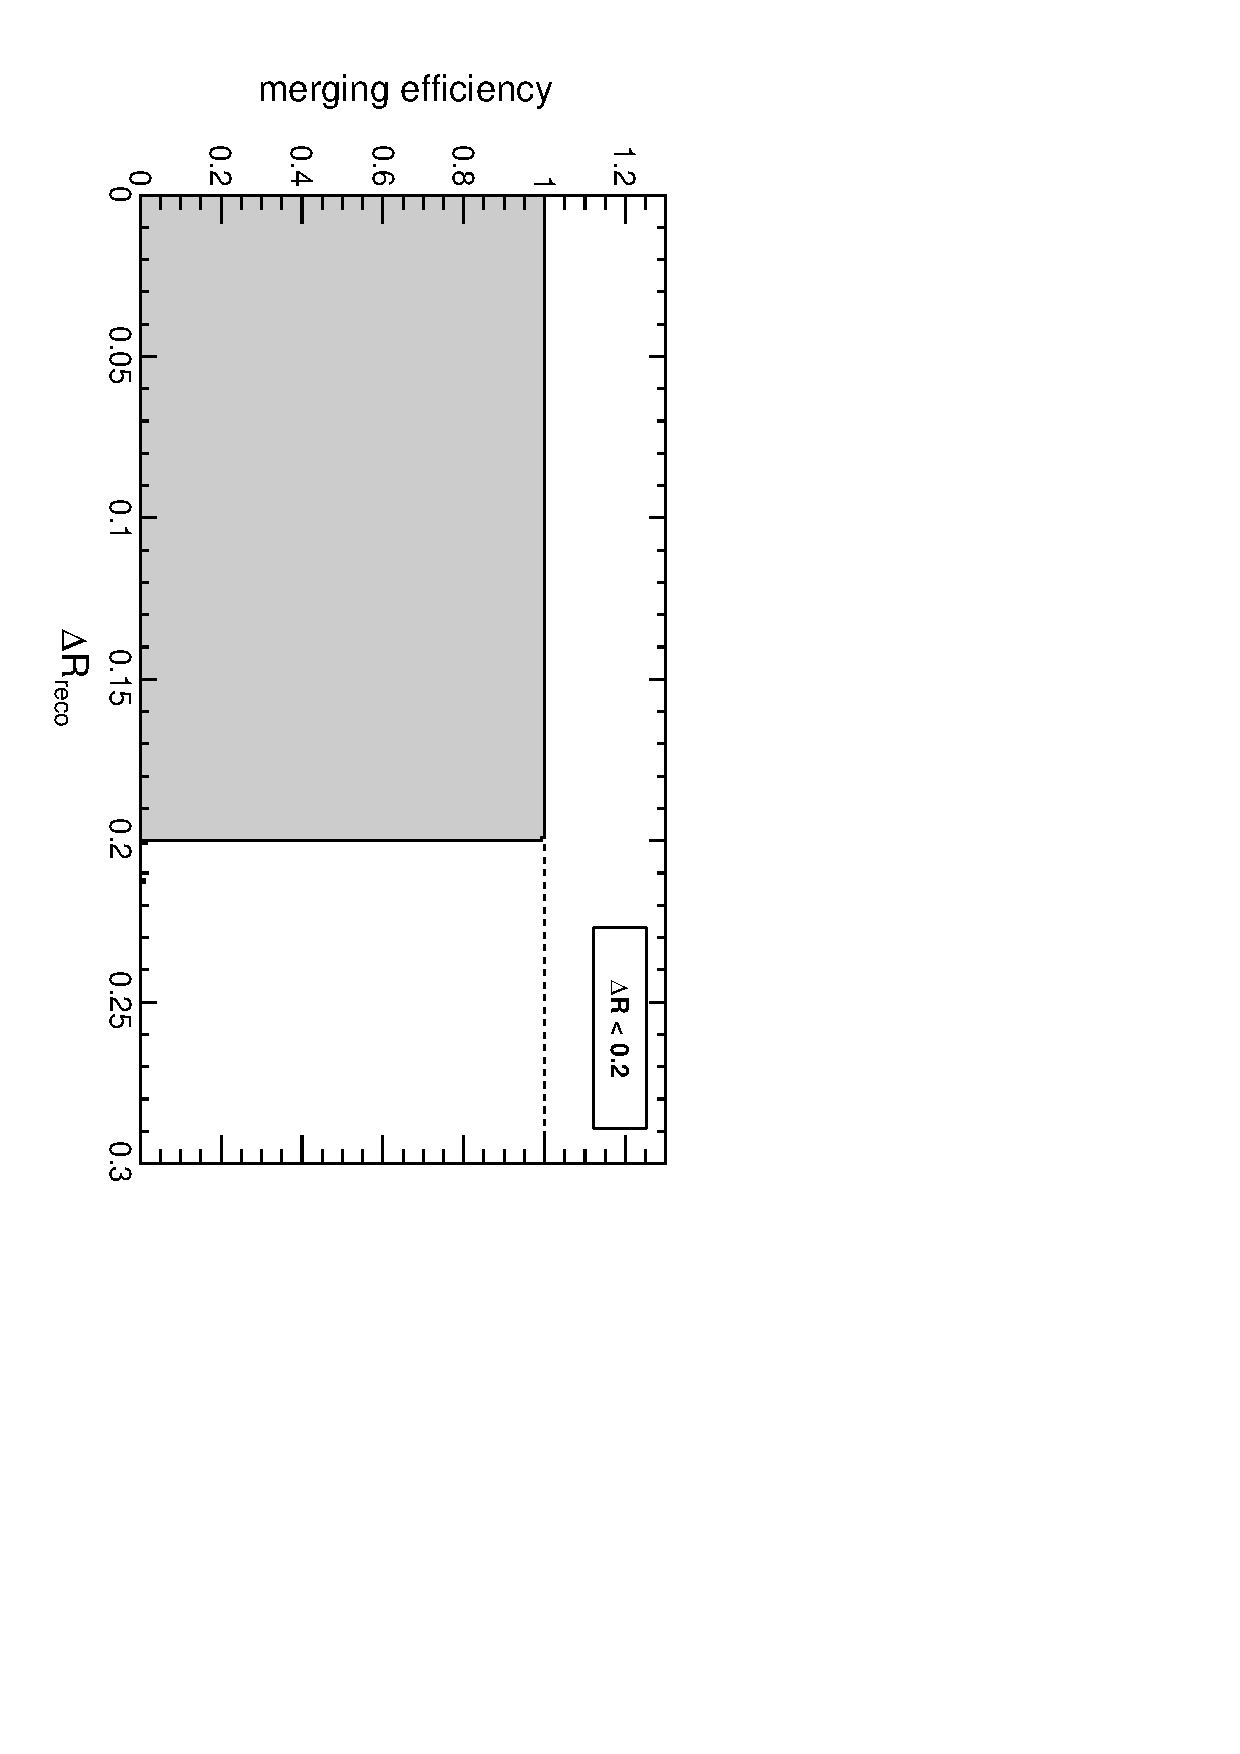
\includegraphics[height=0.5\linewidth, angle=90]{mergingeff_recodr_GroupByDeltaR.pdf}
\column{0.3\linewidth}
$\Delta R < 0.2$
\end{columns}

\begin{columns}
\column{0.7\linewidth}
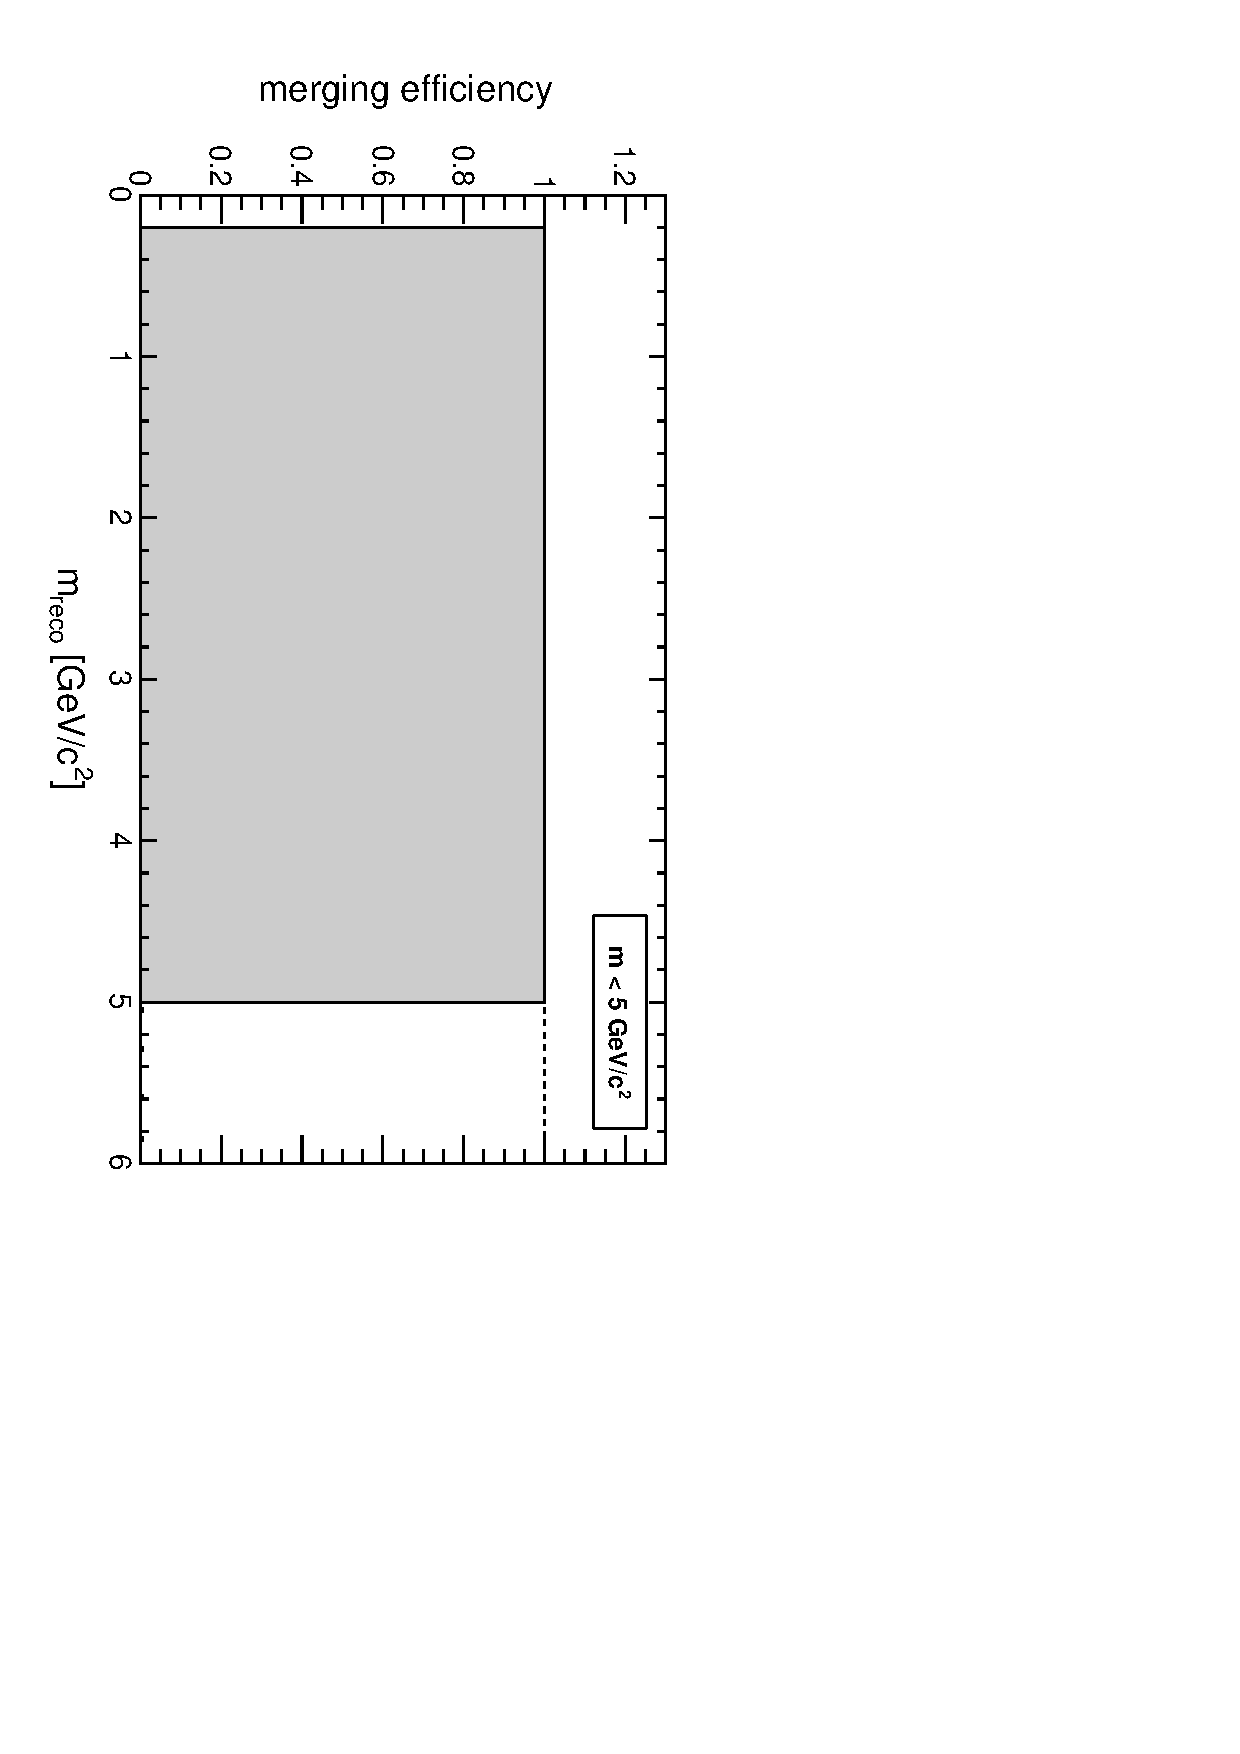
\includegraphics[height=0.5\linewidth, angle=90]{mergingeff_recomass_GroupByMass.pdf}
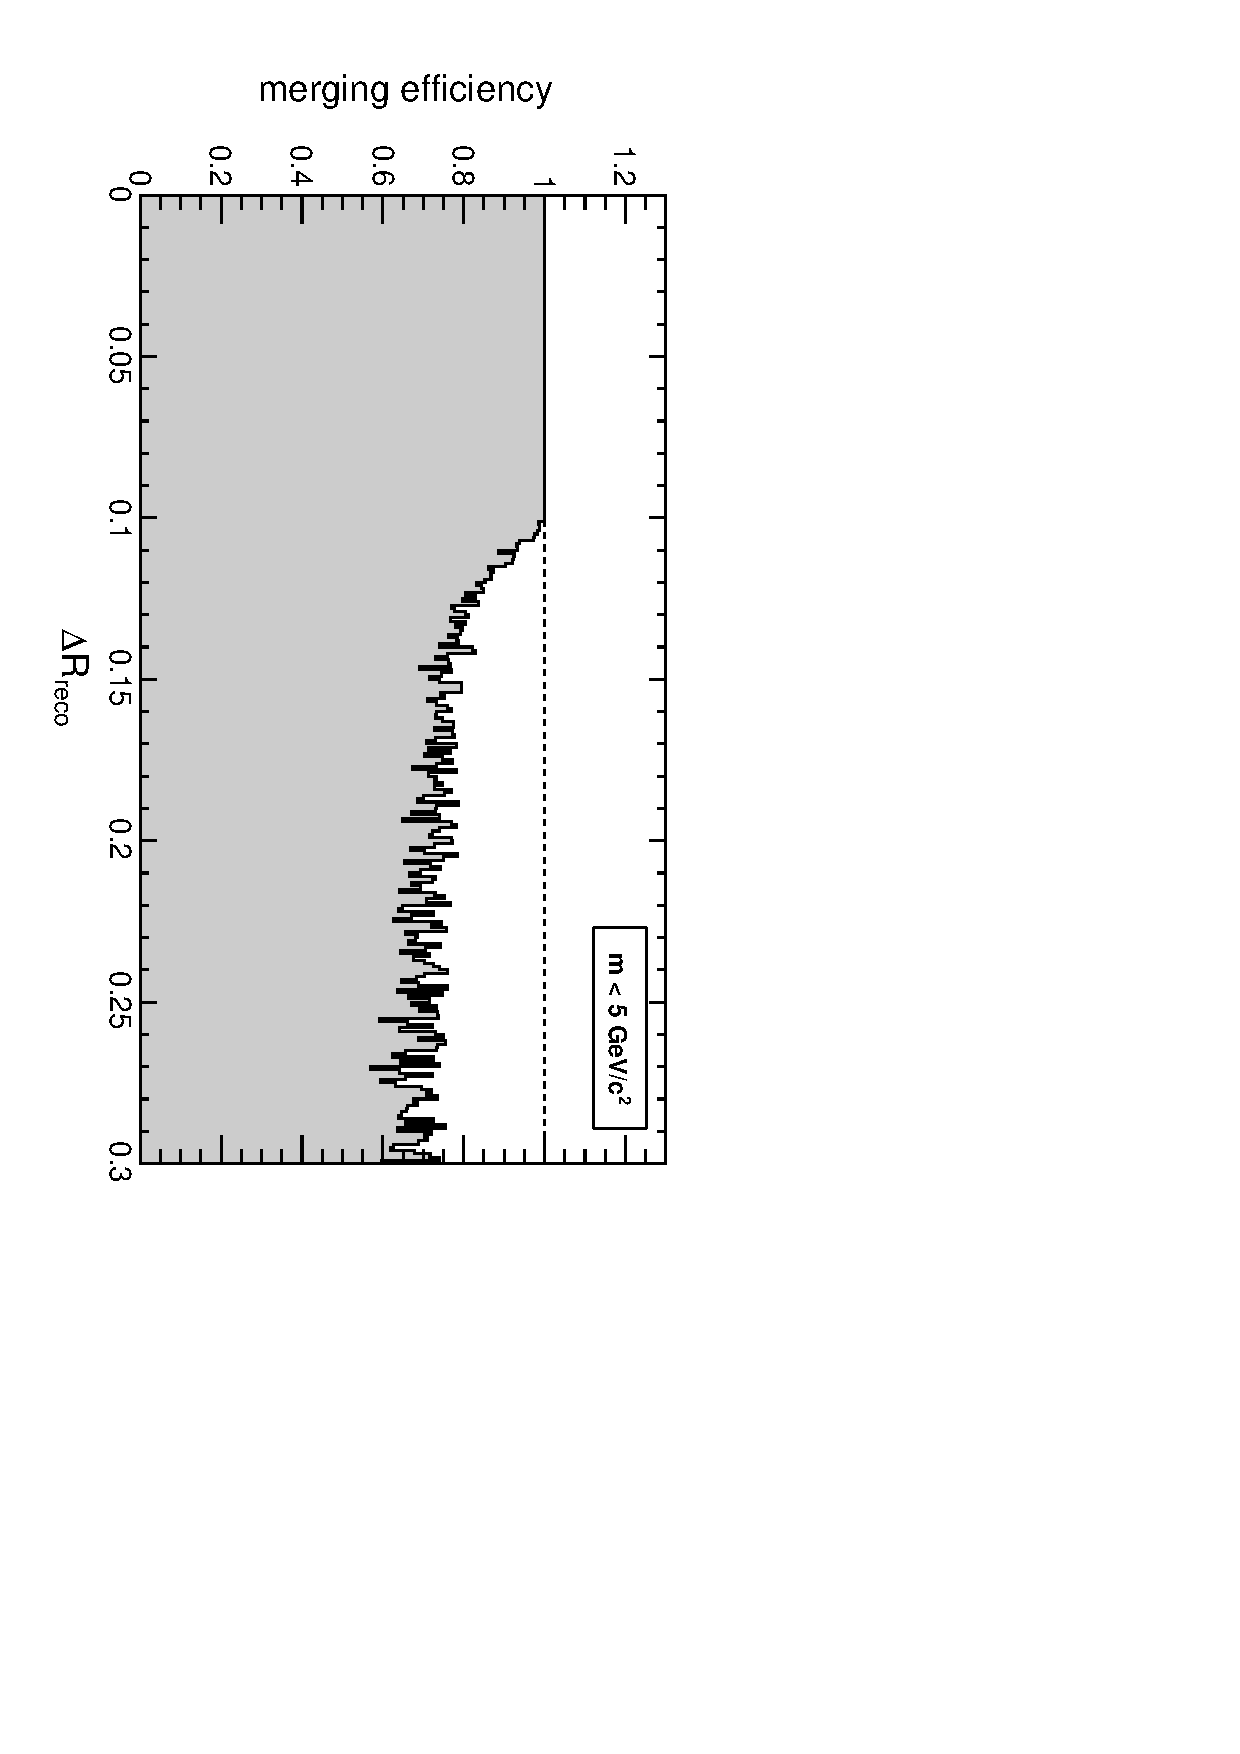
\includegraphics[height=0.5\linewidth, angle=90]{mergingeff_recodr_GroupByMass.pdf}
\column{0.3\linewidth}
$m_\s{inv} < 5$~GeV/$c$
\end{columns}

\begin{columns}
\column{0.7\linewidth}
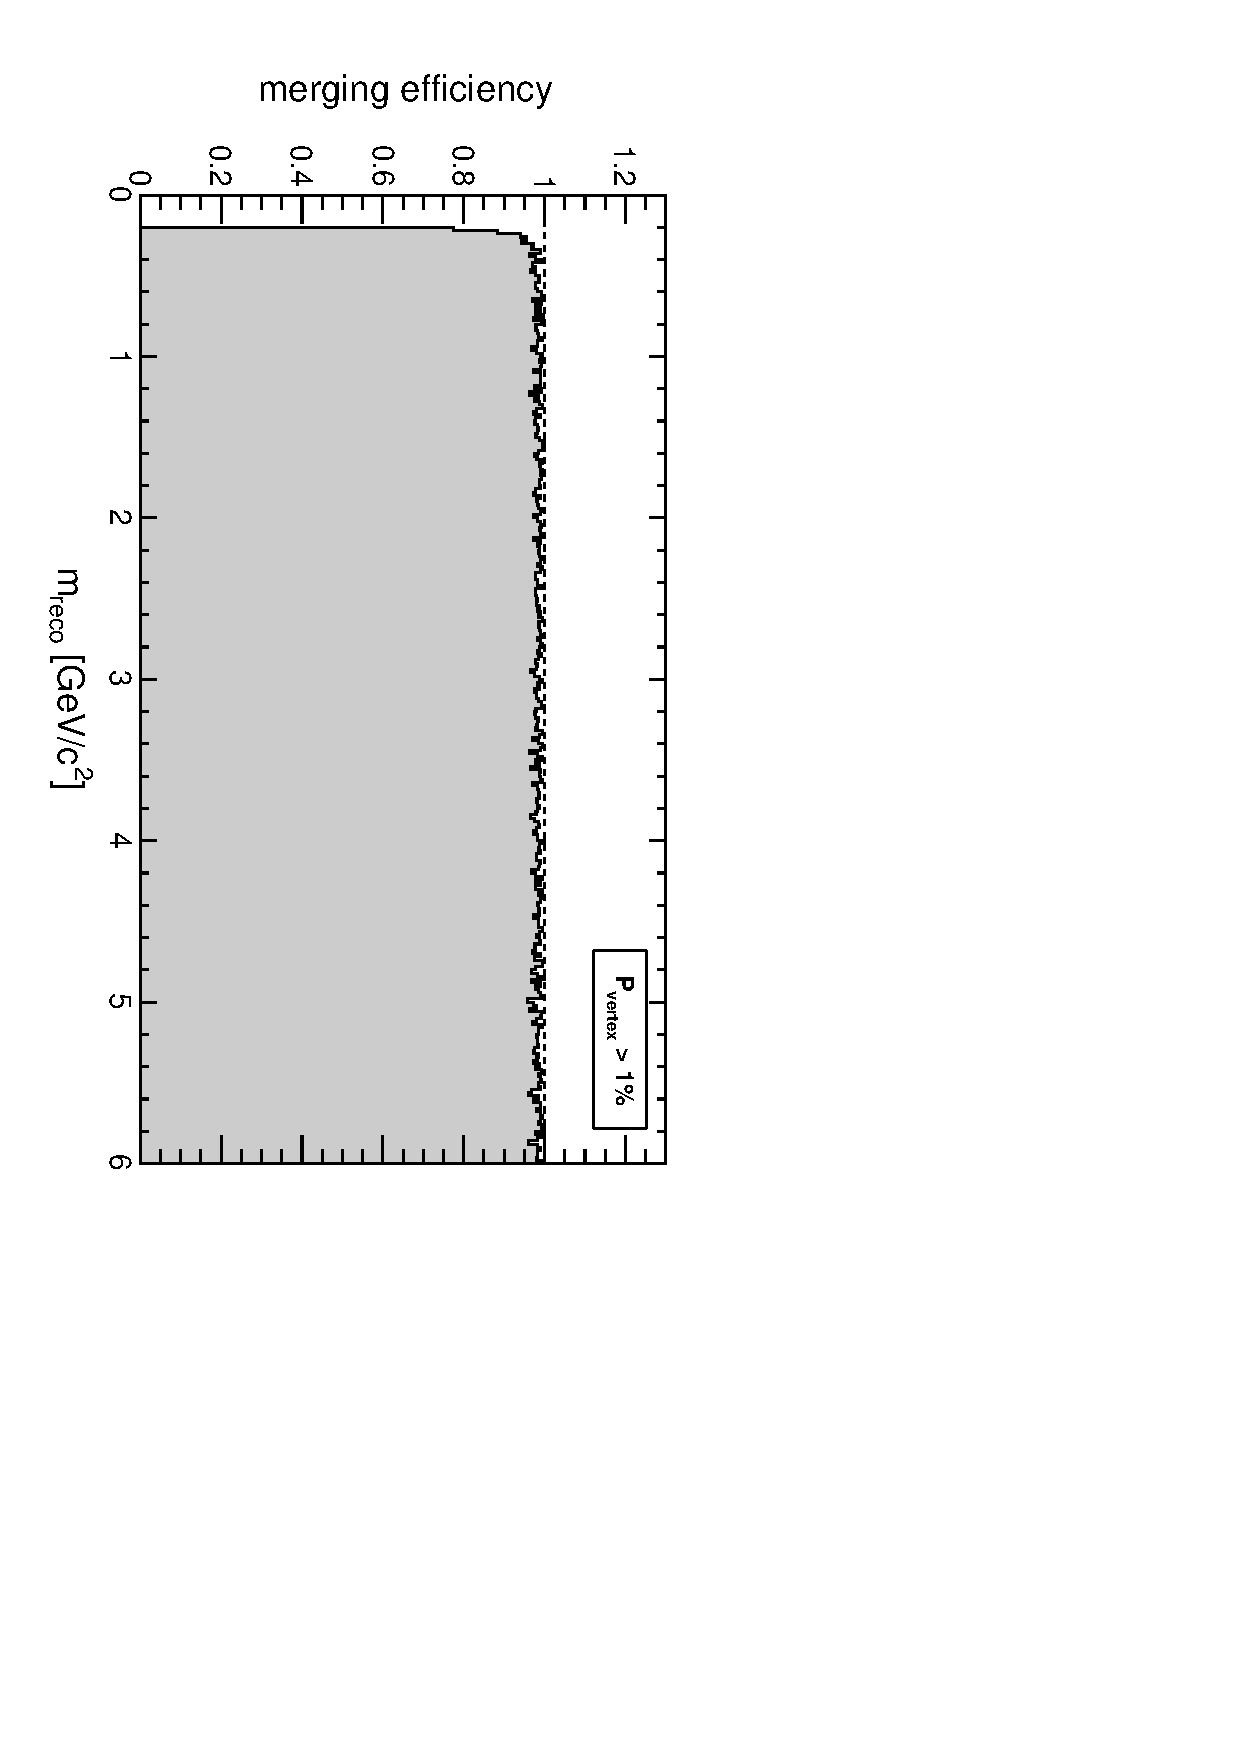
\includegraphics[height=0.5\linewidth, angle=90]{mergingeff_recomass_GroupByVertexProb.pdf}
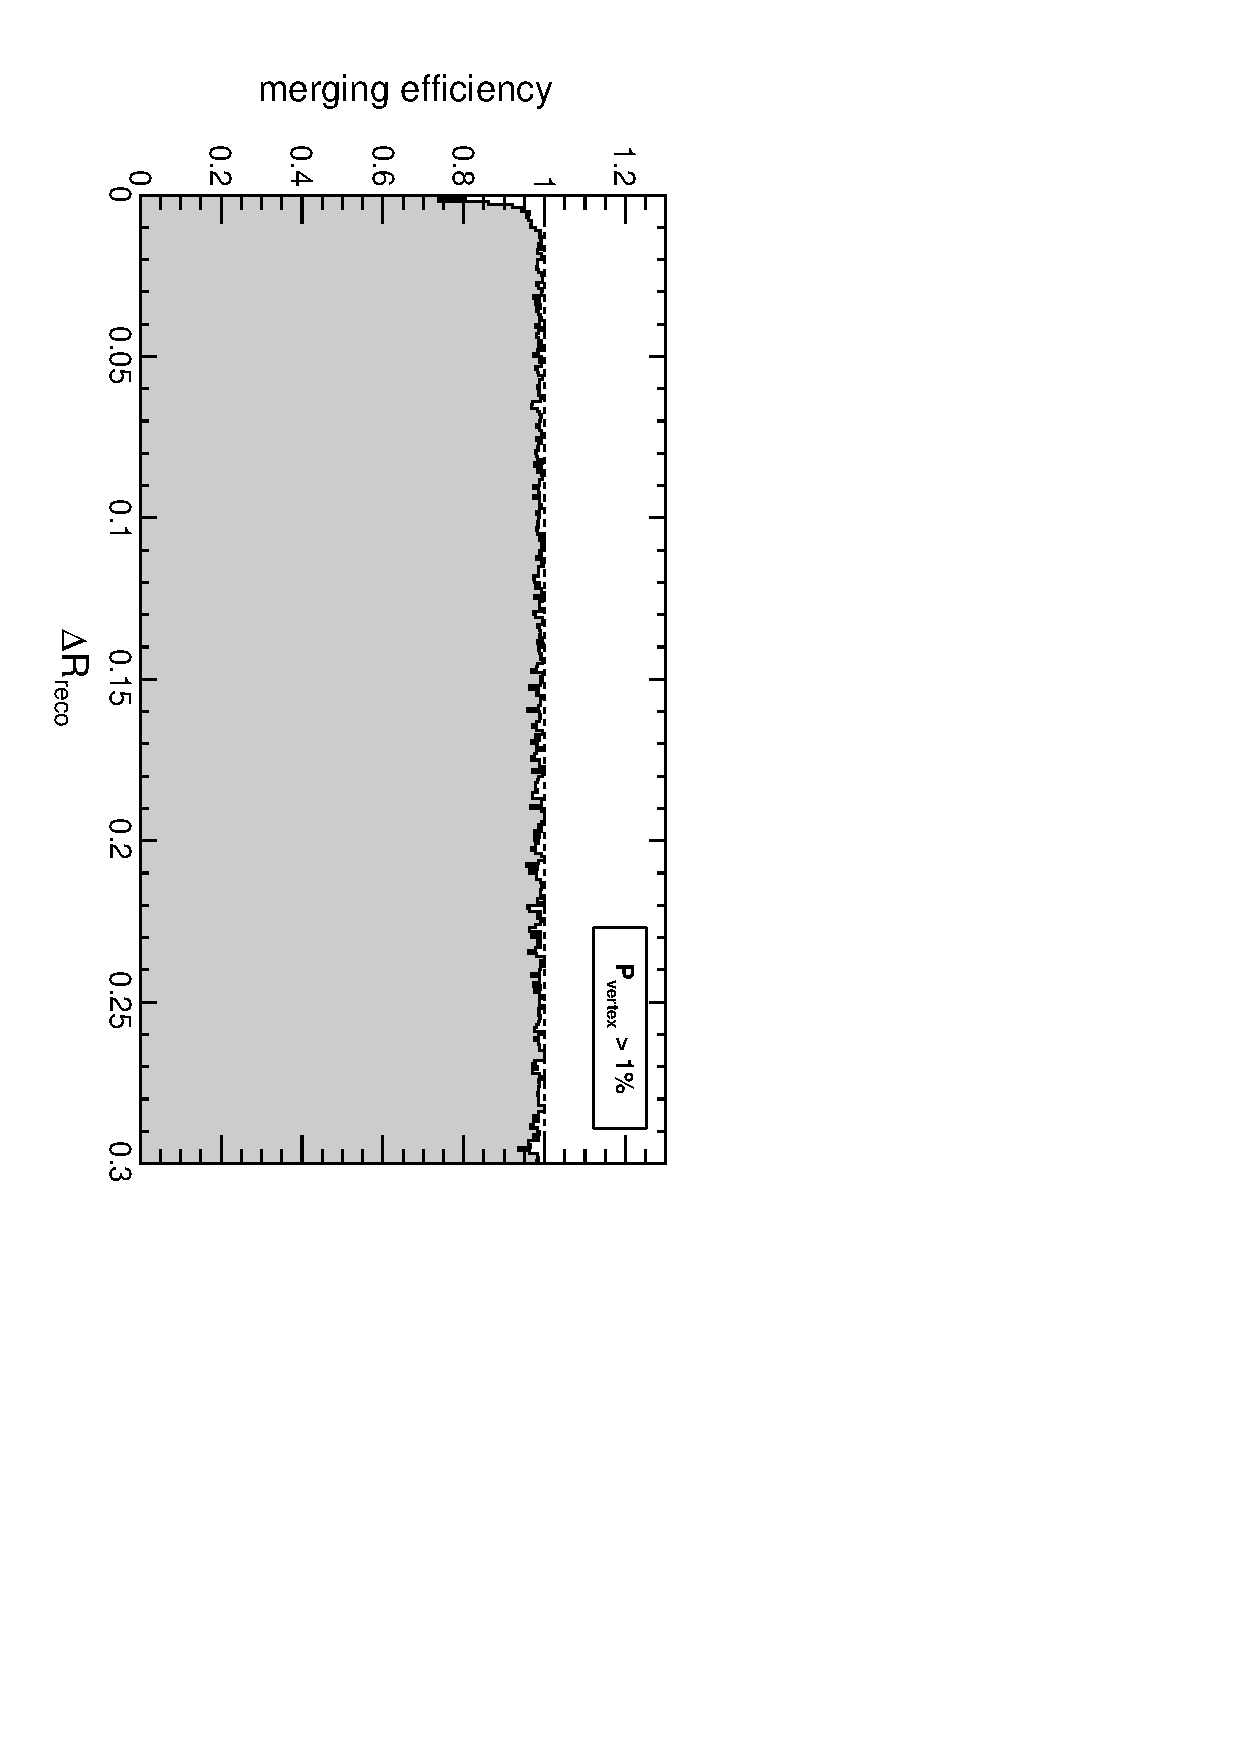
\includegraphics[height=0.5\linewidth, angle=90]{mergingeff_recodr_GroupByVertexProb.pdf}

\column{0.3\linewidth}
$P_\s{vertex} > 1$\%

\vspace{0.25 cm}
{\scriptsize (Note low efficiency due to vertexing failures for collinear muons)}
\end{columns}
\end{frame}

\begin{frame}
\frametitle{Merging muons into groups}
Optimization: group by
\begin{center}
$(m_{\mbox{\scriptsize inv}} < 5\mbox{ GeV/}c \mbox{\bf\mbox{ and }} P_{\mbox{\scriptsize vertex}} > 1\%) \mbox{\bf\mbox{ or }} \Delta R < 0.1$
\end{center}
\begin{itemize}
\item We guarantee that we get low-mass objects
\item Usually require them to vertex well
\item Except when they're very close together
\end{itemize}

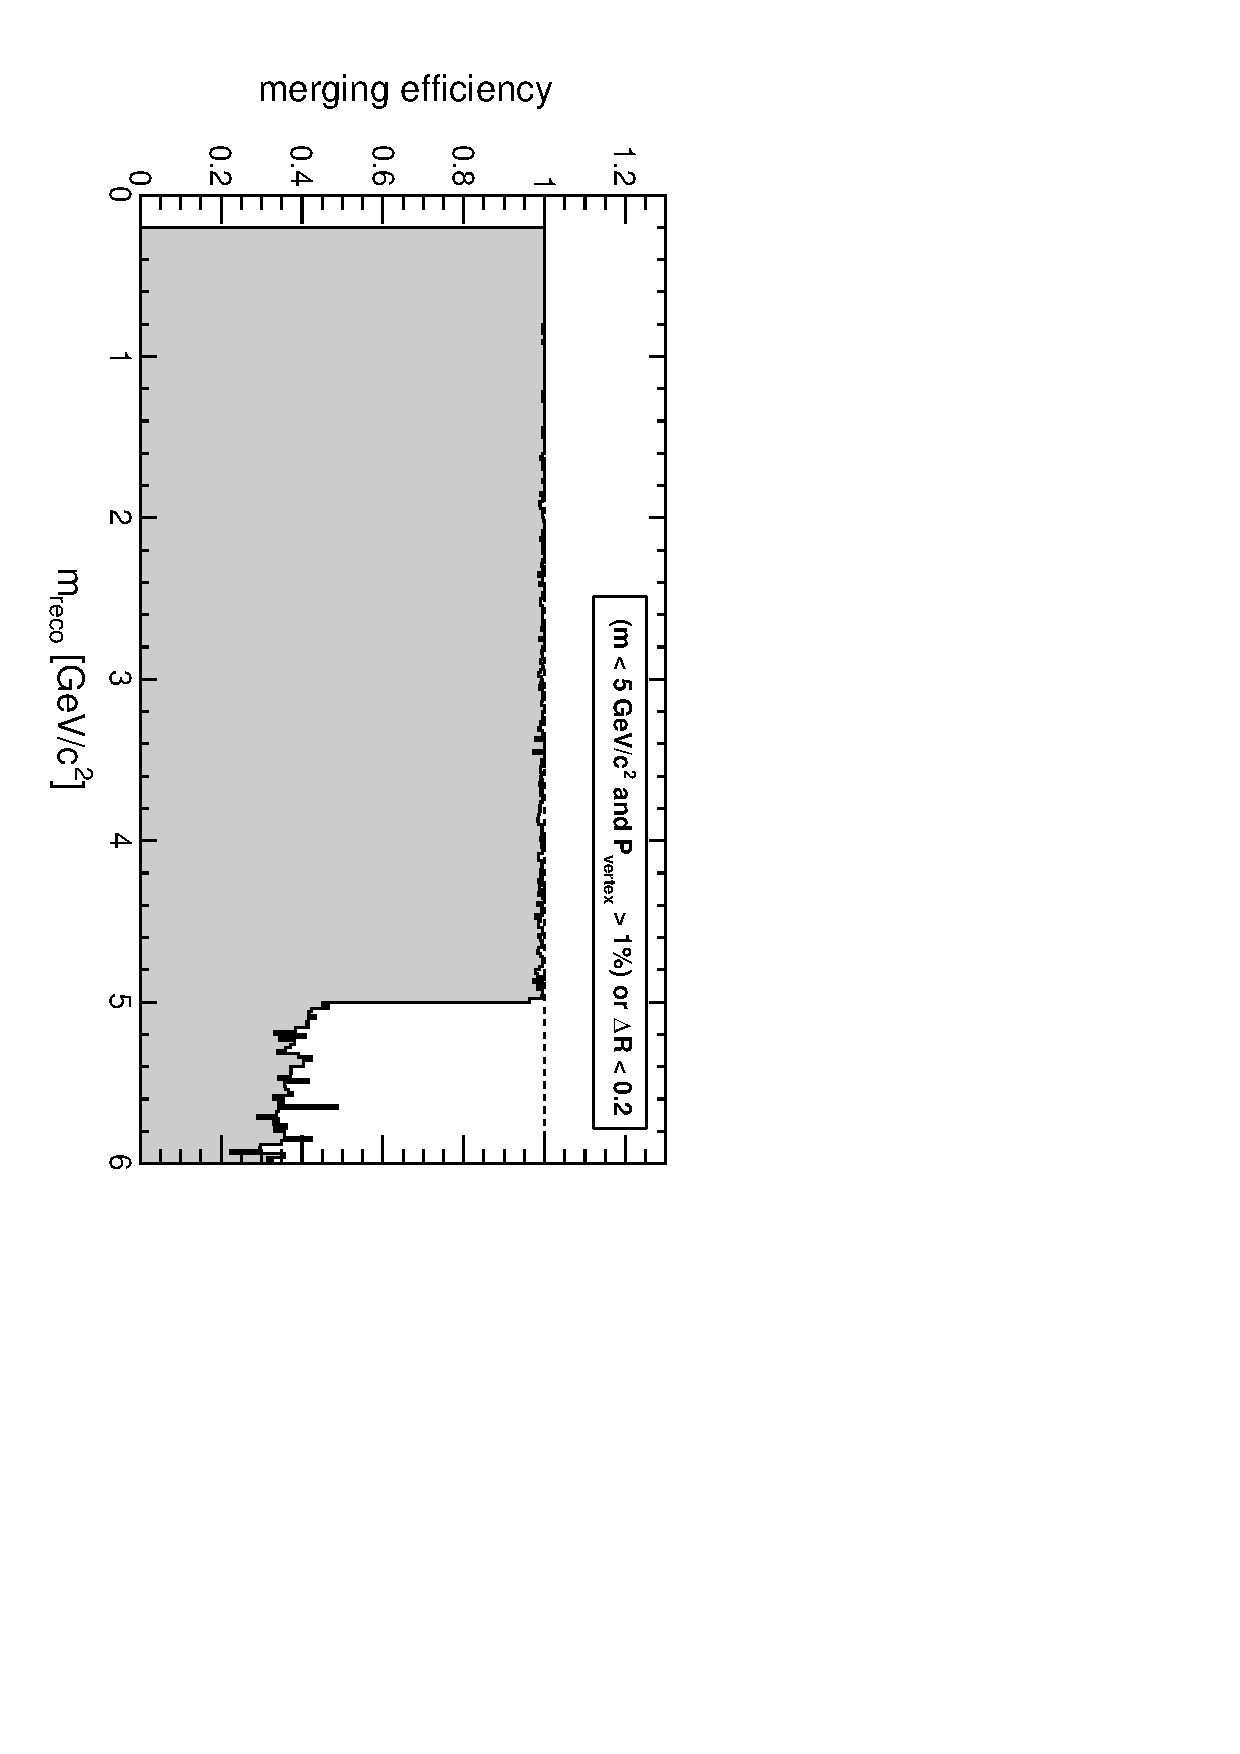
\includegraphics[height=0.5\linewidth, angle=90]{mergingeff_recomass_GroupByMassAndVertexProbOrDeltaR.pdf}
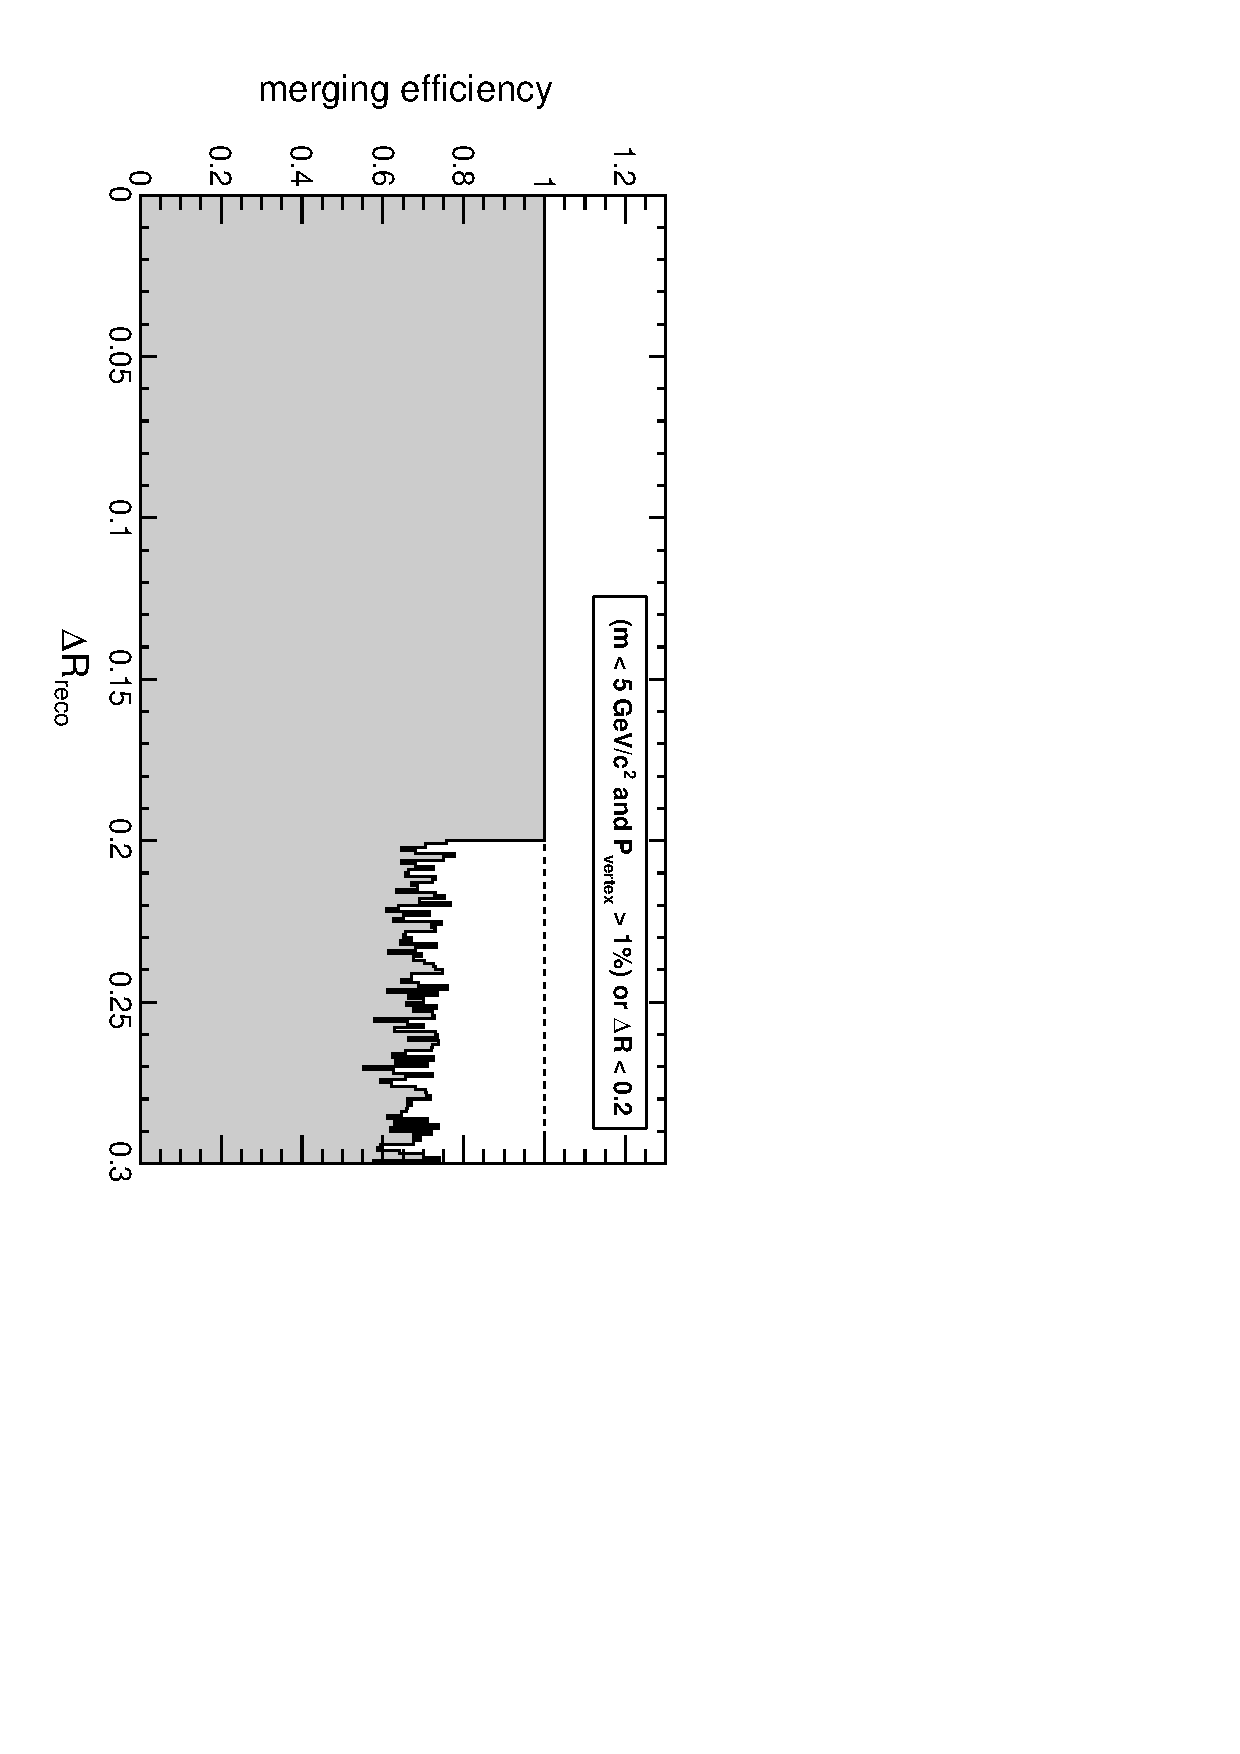
\includegraphics[height=0.5\linewidth, angle=90]{mergingeff_recodr_GroupByMassAndVertexProbOrDeltaR.pdf}

\vfill
Leave the opposite-sign requirement for later
\end{frame}

\begin{frame}
\frametitle{Merging muons into groups}

\begin{itemize}
\item If we have two low-mass ($m < 5$~GeV/$c^2$) dimuons in an event,
  what is the probability that they will be merged into two groups or one group?
\begin{itemize}\setlength{\itemsep}{0.1 cm}
\item $\alpha_\s{pair-pair}$ is the 3D angle between dimuons
\item $m_\s{pair-pair}$ is the parent particle mass
\item ``crossed'' means 1-2, 3-4 gets reconstructed as 1-3, 2-4
\end{itemize}

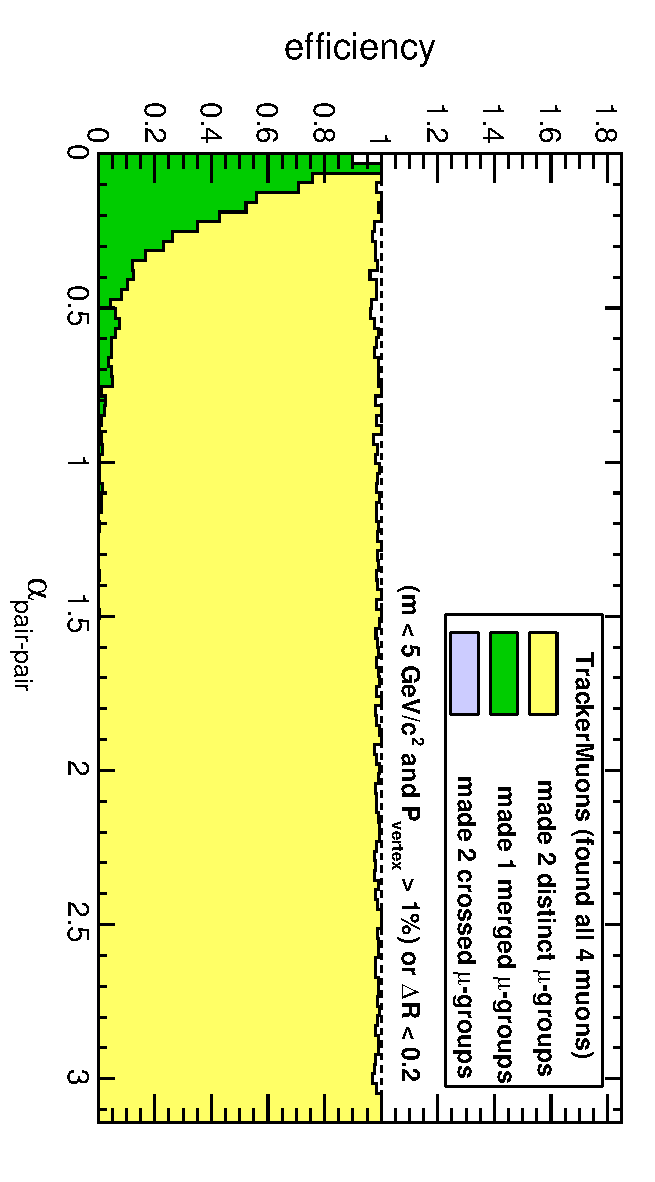
\includegraphics[height=0.5\linewidth, angle=90]{foundopening_TrackerMuonsGroupByMassAndVertexProbOrDeltaR.pdf}
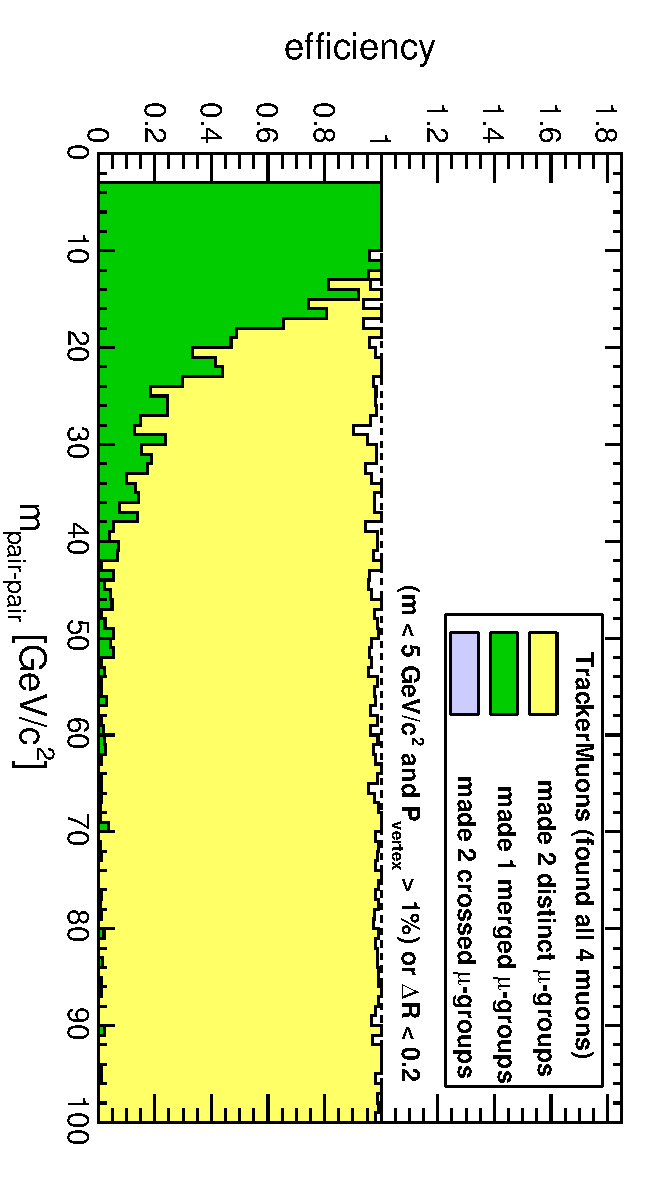
\includegraphics[height=0.5\linewidth, angle=90]{foundmass_TrackerMuonsGroupByMassAndVertexProbOrDeltaR.pdf}

\item Can be tuned with grouping criteria: loose ``closeness''
  criteria yield higher efficiency for pairs and higher probability
  of pair-merging
\item The plots above came from a flat-generated pair-pair gun; should
  try with realistic cascades because it could depend on kinematics
\end{itemize}
\end{frame}

\begin{frame}
\frametitle{Extra muons in group}

\begin{itemize}
\item $\mu$-groups can absorb an extra muon from unrelated \mbox{tracks in the event\hspace{-1 cm}}
\item Below: simulations with increasing amounts of pile-up ($\frac{N_\s{extra}}{N_\s{total}}$ vs.\ $\eta$)

left: TrackerMuon-groups, right: GlobalMuon-groups
\end{itemize}

\begin{columns}
\column{0.7\linewidth}
\mbox{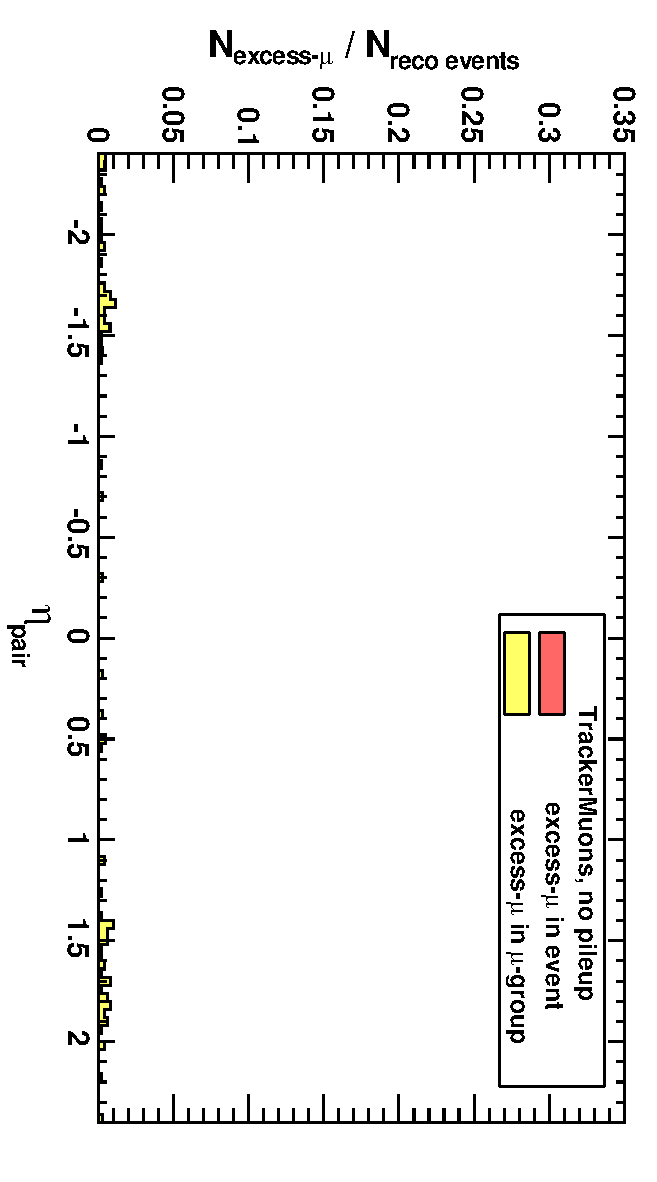
\includegraphics[height=0.5\linewidth, angle=90]{toomanymuons_TrackerMuonsGroupByMassAndVertexProbOrDeltaR.pdf}
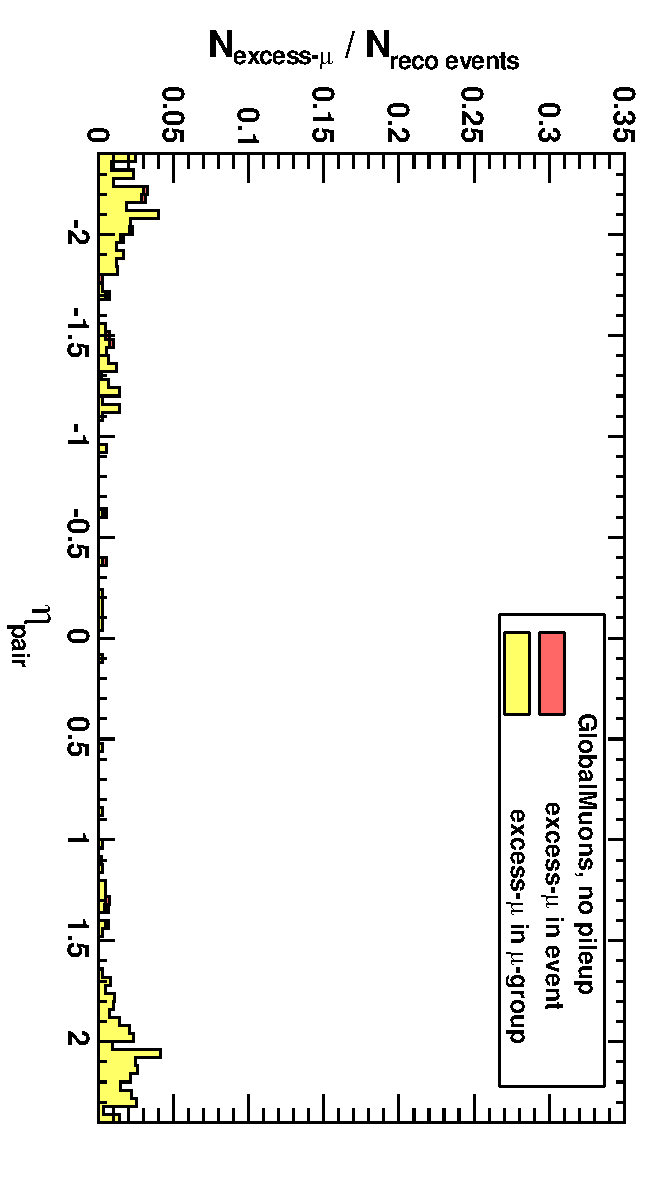
\includegraphics[height=0.5\linewidth, angle=90]{toomanymuons_GlobalMuonsGroupByMassAndVertexProbOrDeltaR.pdf}}

\mbox{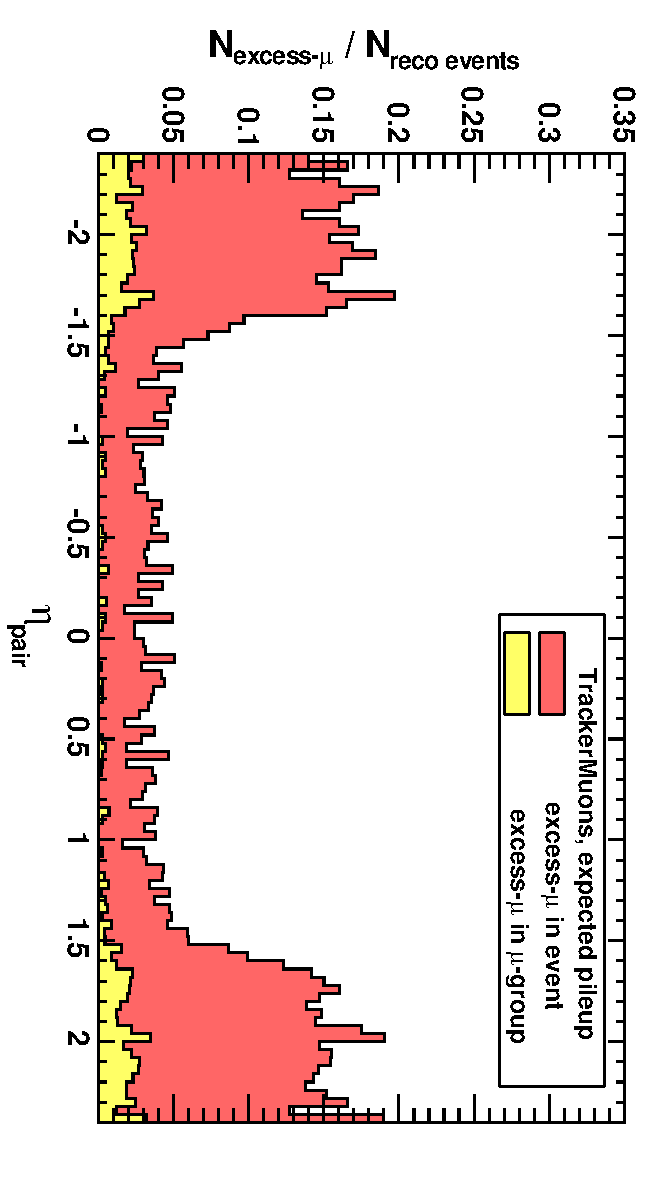
\includegraphics[height=0.5\linewidth, angle=90]{toomanymuons_TrackerMuonsGroupByMassAndVertexProbOrDeltaR_pileup.pdf}
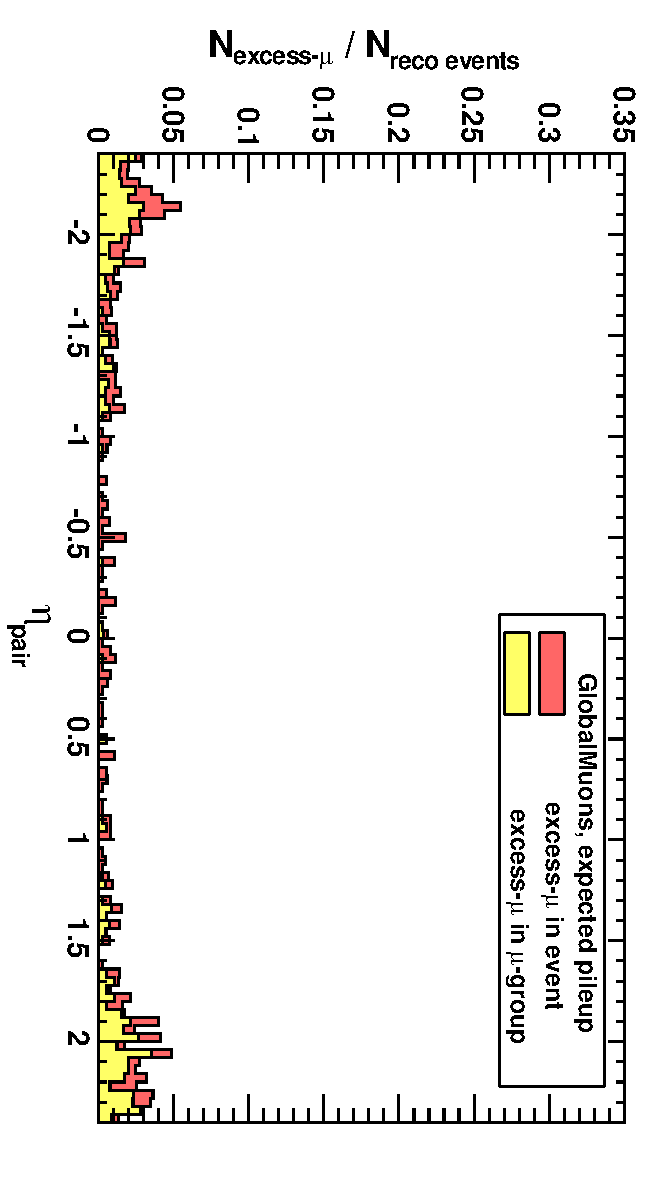
\includegraphics[height=0.5\linewidth, angle=90]{toomanymuons_GlobalMuonsGroupByMassAndVertexProbOrDeltaR_pileup.pdf}}

\mbox{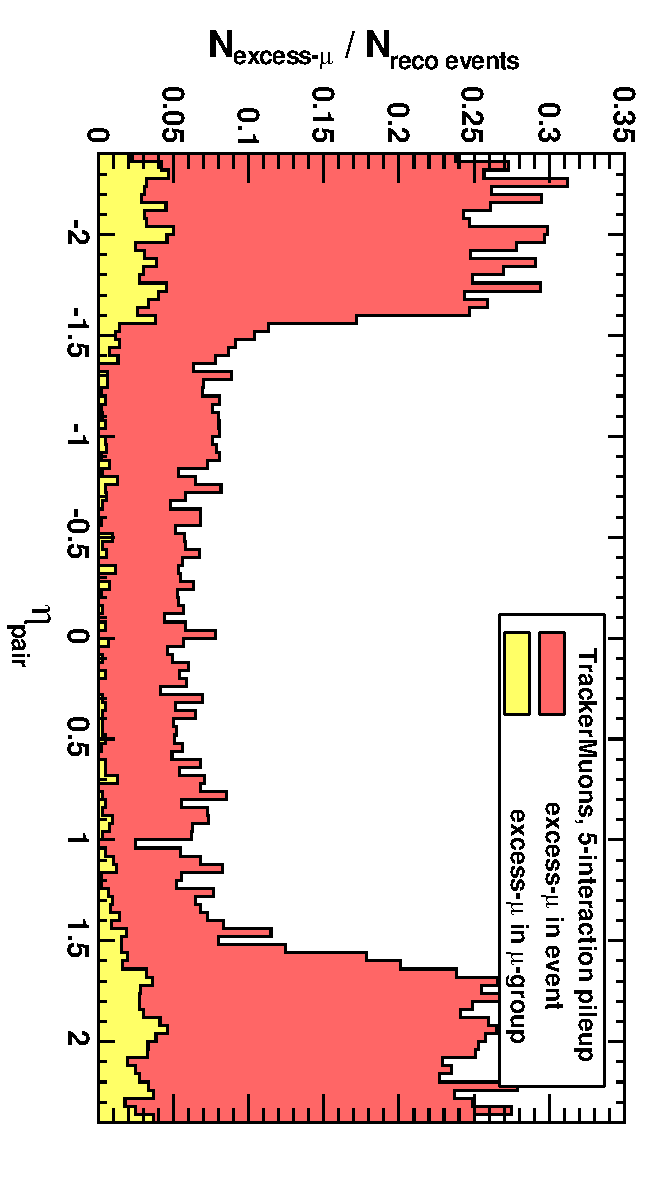
\includegraphics[height=0.5\linewidth, angle=90]{toomanymuons_TrackerMuonsGroupByMassAndVertexProbOrDeltaR_pileup5.pdf}
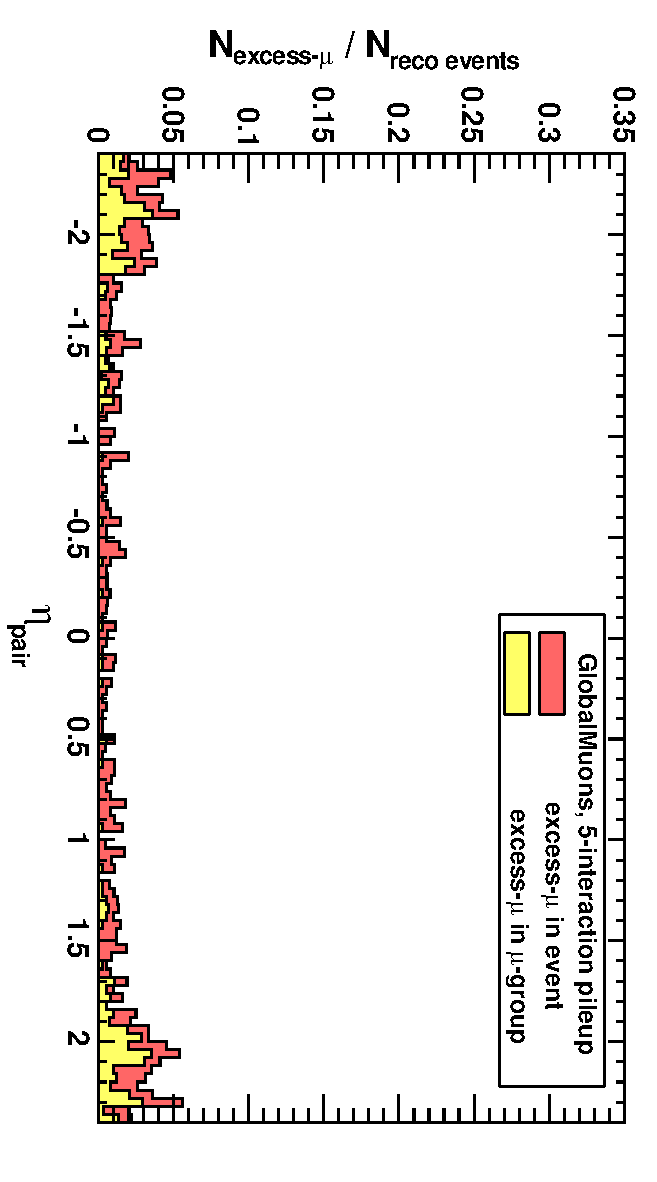
\includegraphics[height=0.5\linewidth, angle=90]{toomanymuons_GlobalMuonsGroupByMassAndVertexProbOrDeltaR_pileup5.pdf}}

\column{0.25\linewidth}
Despite extra tracks identified as muons (red), the extra-muons-in-group (yellow) is controlled by $P_\s{vertex} > 1\%$

\vspace{0.3 cm}
We'll also soon see that fake TrackerMuons can be controlled with quality cuts
\end{columns}
\end{frame}

\begin{frame}
\frametitle{Acceptance and efficiency}
\begin{itemize}
\item Acceptance region of a dimuon defined by $pT_2 > 5$~GeV/$c$ and
  $|\eta_1| < 2.4$ where $pT_2$ is the second-highest $p_T$ muon and
  $\eta_1$ is the highest-$|\eta|$ muon in the event
\item Try reconstructing muons in four different ways: TrackerMuons,
  StandAloneMuons, StandAlone-SET algorithm, and GlobalMuons

\end{itemize}
\begin{center}
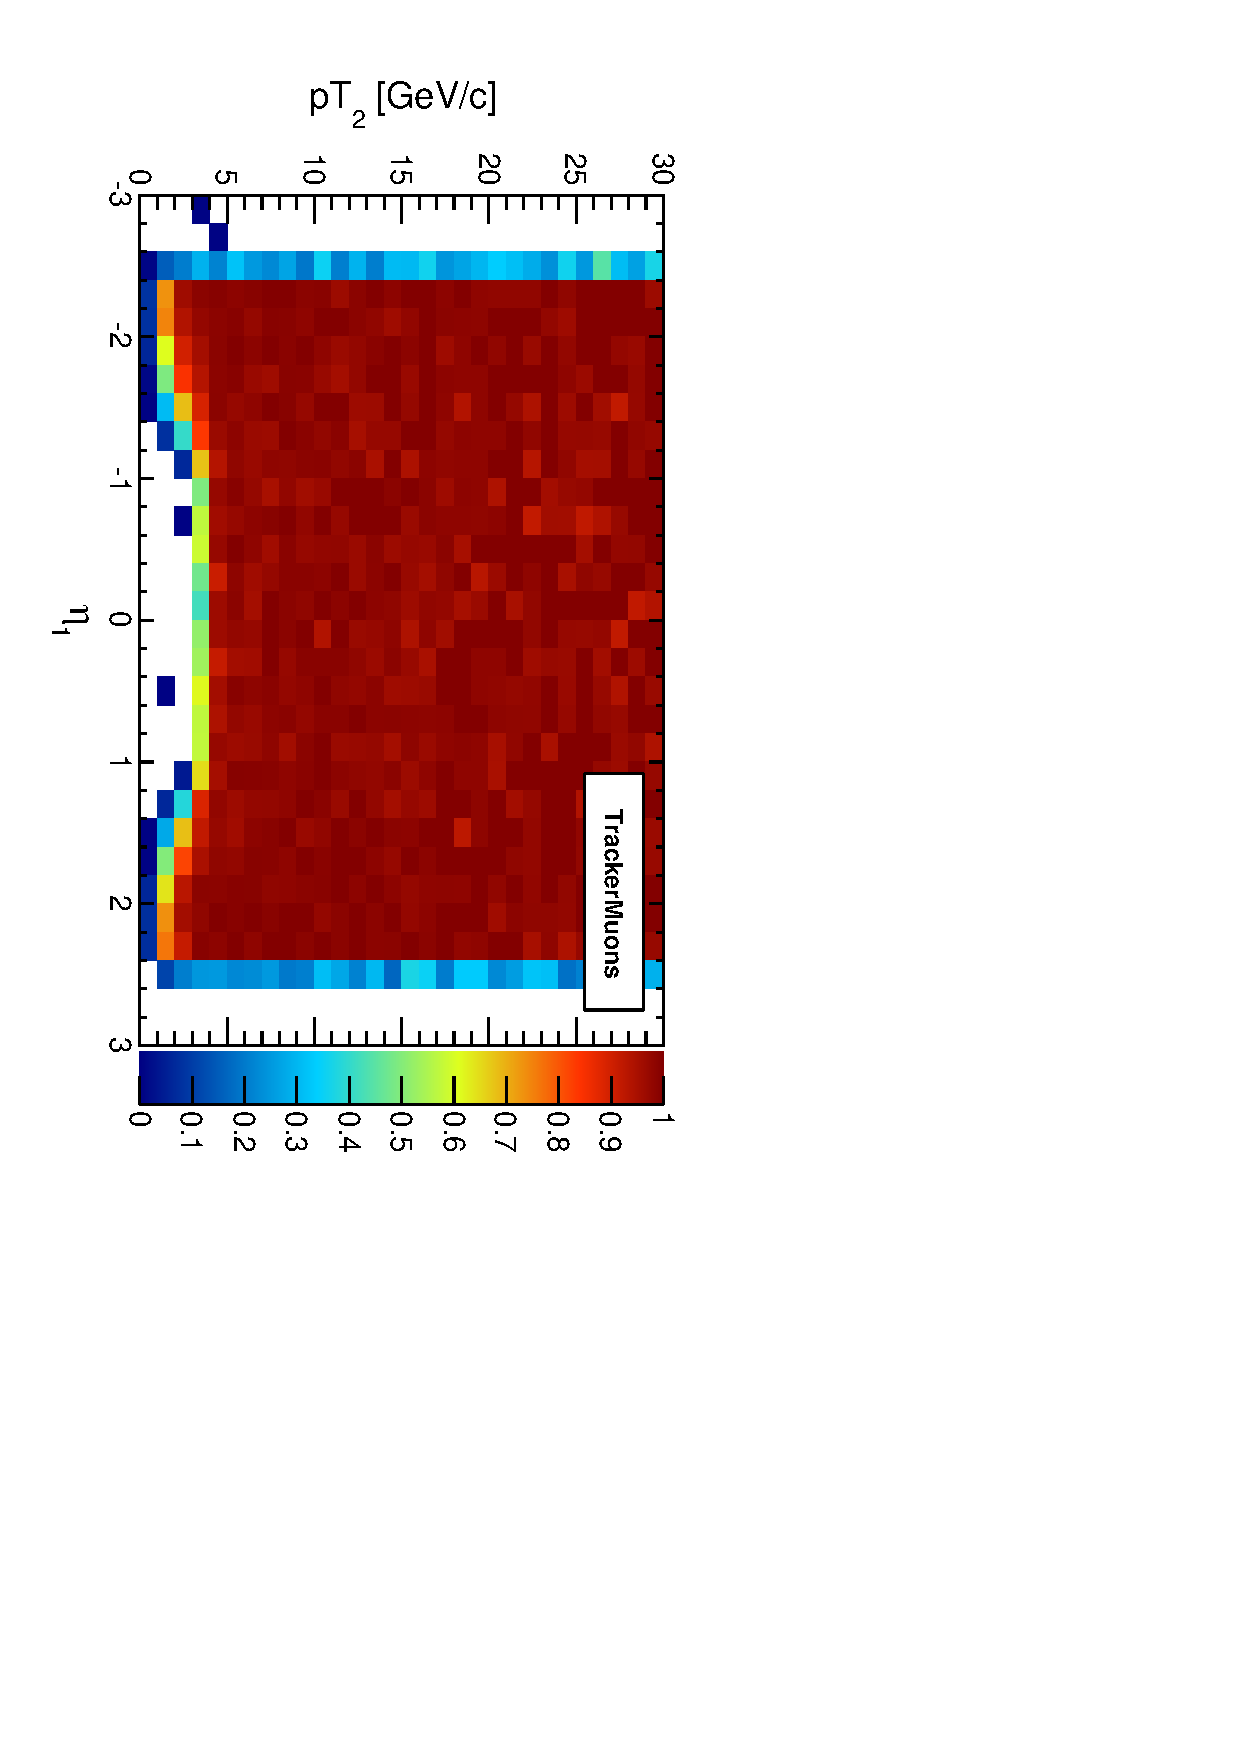
\includegraphics[height=0.45\linewidth, angle=90]{pt2vseta1_TrackerMuons.pdf}
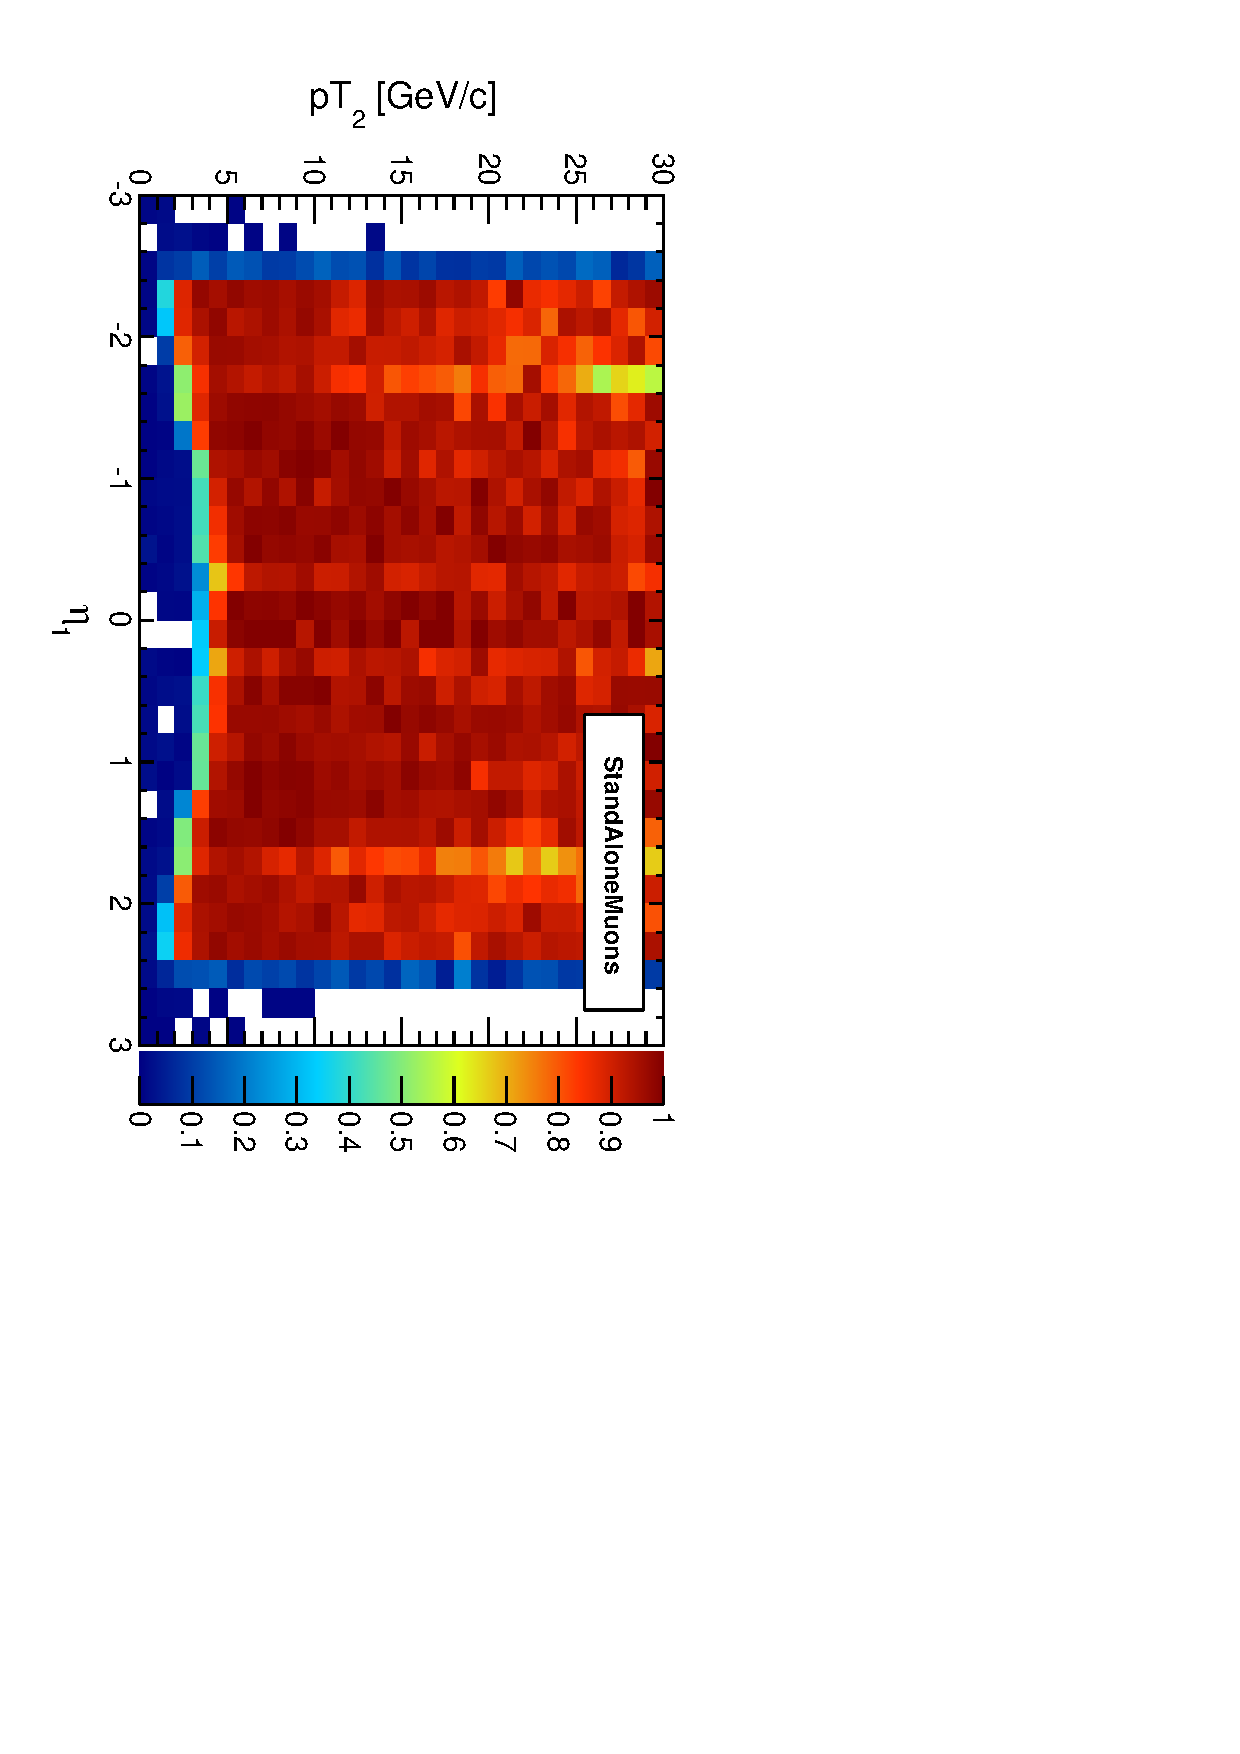
\includegraphics[height=0.45\linewidth, angle=90]{pt2vseta1_StandAloneUpdatedDefault.pdf}

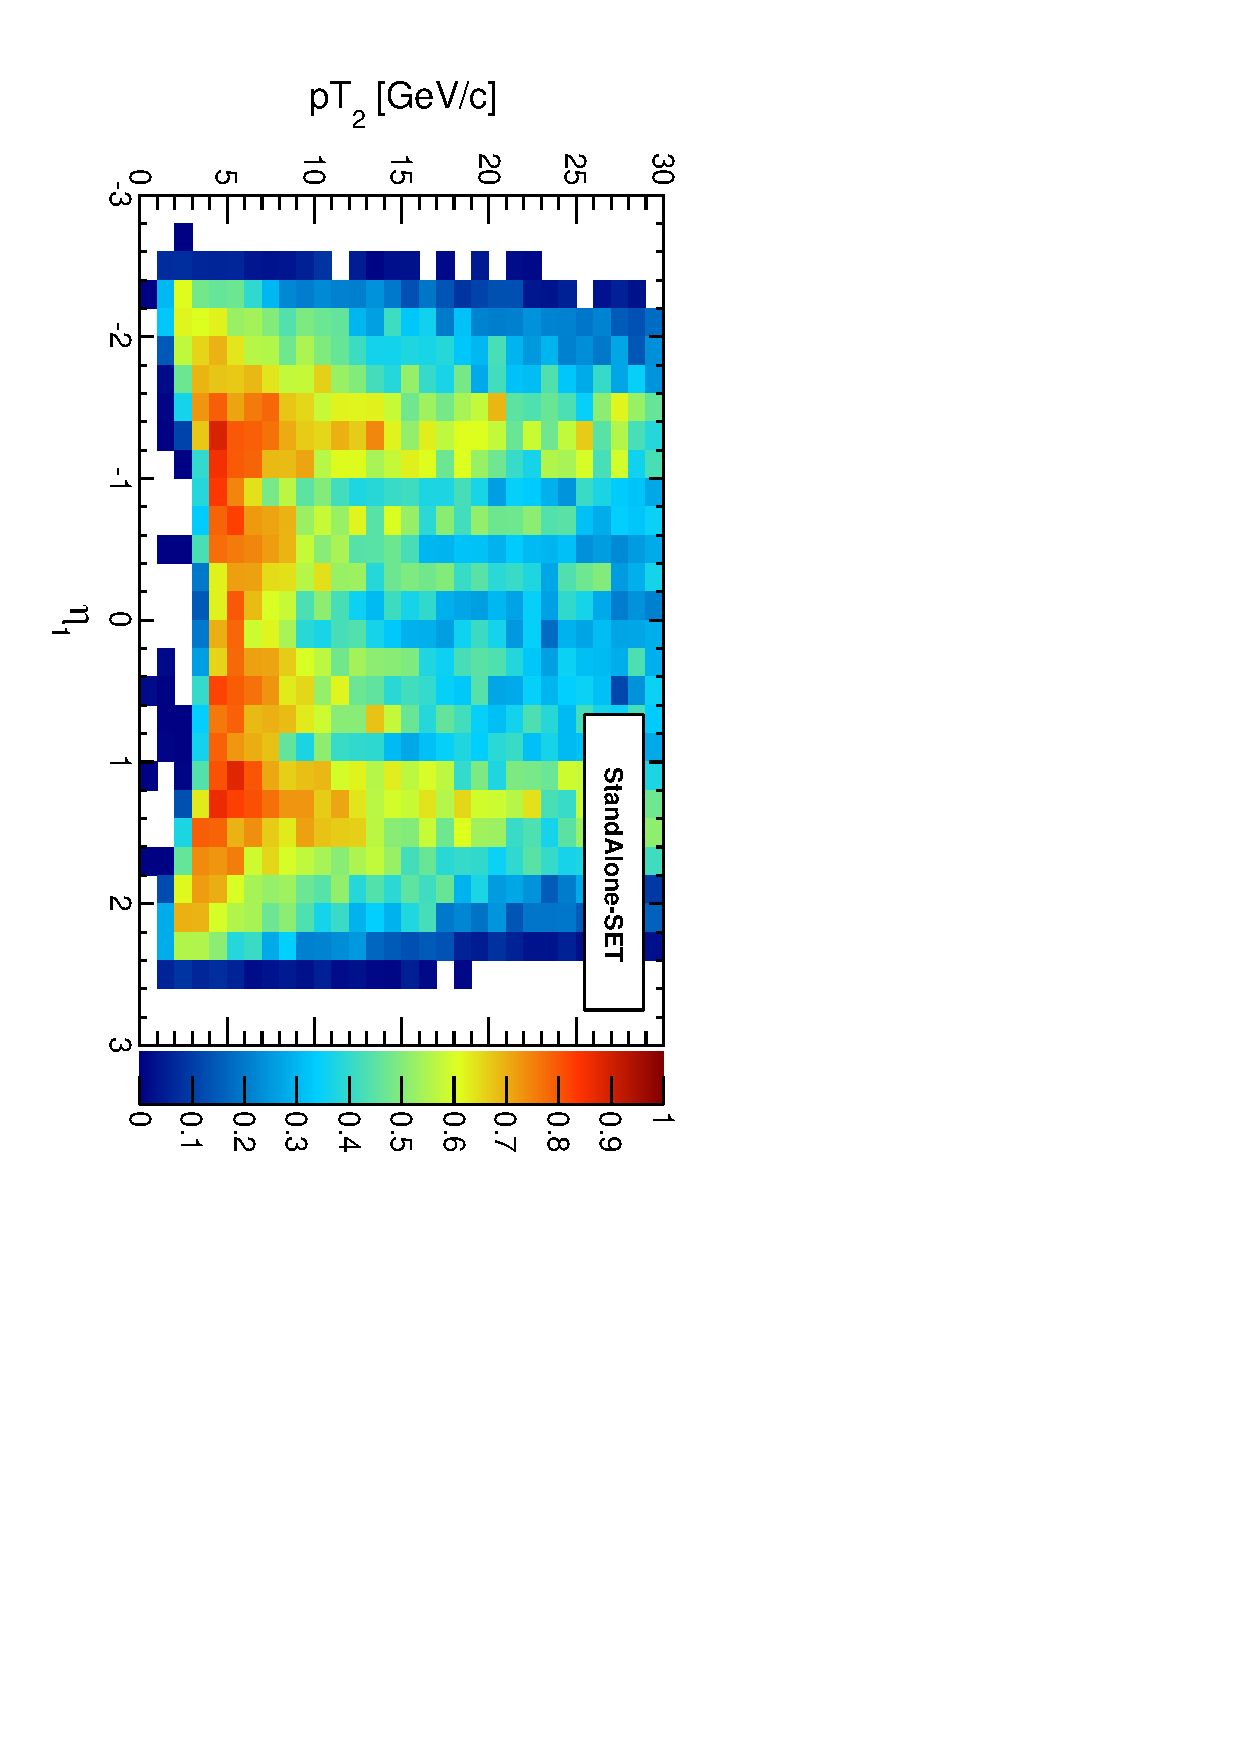
\includegraphics[height=0.45\linewidth, angle=90]{pt2vseta1_StandAloneUpdatedSET.pdf}
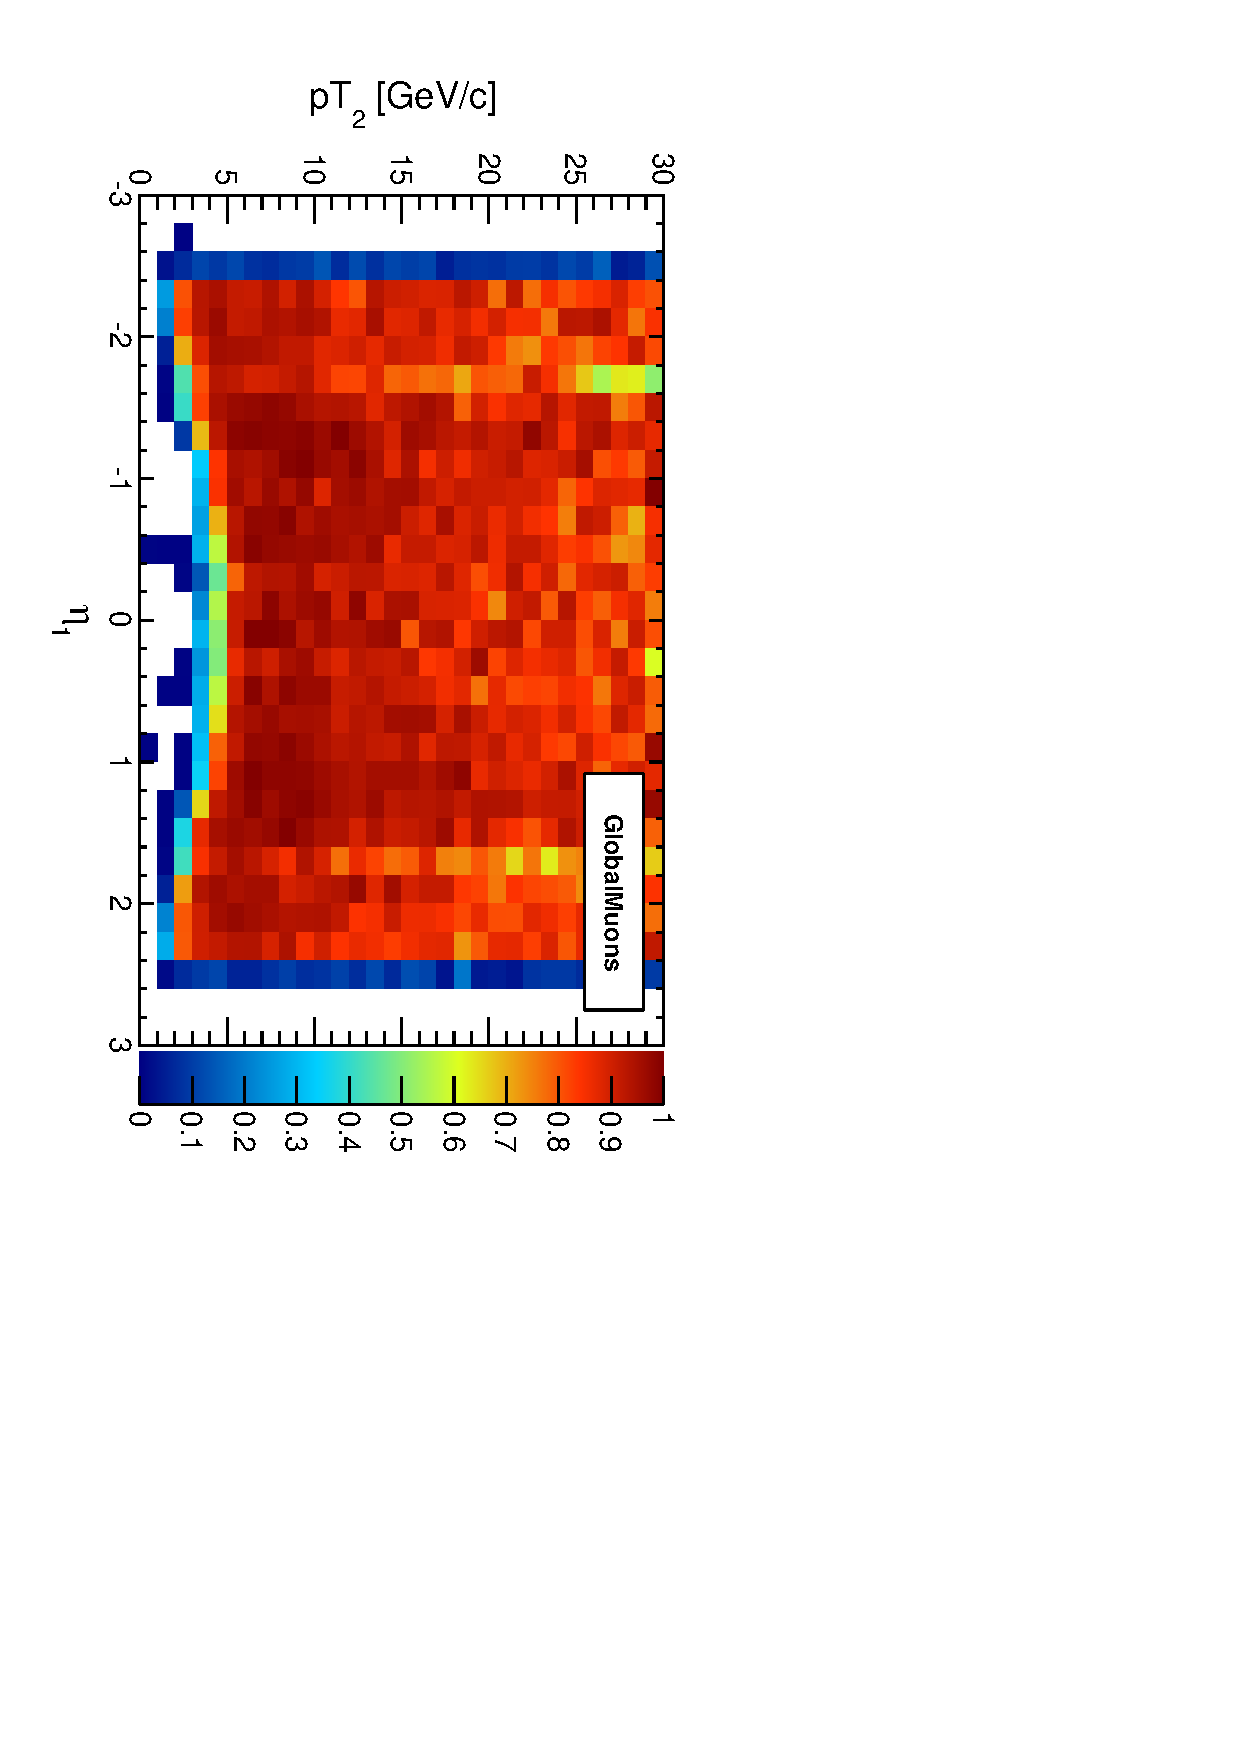
\includegraphics[height=0.45\linewidth, angle=90]{pt2vseta1_GlobalMuons.pdf}
\end{center}
\end{frame}

\begin{frame}
\frametitle{TrackerMuons vs.\ GlobalMuons}
\begin{itemize}\setlength{\itemsep}{0.25 cm}
\item TrackerMuons have high efficiency everywhere, but they also have (curably) high backgrounds
\item StandAloneMuon efficiency depends on how close the muons approach each other in the muon system (next slide)
\item GlobalMuon efficiency $\le$ StandAloneMuon efficiency
\begin{itemize}
\item probability of crossing in the muon system depends on kinematics of the decay
\item this would make it more complicated to quote limits on Lepton Jets derived from GlobalMuons
\end{itemize}
\item I tried StandAlone-SET because I knew that it is an alternative to the standard StandAloneMuons
\begin{itemize}
\item it doesn't seem to be designed for nearby-muon efficiency
\item we won't be using it
\end{itemize}
\end{itemize}
\end{frame}

\begin{frame}
\frametitle{Efficiency vs.\ crossing}
\begin{itemize}
\item StandAloneMuon inefficiencies are driven by reconstruction
  issues for muons that overlap in the muon system
\item Test: propagate generator-level muons to planes of constant-$z$
  in the endcap and cylinders around the beamline in the barrel
\item Plot efficiency as a function of trajectory intersections:
  $\Delta \phi_\s{ME2}$ is $\phi_{\mu^+} - \phi_{\mu^-}$ at $z =
  828.561$~cm, $\Delta R\s{ME2}$ is radial difference
\end{itemize}
\begin{center}
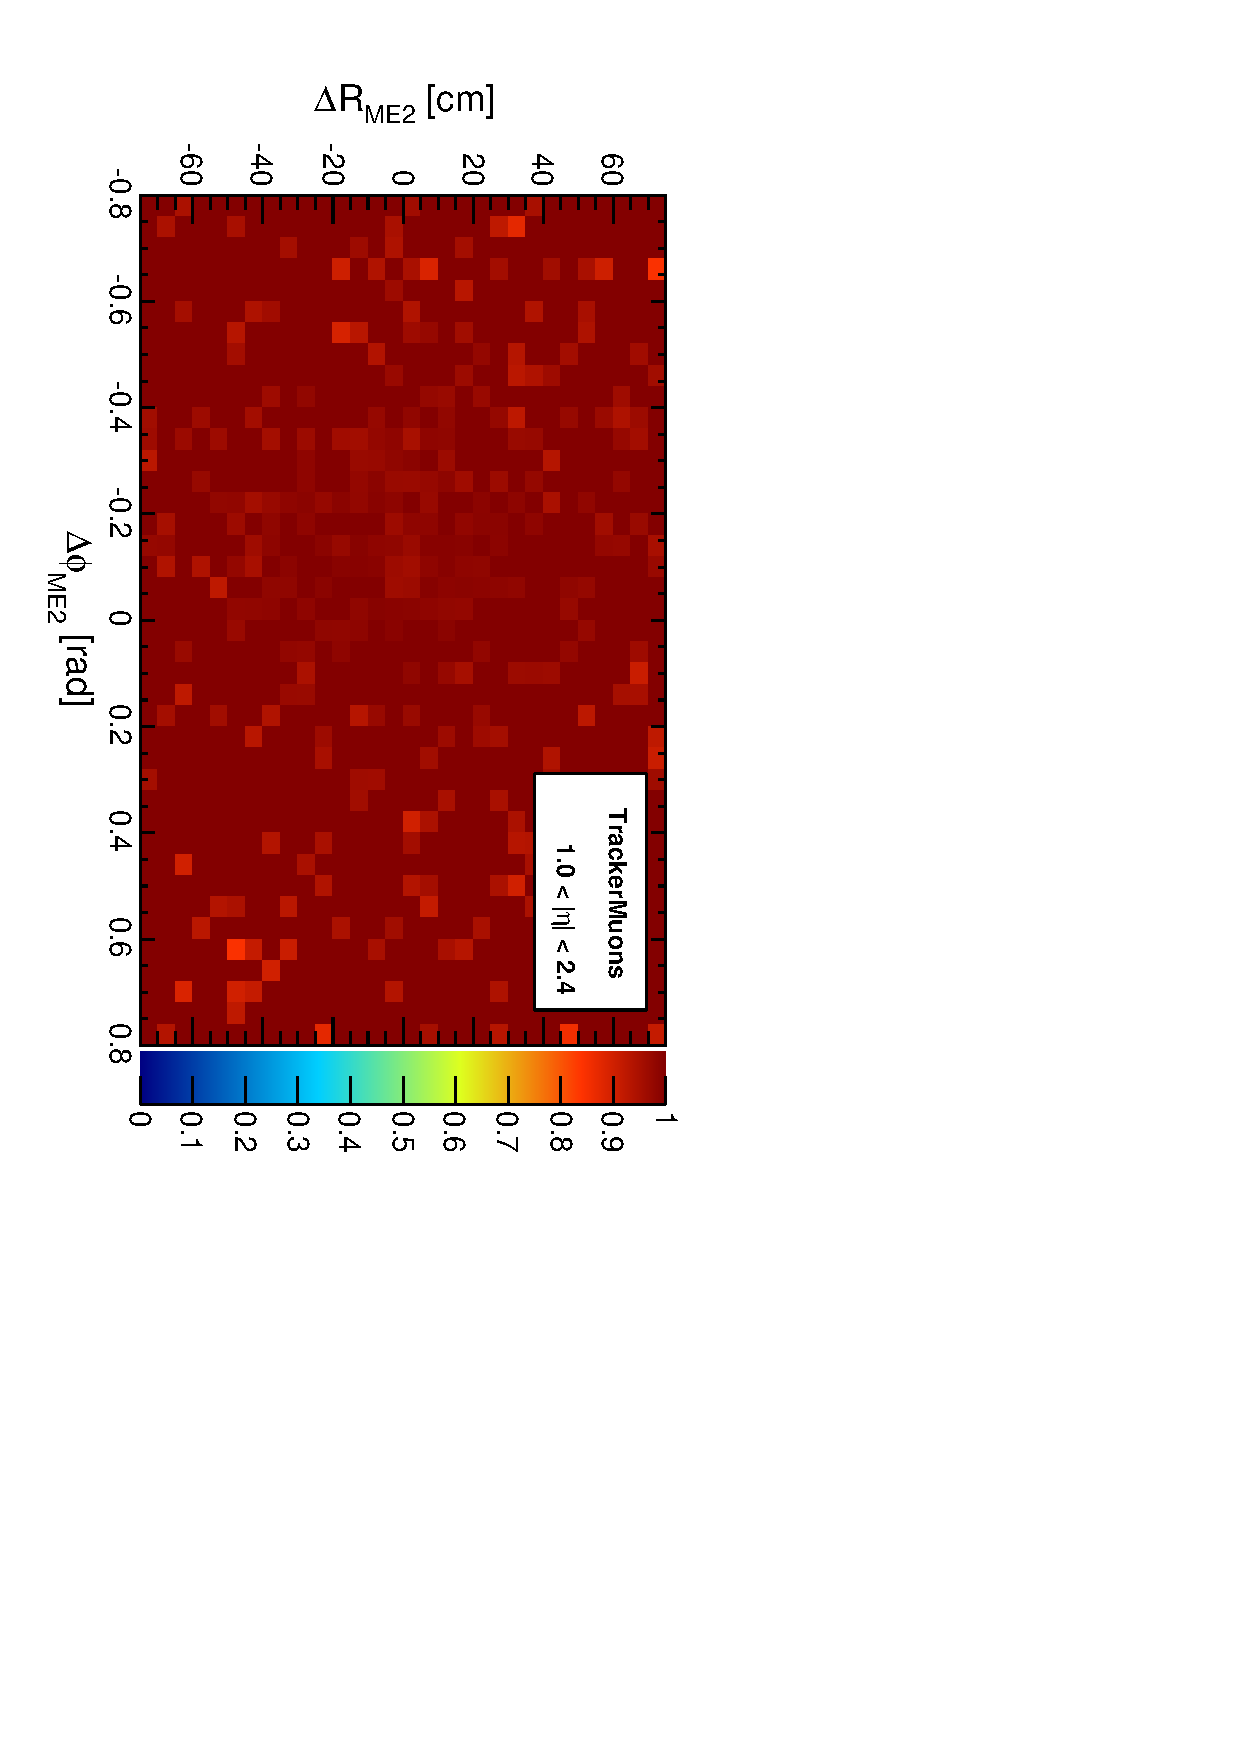
\includegraphics[height=0.45\linewidth, angle=90]{me2_TrackerMuons.pdf}
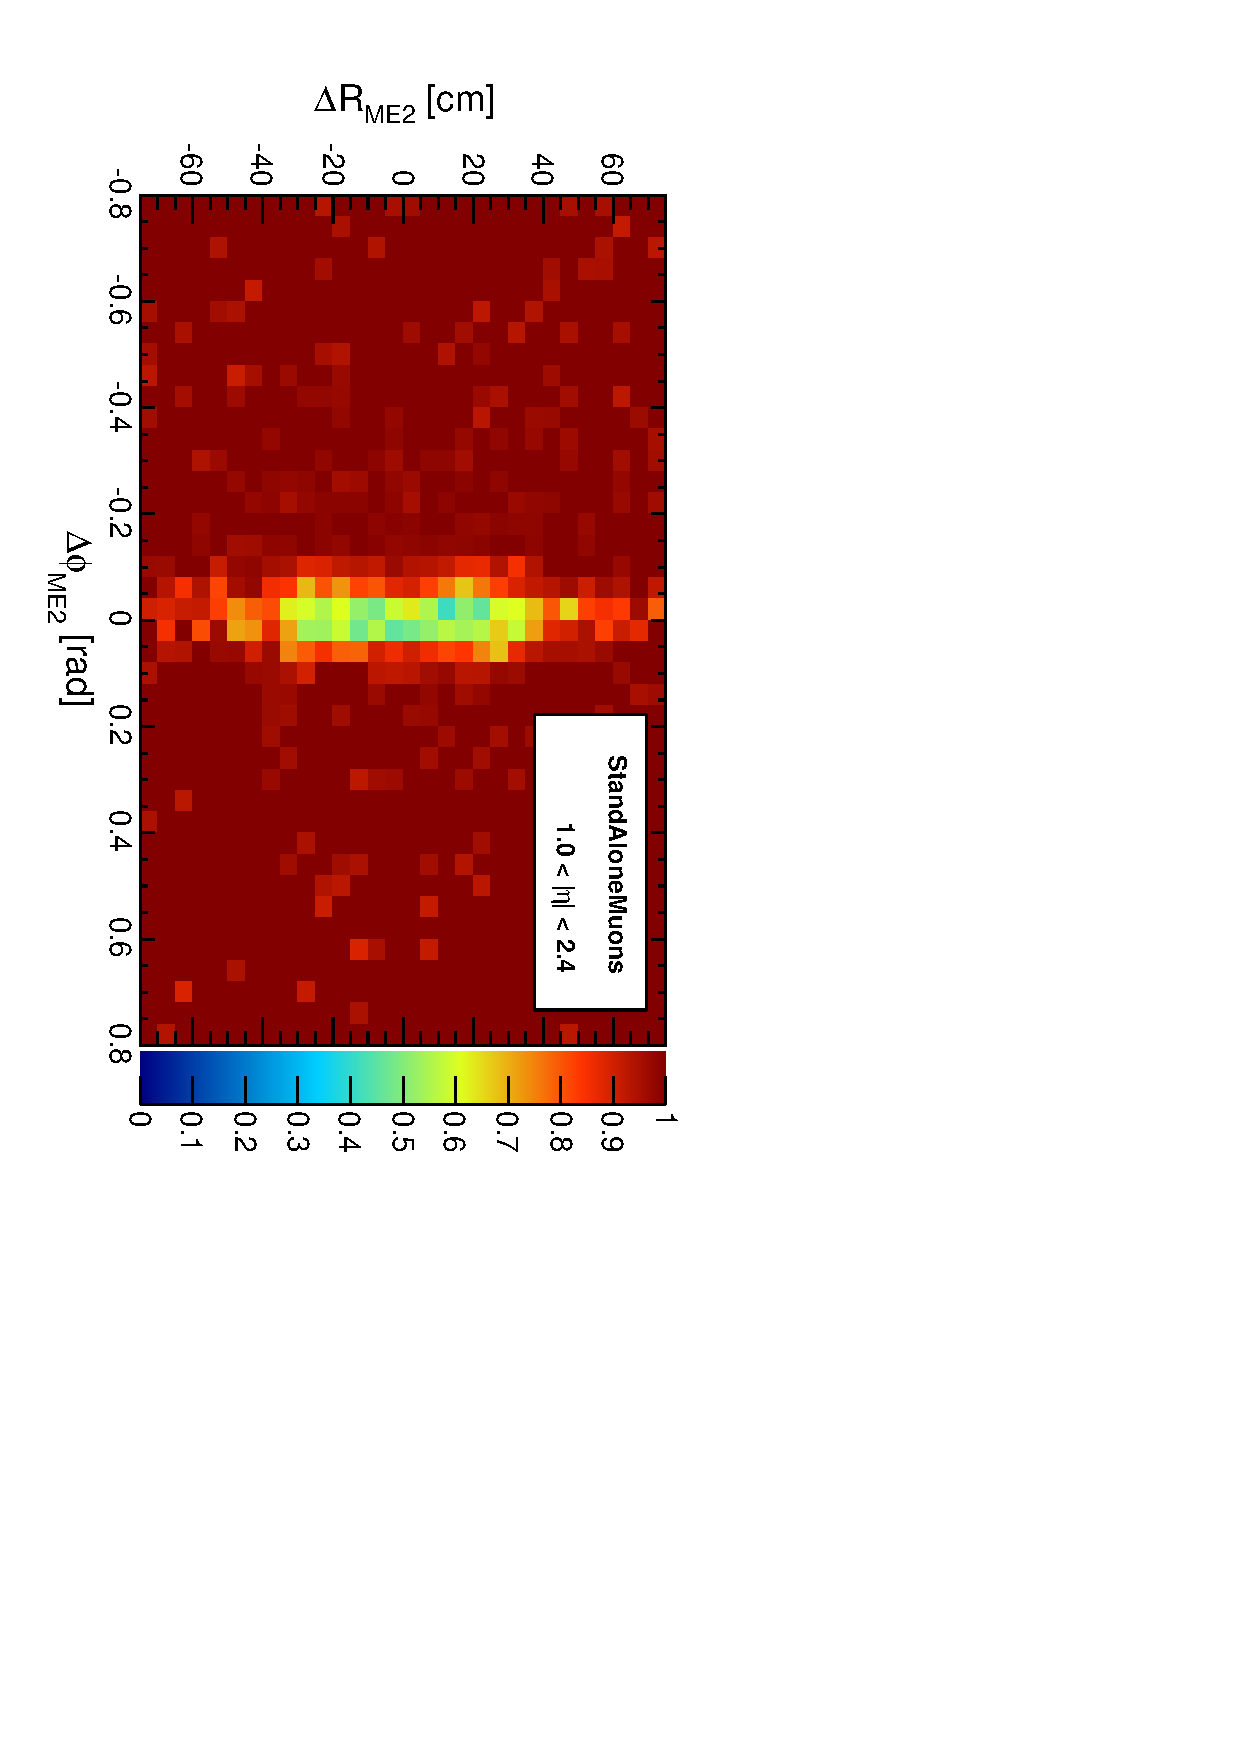
\includegraphics[height=0.45\linewidth, angle=90]{me2_StandAloneUpdatedDefault.pdf}

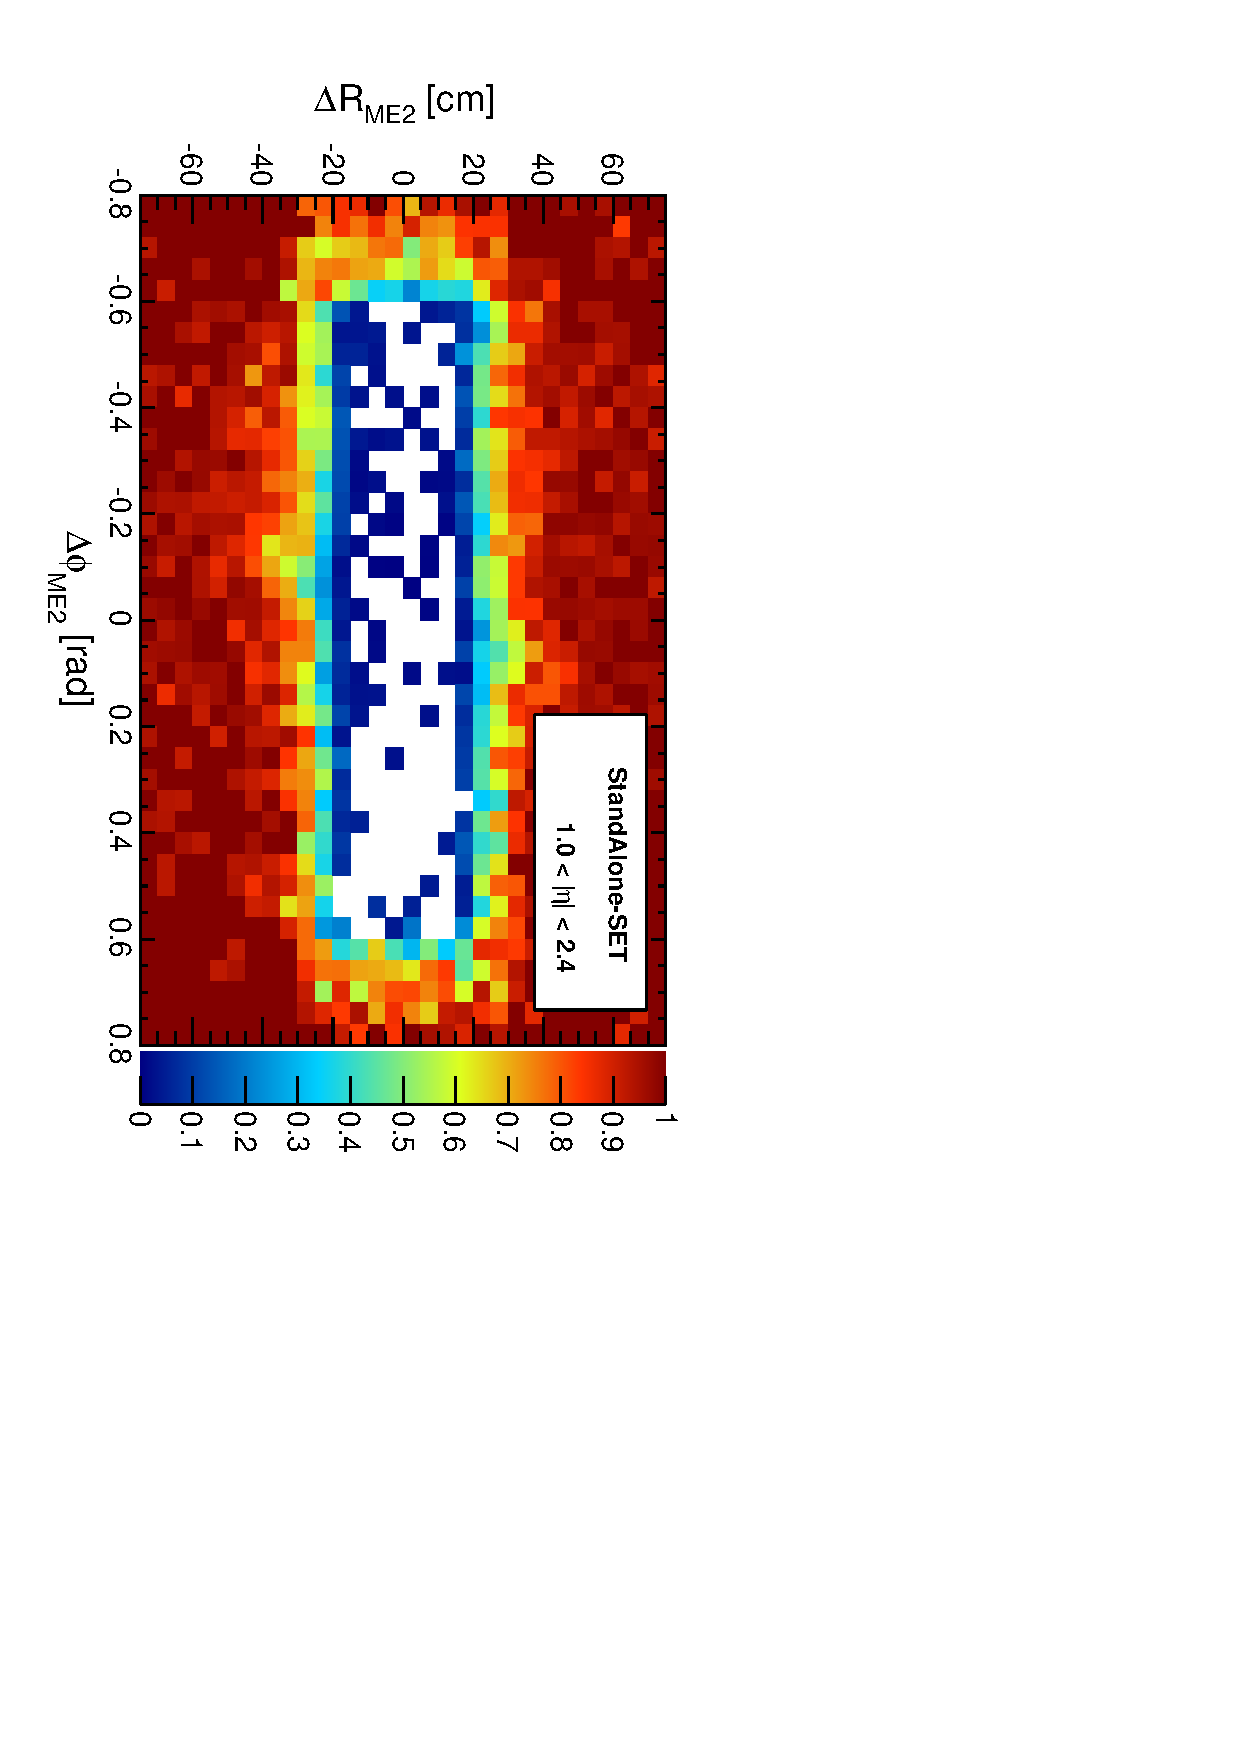
\includegraphics[height=0.45\linewidth, angle=90]{me2_StandAloneUpdatedSET.pdf}
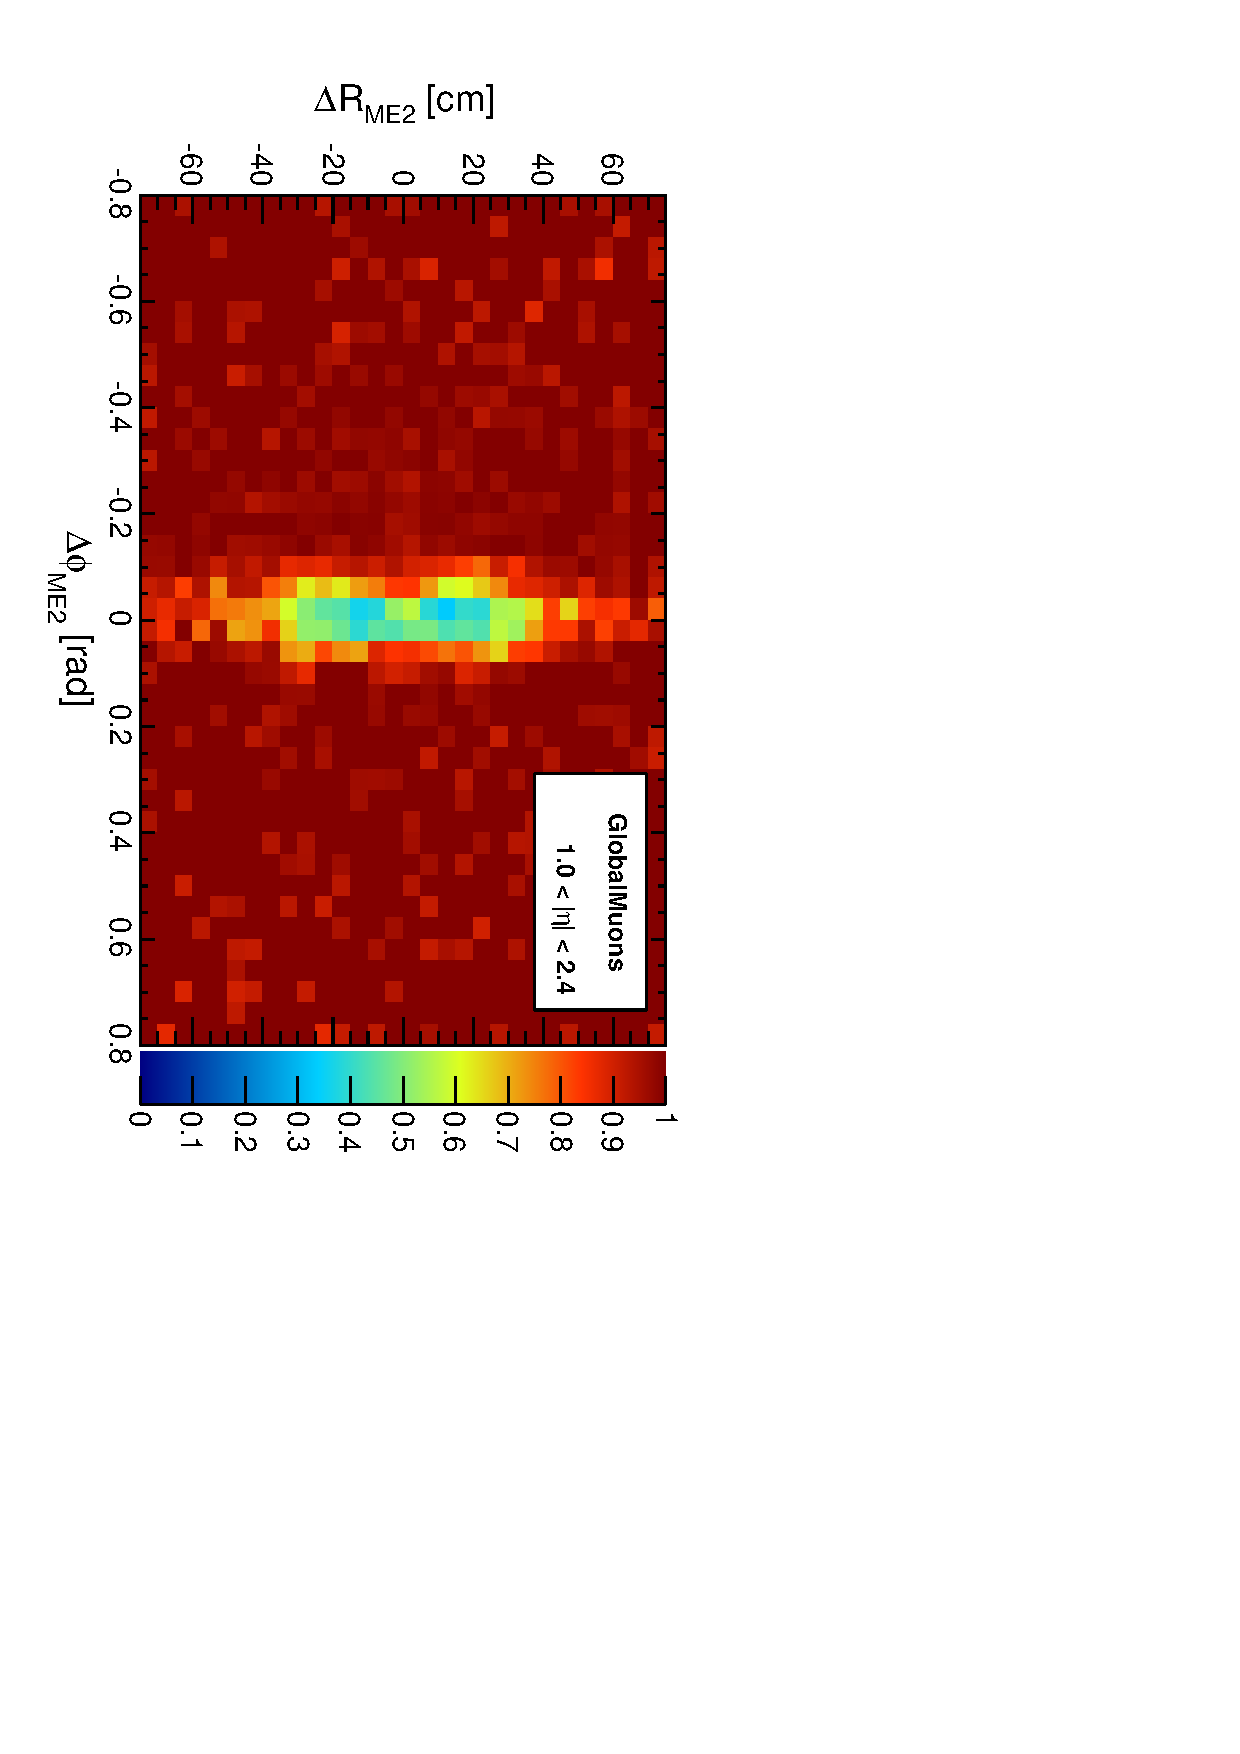
\includegraphics[height=0.45\linewidth, angle=90]{me2_GlobalMuons.pdf}
\end{center}
\end{frame}

\begin{frame}
\frametitle{Efficiency vs.\ crossing}
\begin{itemize}
\item Same thing in the barrel: $\Delta \phi_{MB3}$ and $\Delta
  Z_{MB3}$ on a cylinder of radius 618.269~cm
\item Not completely understood: inefficiencies are off-centered from
  zero
\item Suggests that this plot is ``out of focus''--- the intersection
  that drives inefficiency is perhaps at smaller radius than barrel?
\end{itemize}

\begin{center}
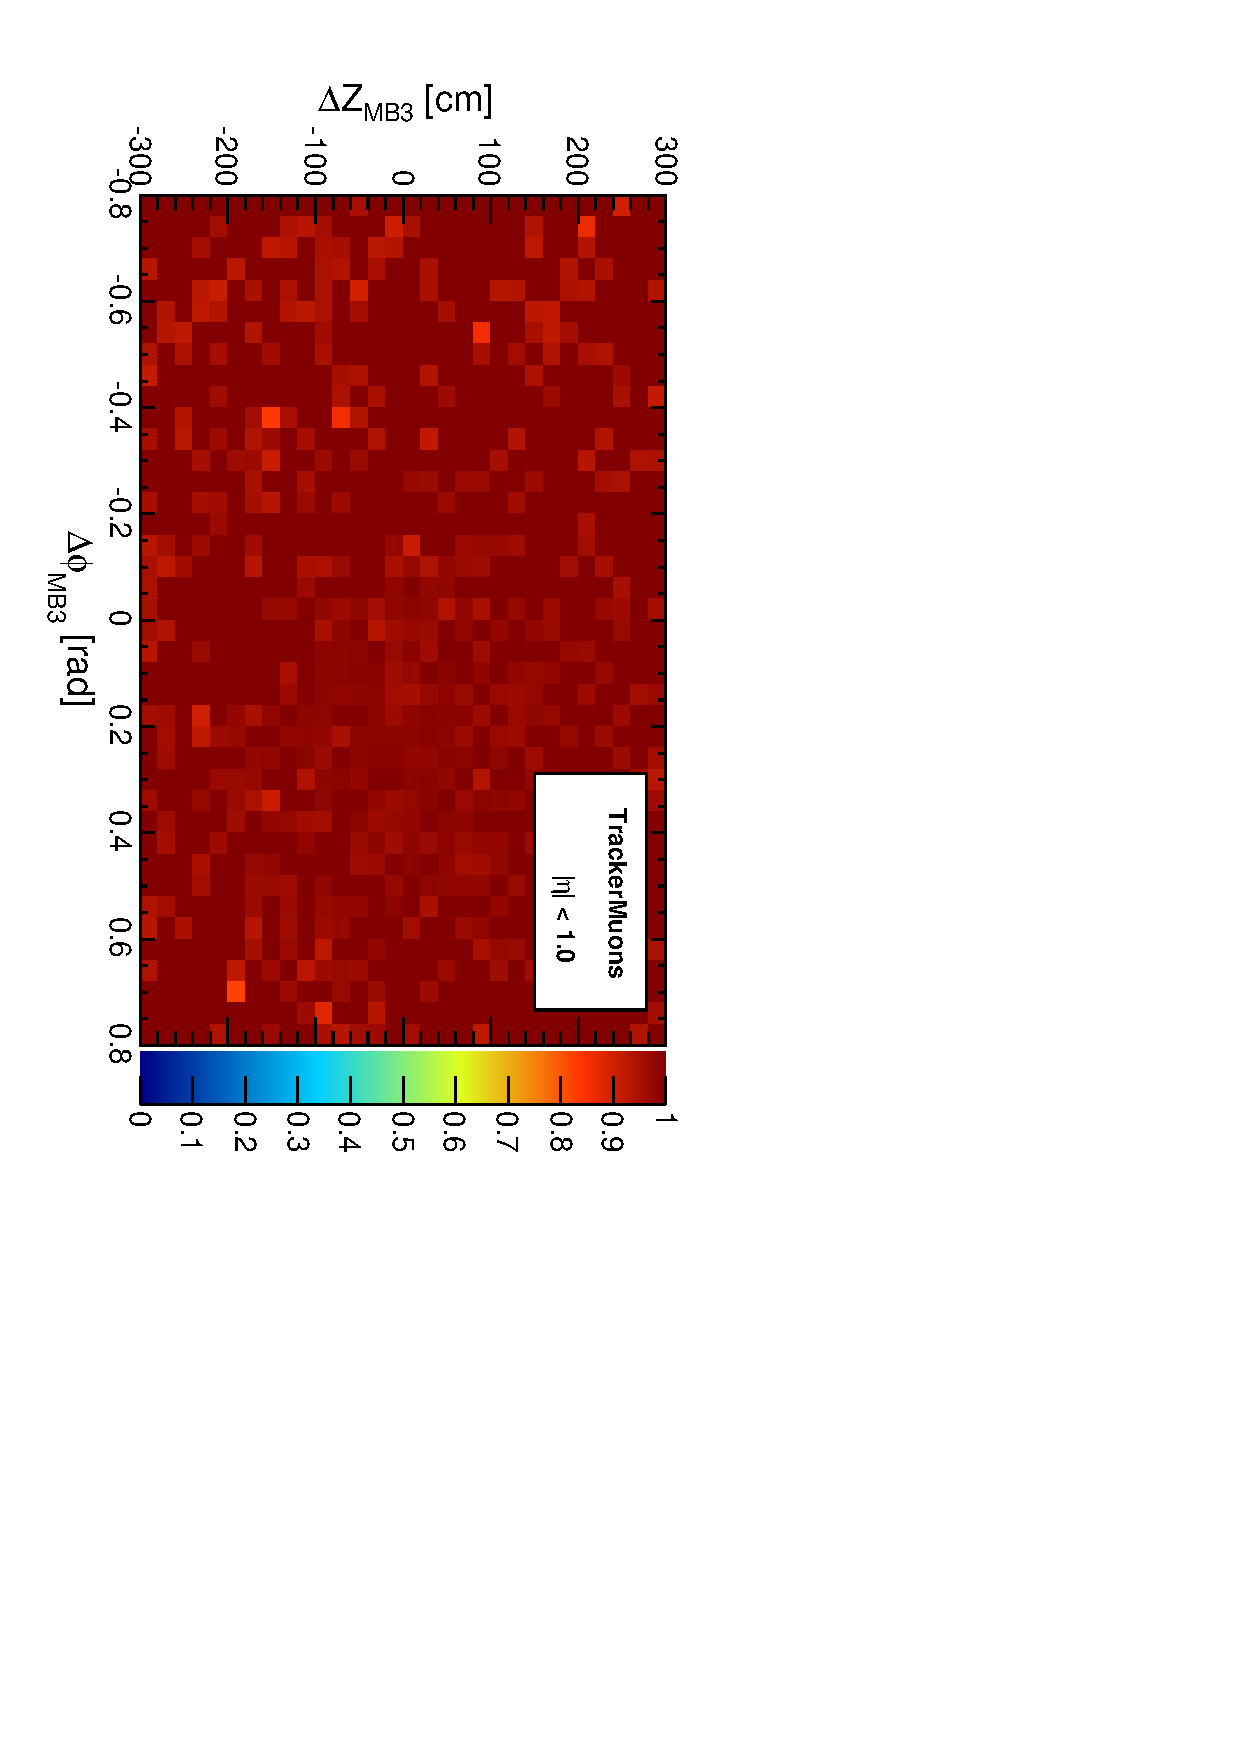
\includegraphics[height=0.45\linewidth, angle=90]{mb3_TrackerMuons.pdf}
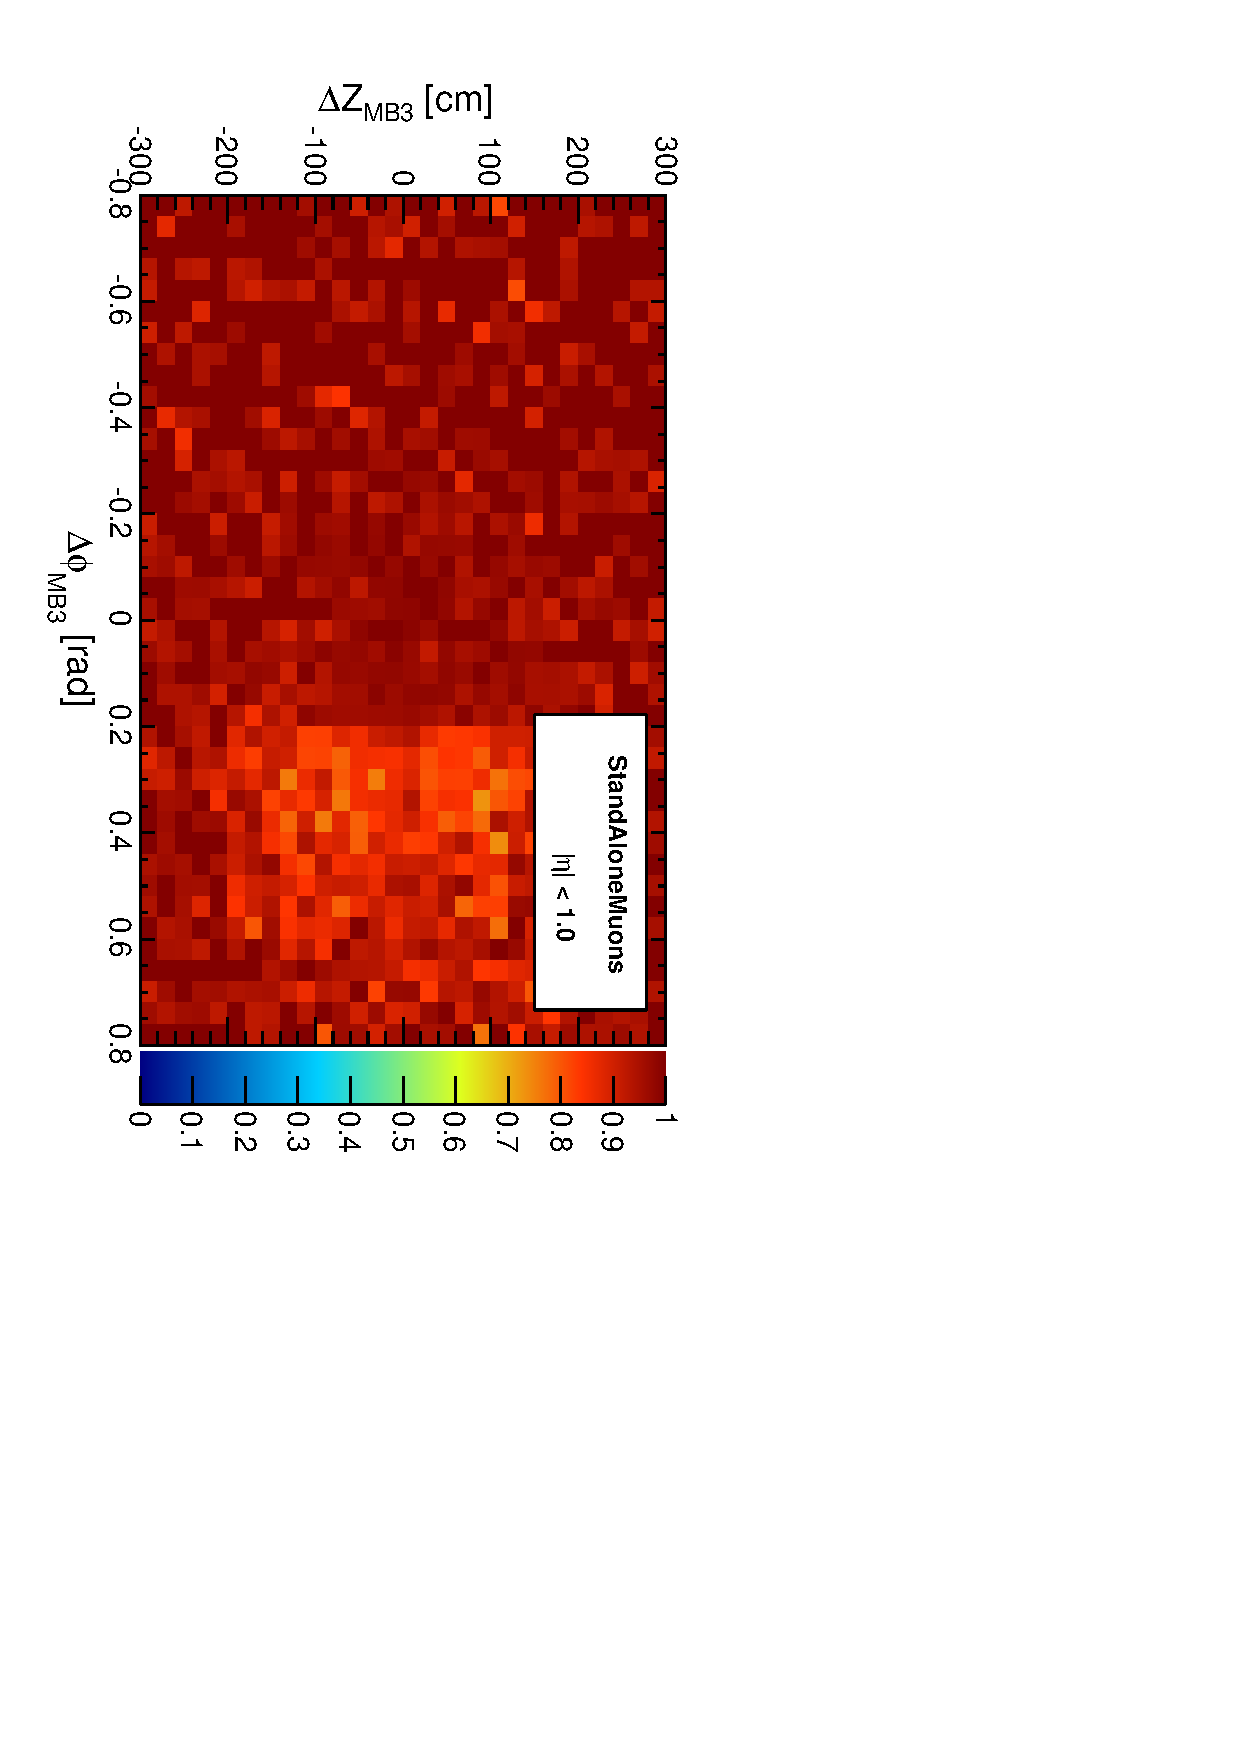
\includegraphics[height=0.45\linewidth, angle=90]{mb3_StandAloneUpdatedDefault.pdf}

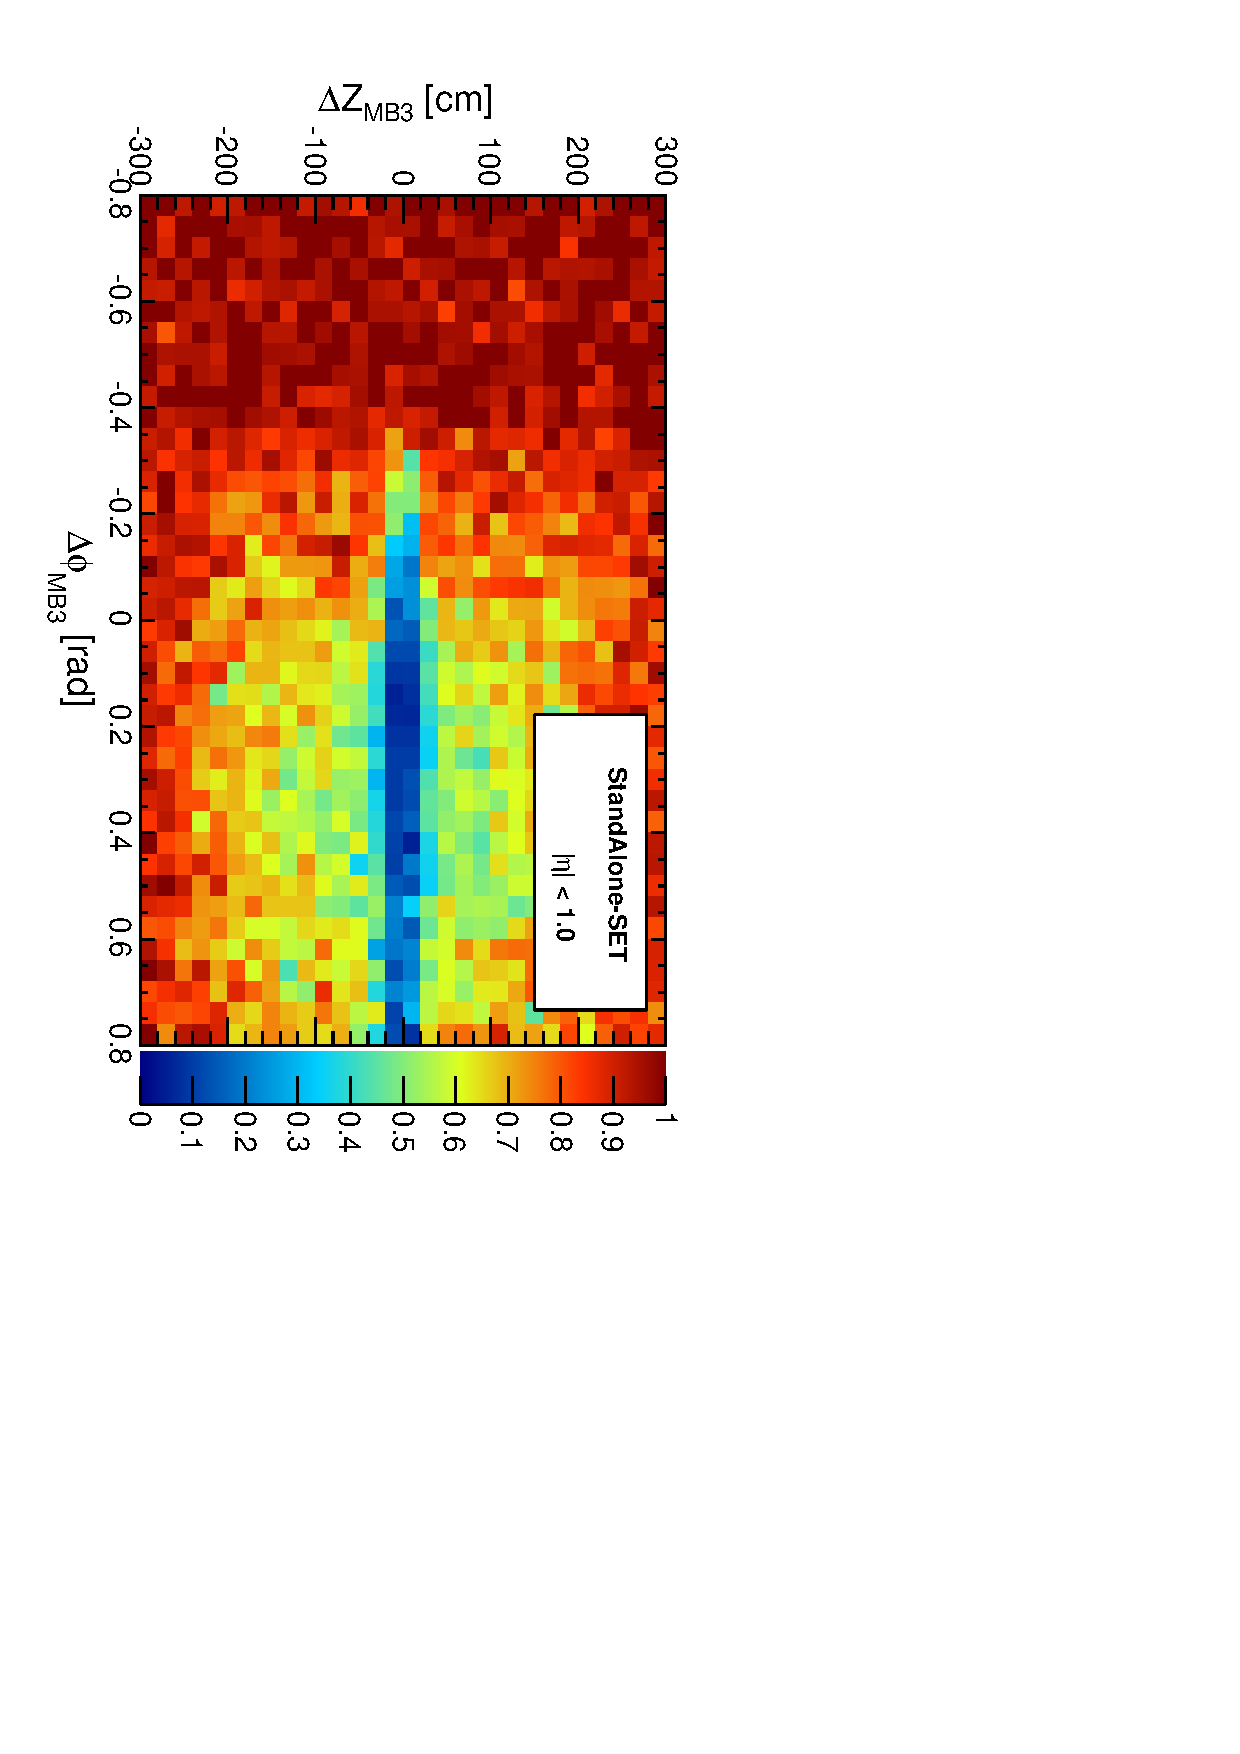
\includegraphics[height=0.45\linewidth, angle=90]{mb3_StandAloneUpdatedSET.pdf}
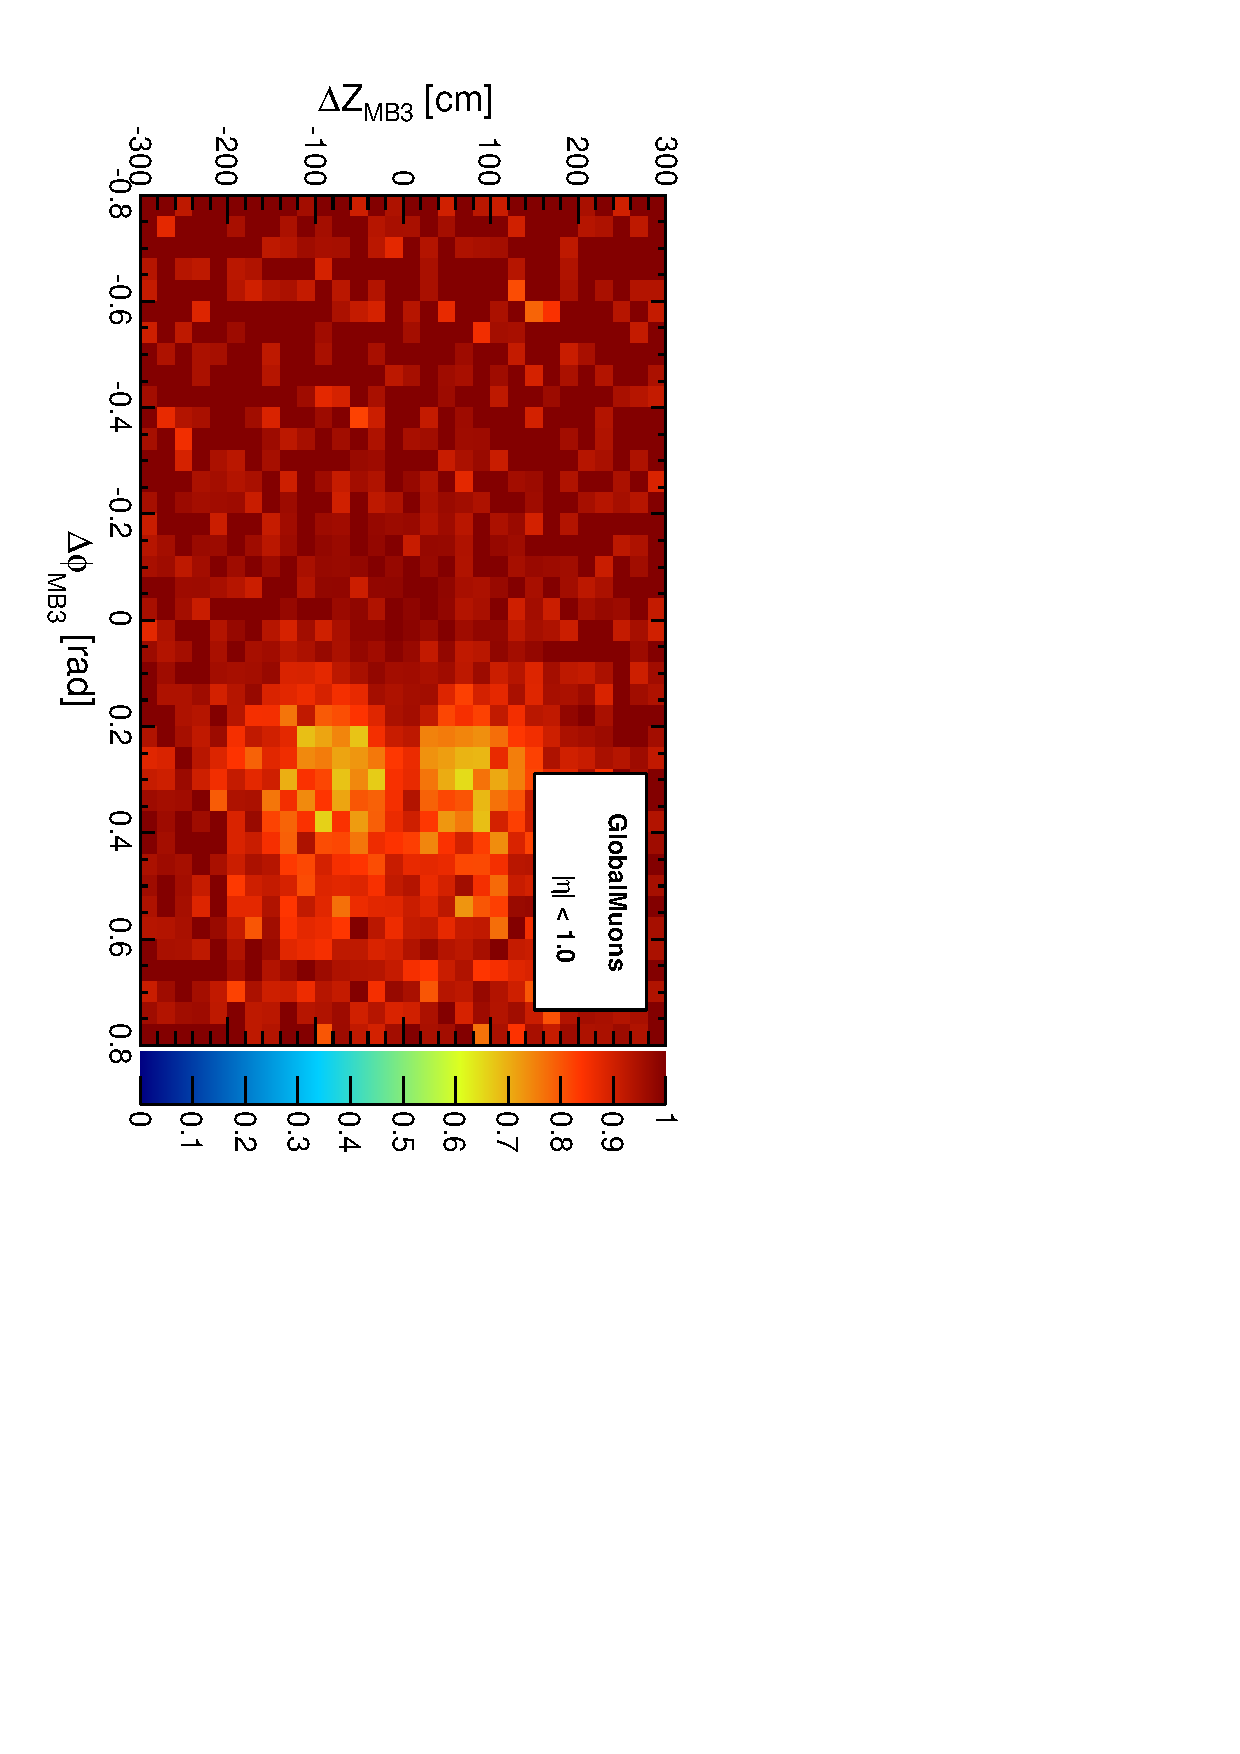
\includegraphics[height=0.45\linewidth, angle=90]{mb3_GlobalMuons.pdf}
\end{center}
\end{frame}

\begin{frame}
\frametitle{TrackerMuon Backgrounds}
\begin{itemize}
\item Before moving on, we should address \mbox{backgrounds with TrackerMuons\hspace{-1 cm}}
\item Number of reconstructed muons $N_\s{muons}$ in the InclusiveMu5\_Pt* samples (all QCD backgrounds, including decay-in-flight):

\begin{center}
\begin{columns}
\column{0.75\linewidth}
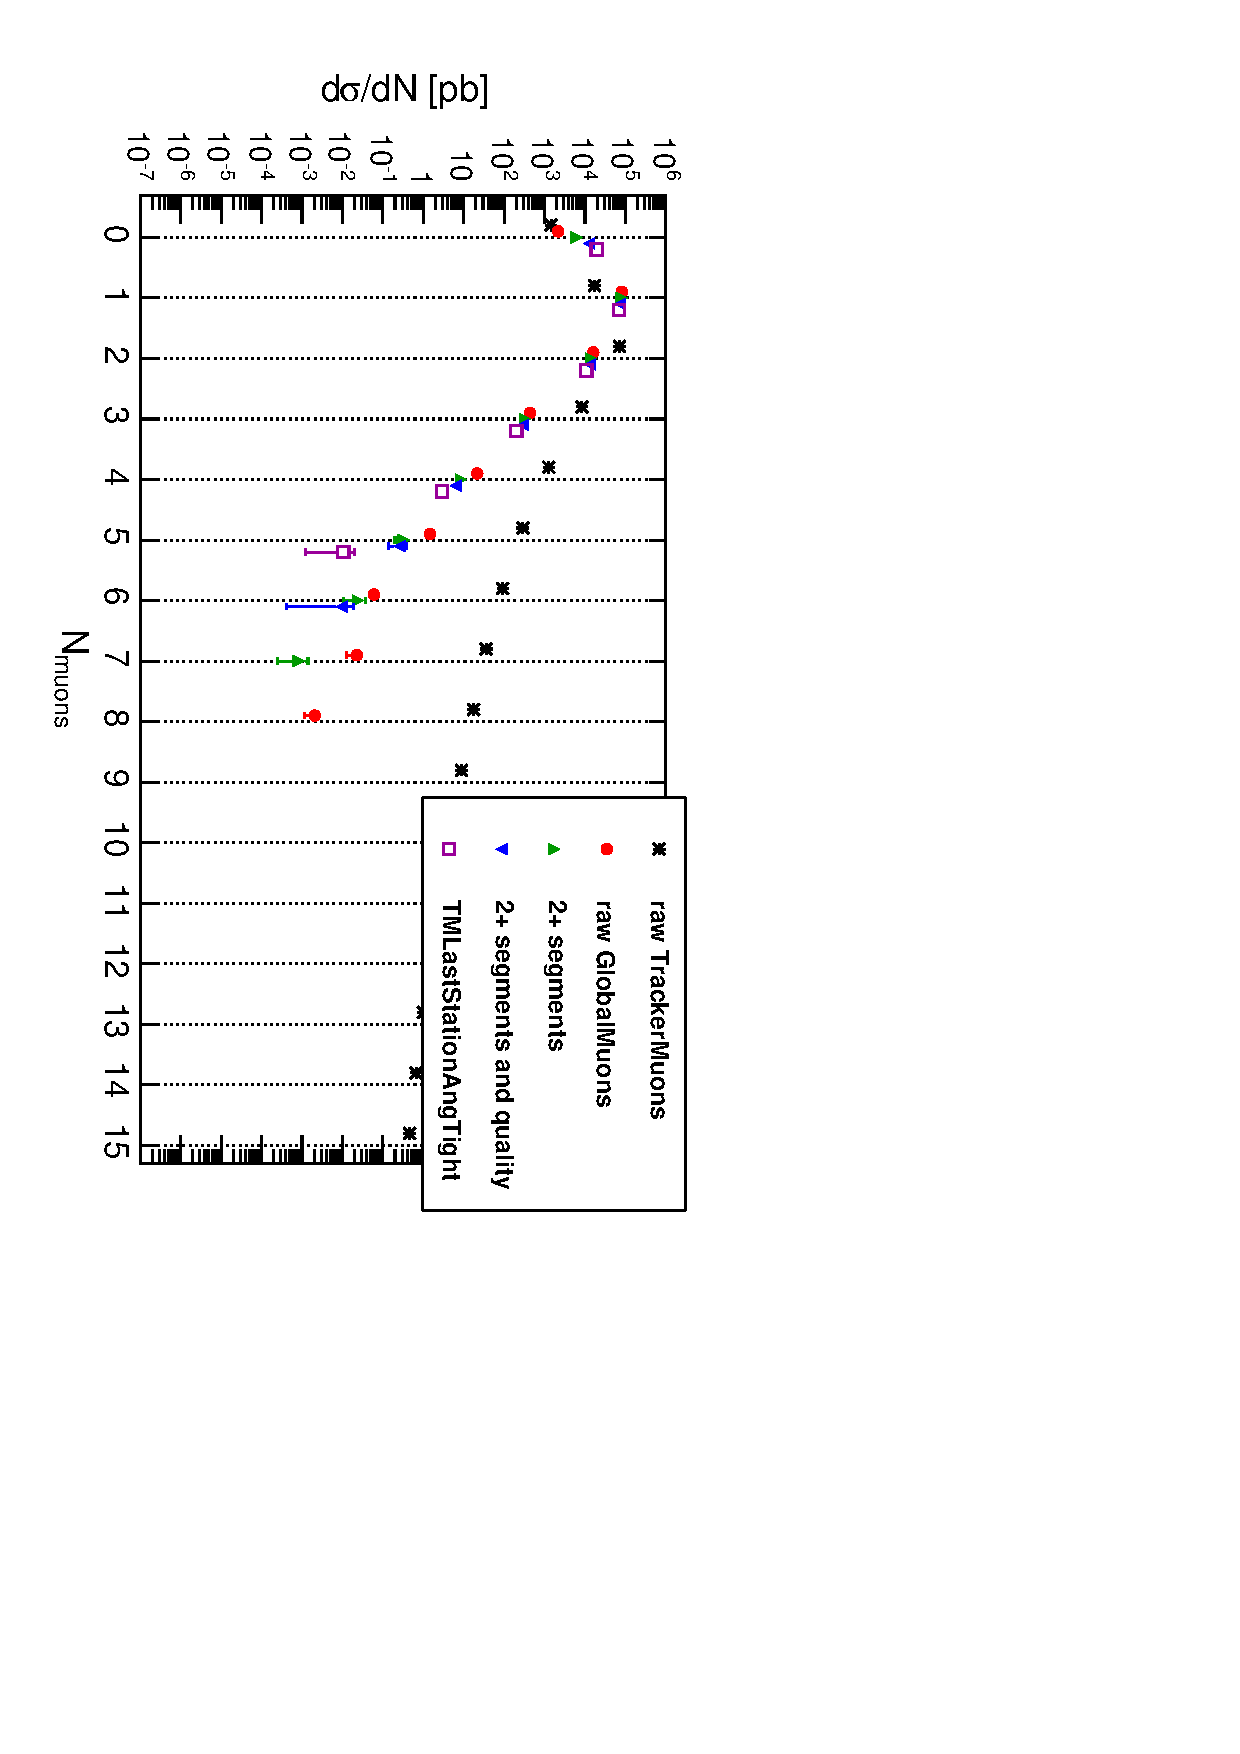
\includegraphics[height=\linewidth, angle=90]{tracks_samepage_allreal.pdf}

\column{0.25\linewidth}
\scriptsize All sets of track cuts include $p_T > 5$~GeV/$c$

\vspace{0.25 cm}
``Quality'' means

\vspace{0.1 cm}
$N_\s{trkr hits} \ge 8$

\vspace{0.1 cm}
${\chi^2}_\s{trkr}/N_\s{dof} < 5$

\vspace{0.1 cm}
$\sigma_\phi < 0.03$

\vspace{0.1 cm}
$\sigma_\eta < 0.01$

\vspace{0.1 cm}
$\sigma_{d_{xy}} < 0.05$~cm

\vspace{0.1 cm}
$\sigma_{d_z} < 0.1$~cm
\end{columns}
\end{center}

\item The {\it one cut} that makes TrackerMuons as pure as other
  reconstruction methods is $N_\s{segments} \ge 2$ for arbitrated
  segments
\end{itemize}
\end{frame}

\begin{frame}
\frametitle{TrackerMuon Backgrounds}
\begin{itemize}
\item Same plot, split up by the number of real muons in the event
\item As you can see, TrackerMuons with $N_\s{segments} \ge 2$ (green
  triangles) are narrowly distributed around the true number of muons
\end{itemize}

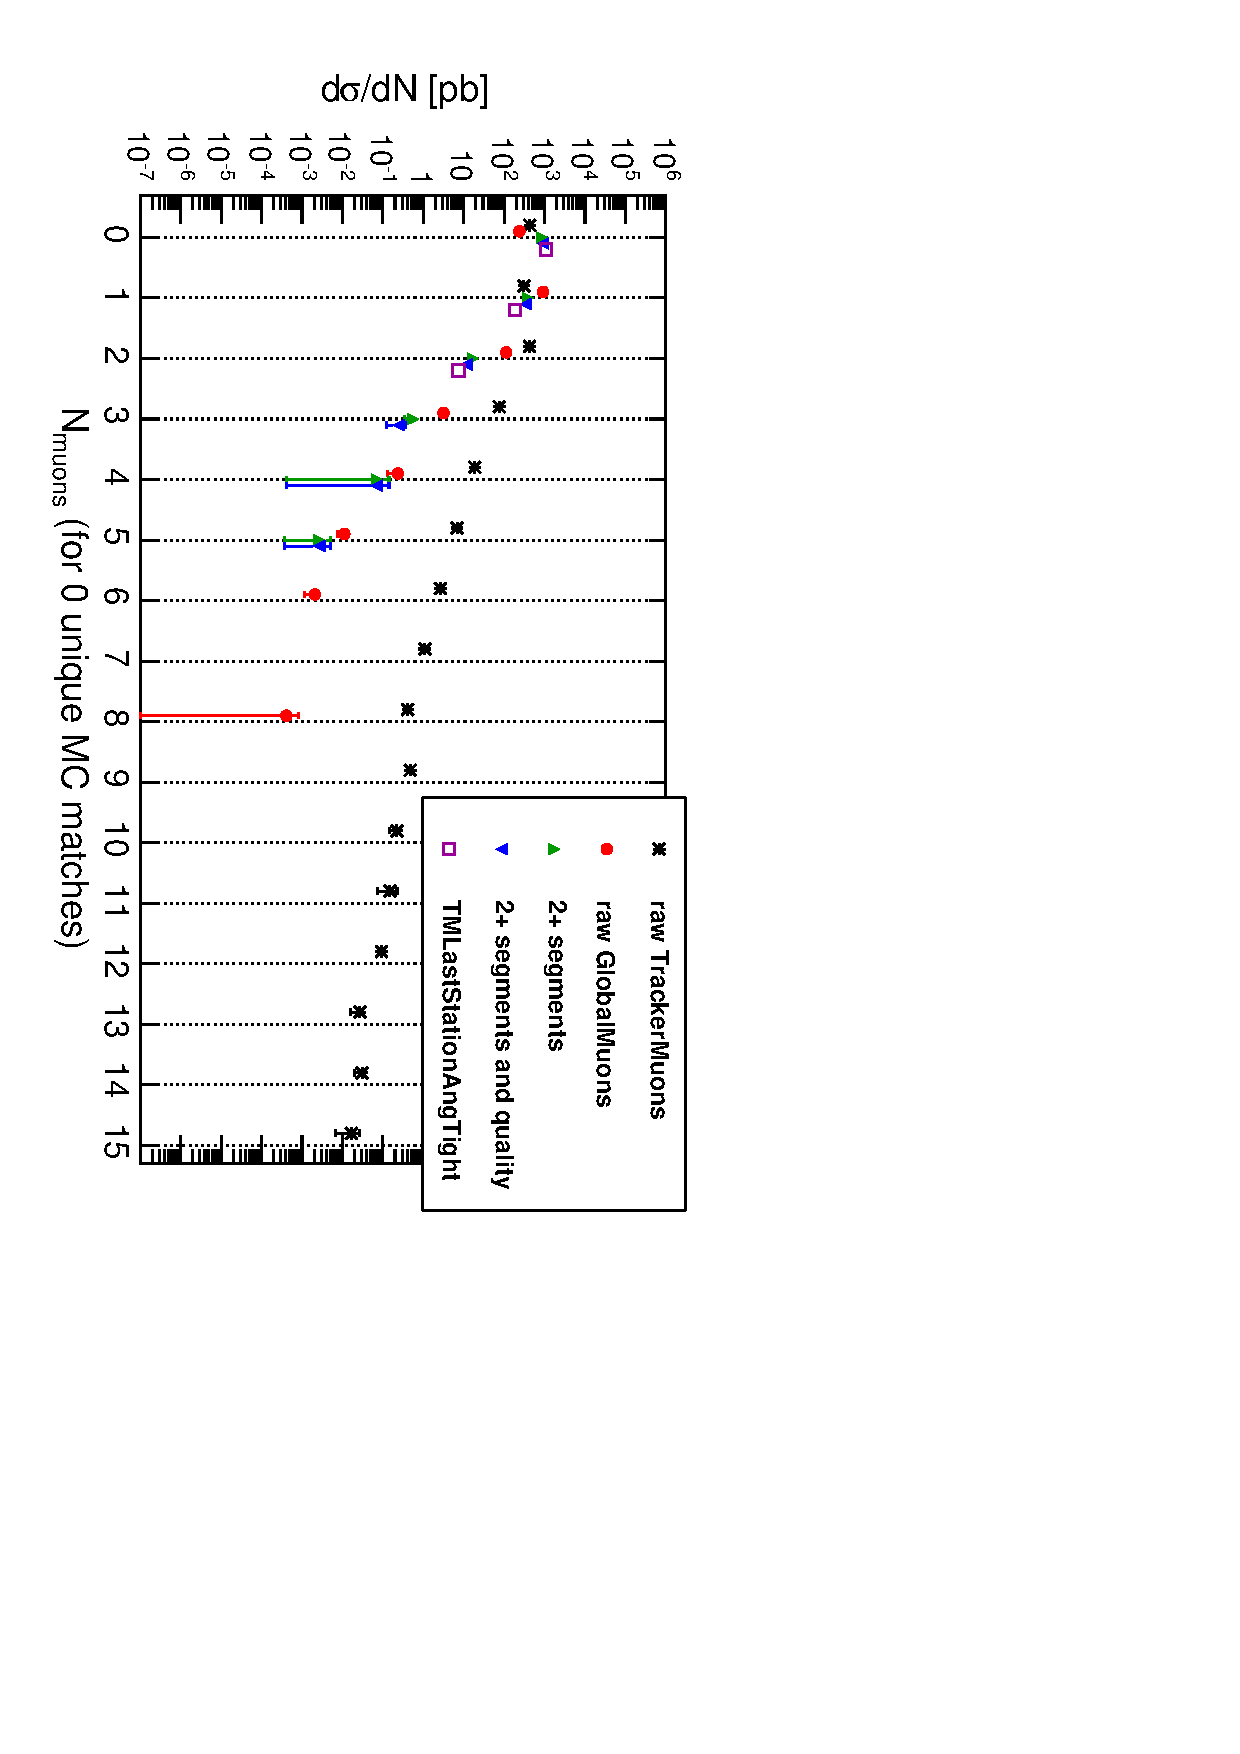
\includegraphics[height=0.5\linewidth, angle=90]{tracks_samepage_0real.pdf}
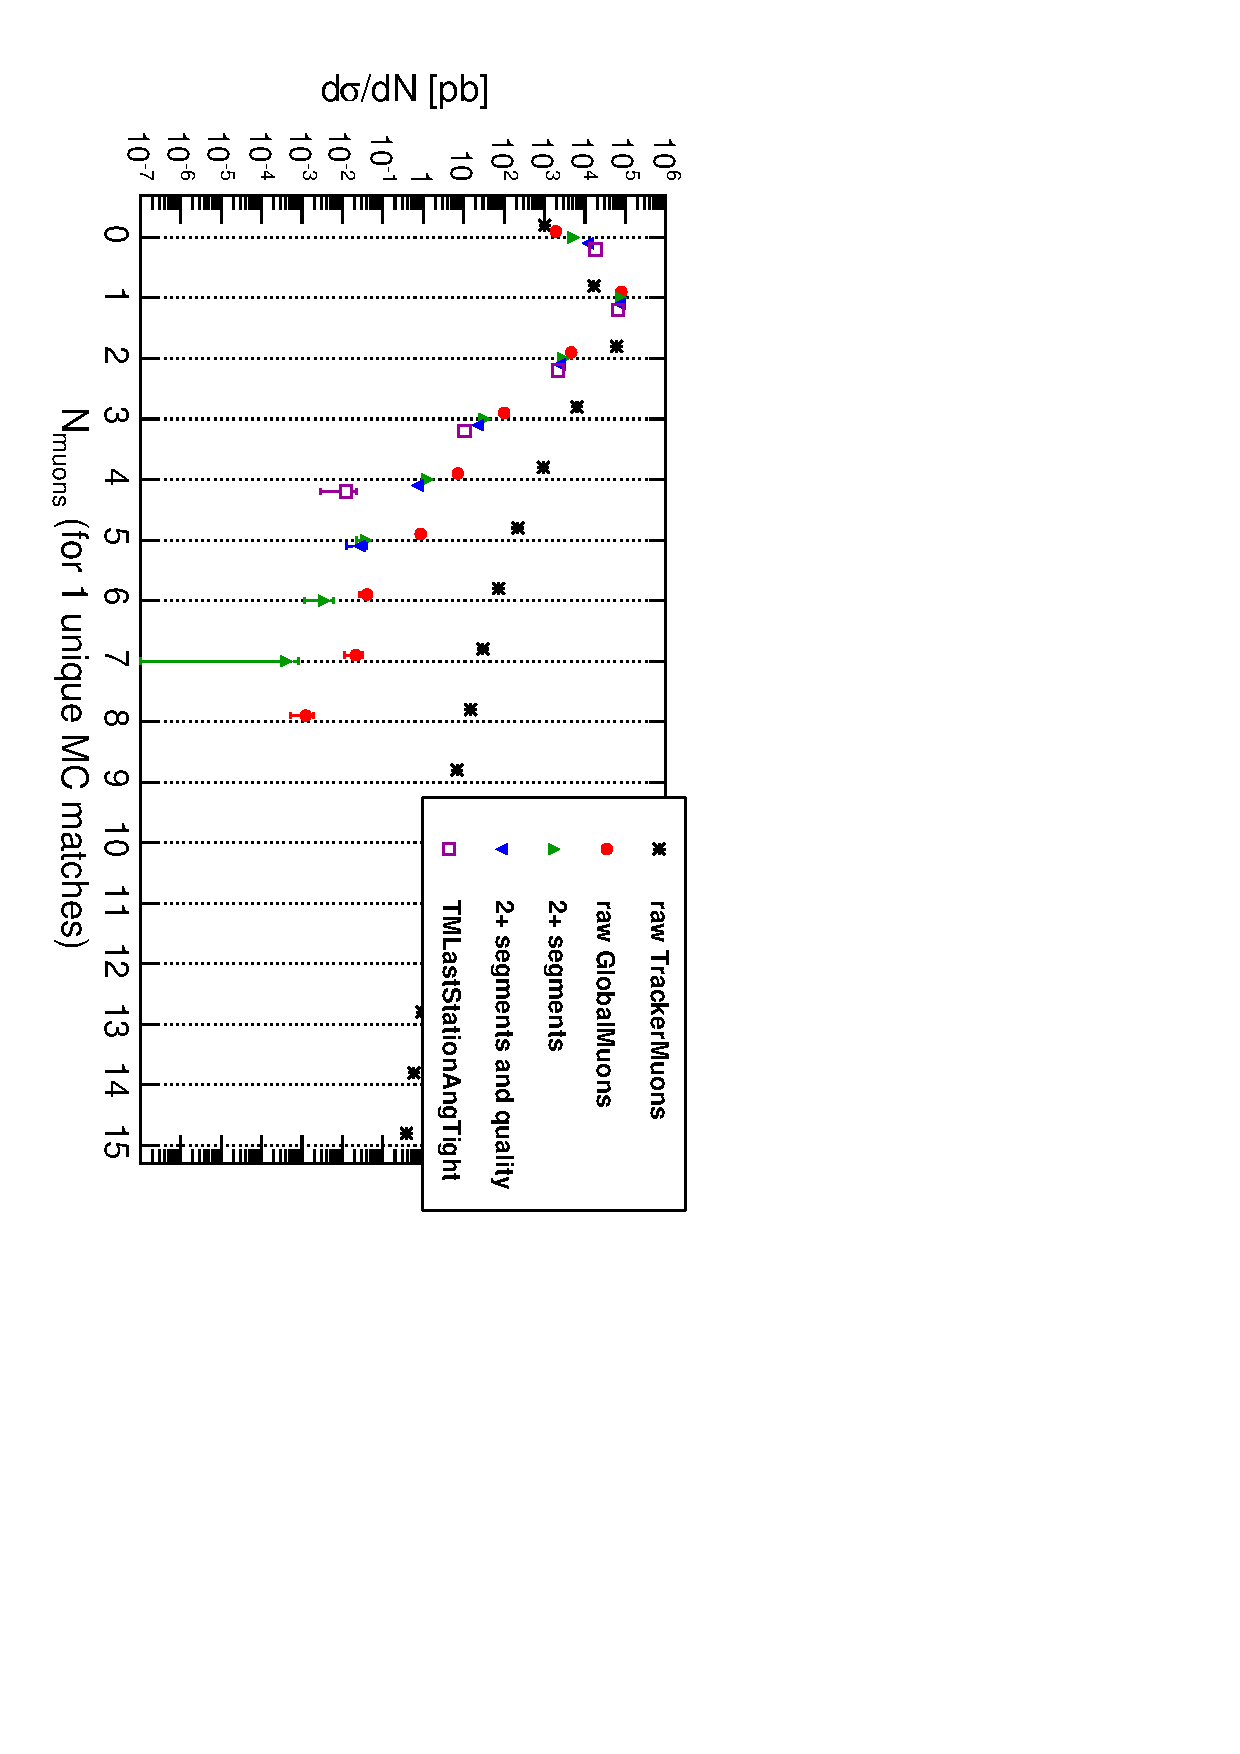
\includegraphics[height=0.5\linewidth, angle=90]{tracks_samepage_1real.pdf}

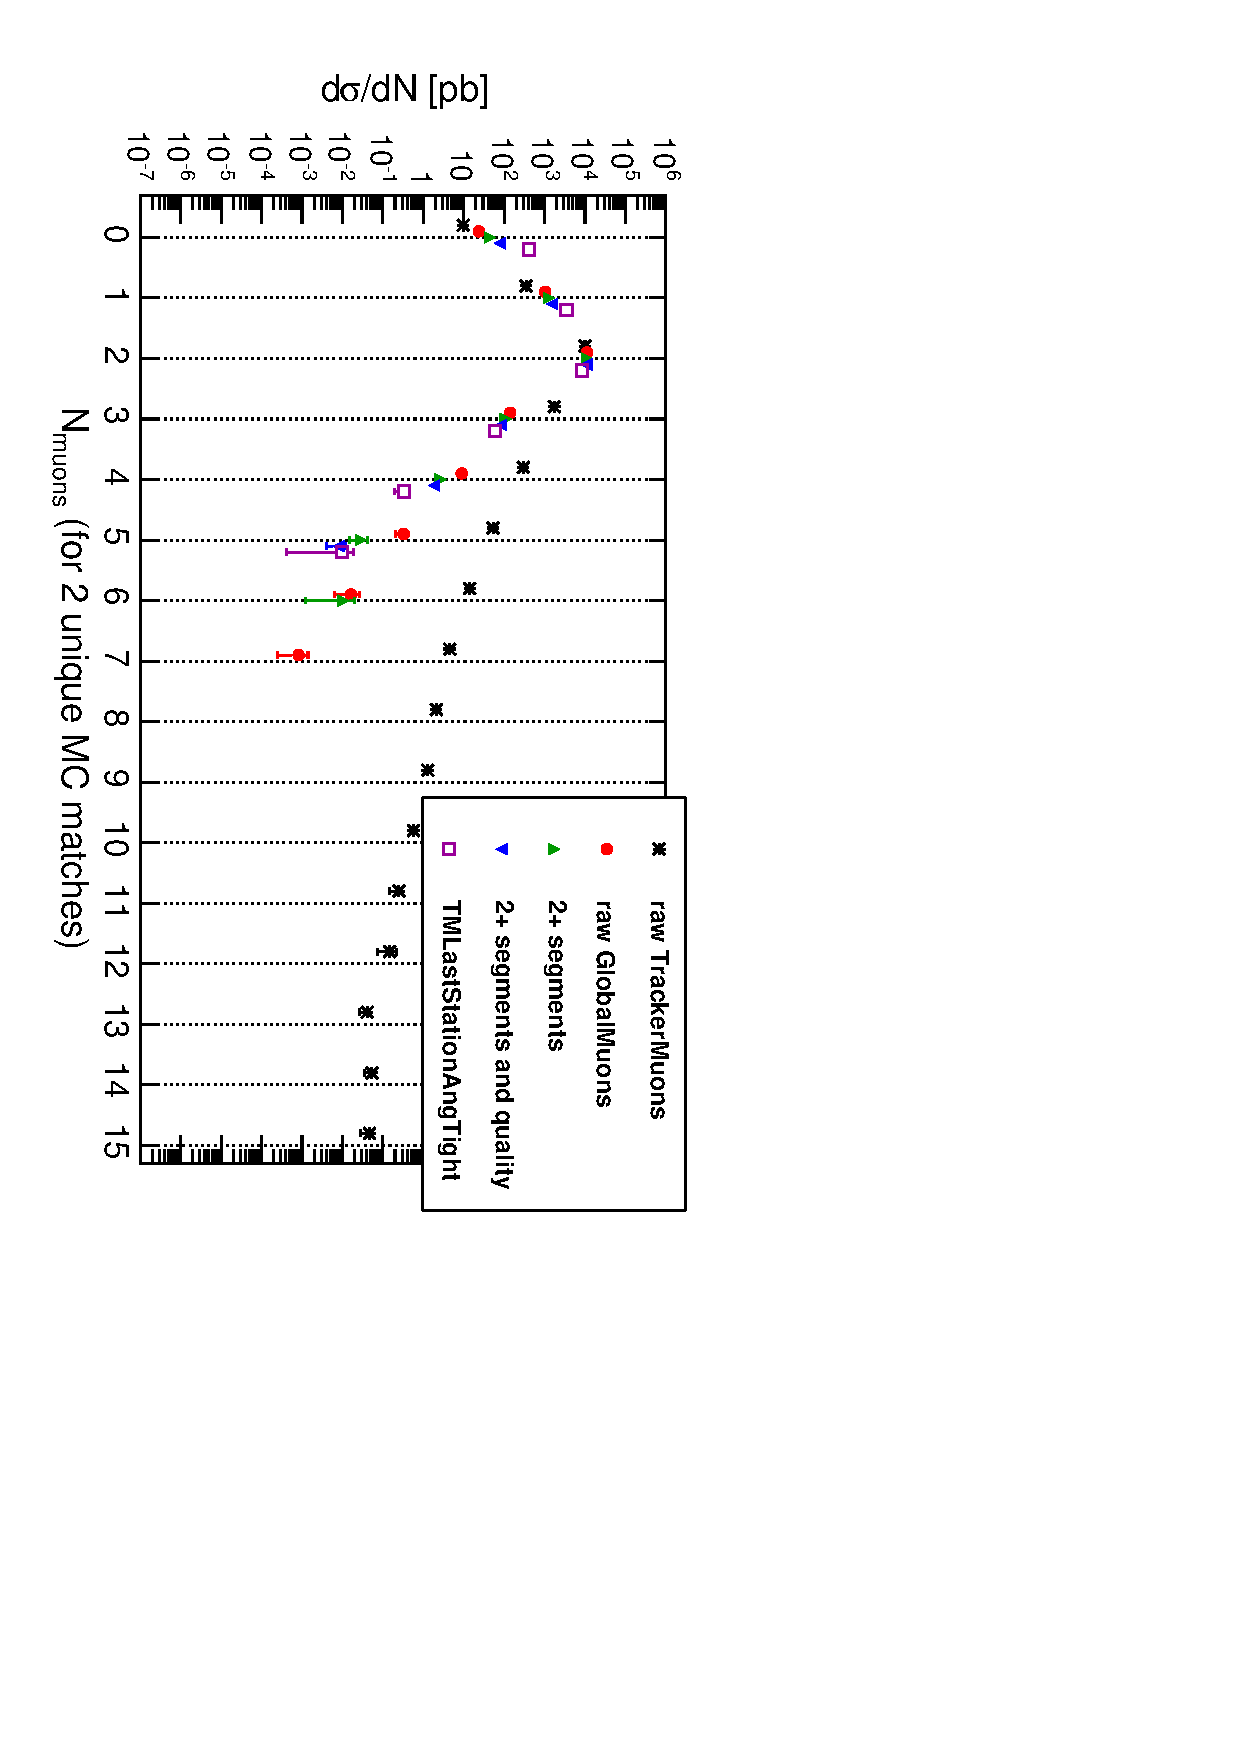
\includegraphics[height=0.5\linewidth, angle=90]{tracks_samepage_2real.pdf}
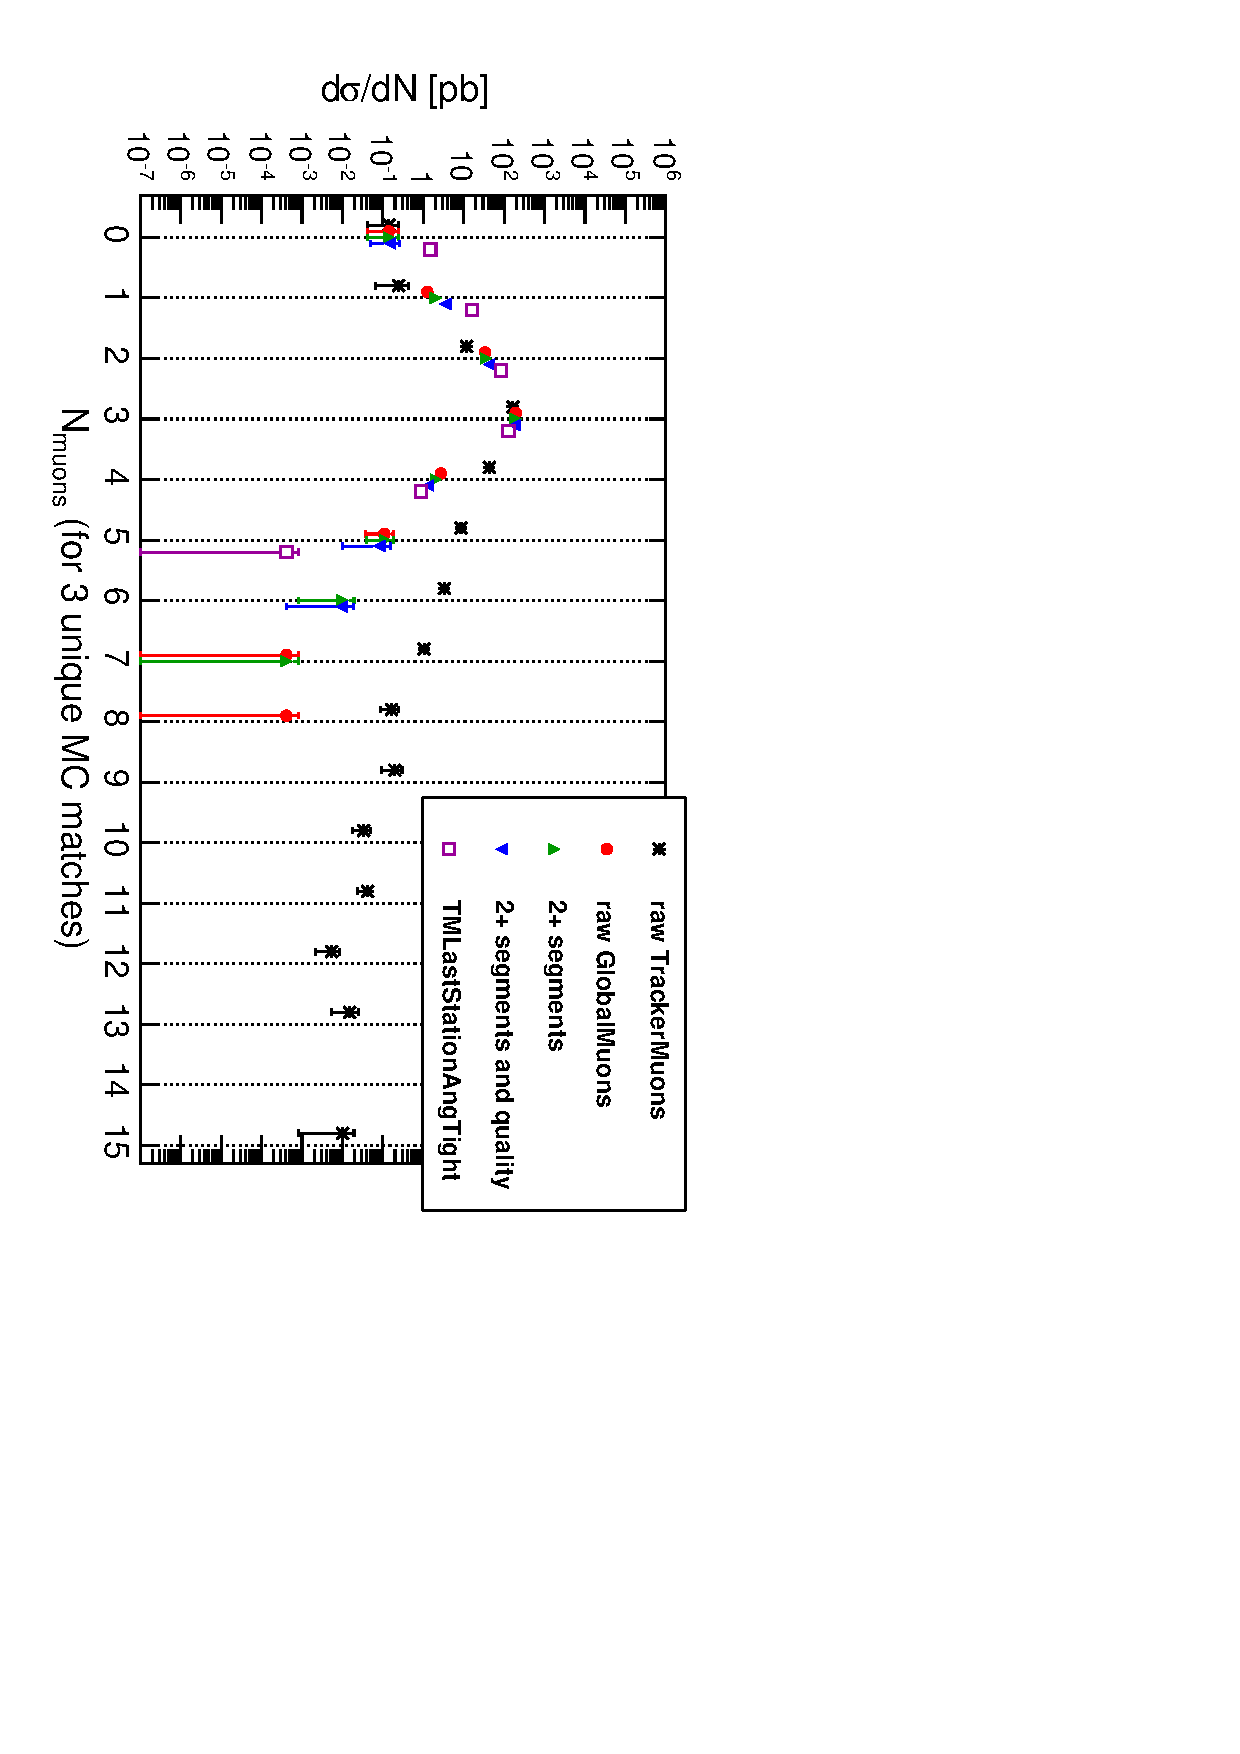
\includegraphics[height=0.5\linewidth, angle=90]{tracks_samepage_3real.pdf}
\end{frame}

\begin{frame}
\frametitle{Quality-TrackerMuon efficiency}

\begin{itemize}
\item Even with quality cuts and $N_\s{segments} \ge 2$, TrackerMuon
  efficiency is $\sim$95\% without a hard-to-model dip when pairs cross each other
\end{itemize}

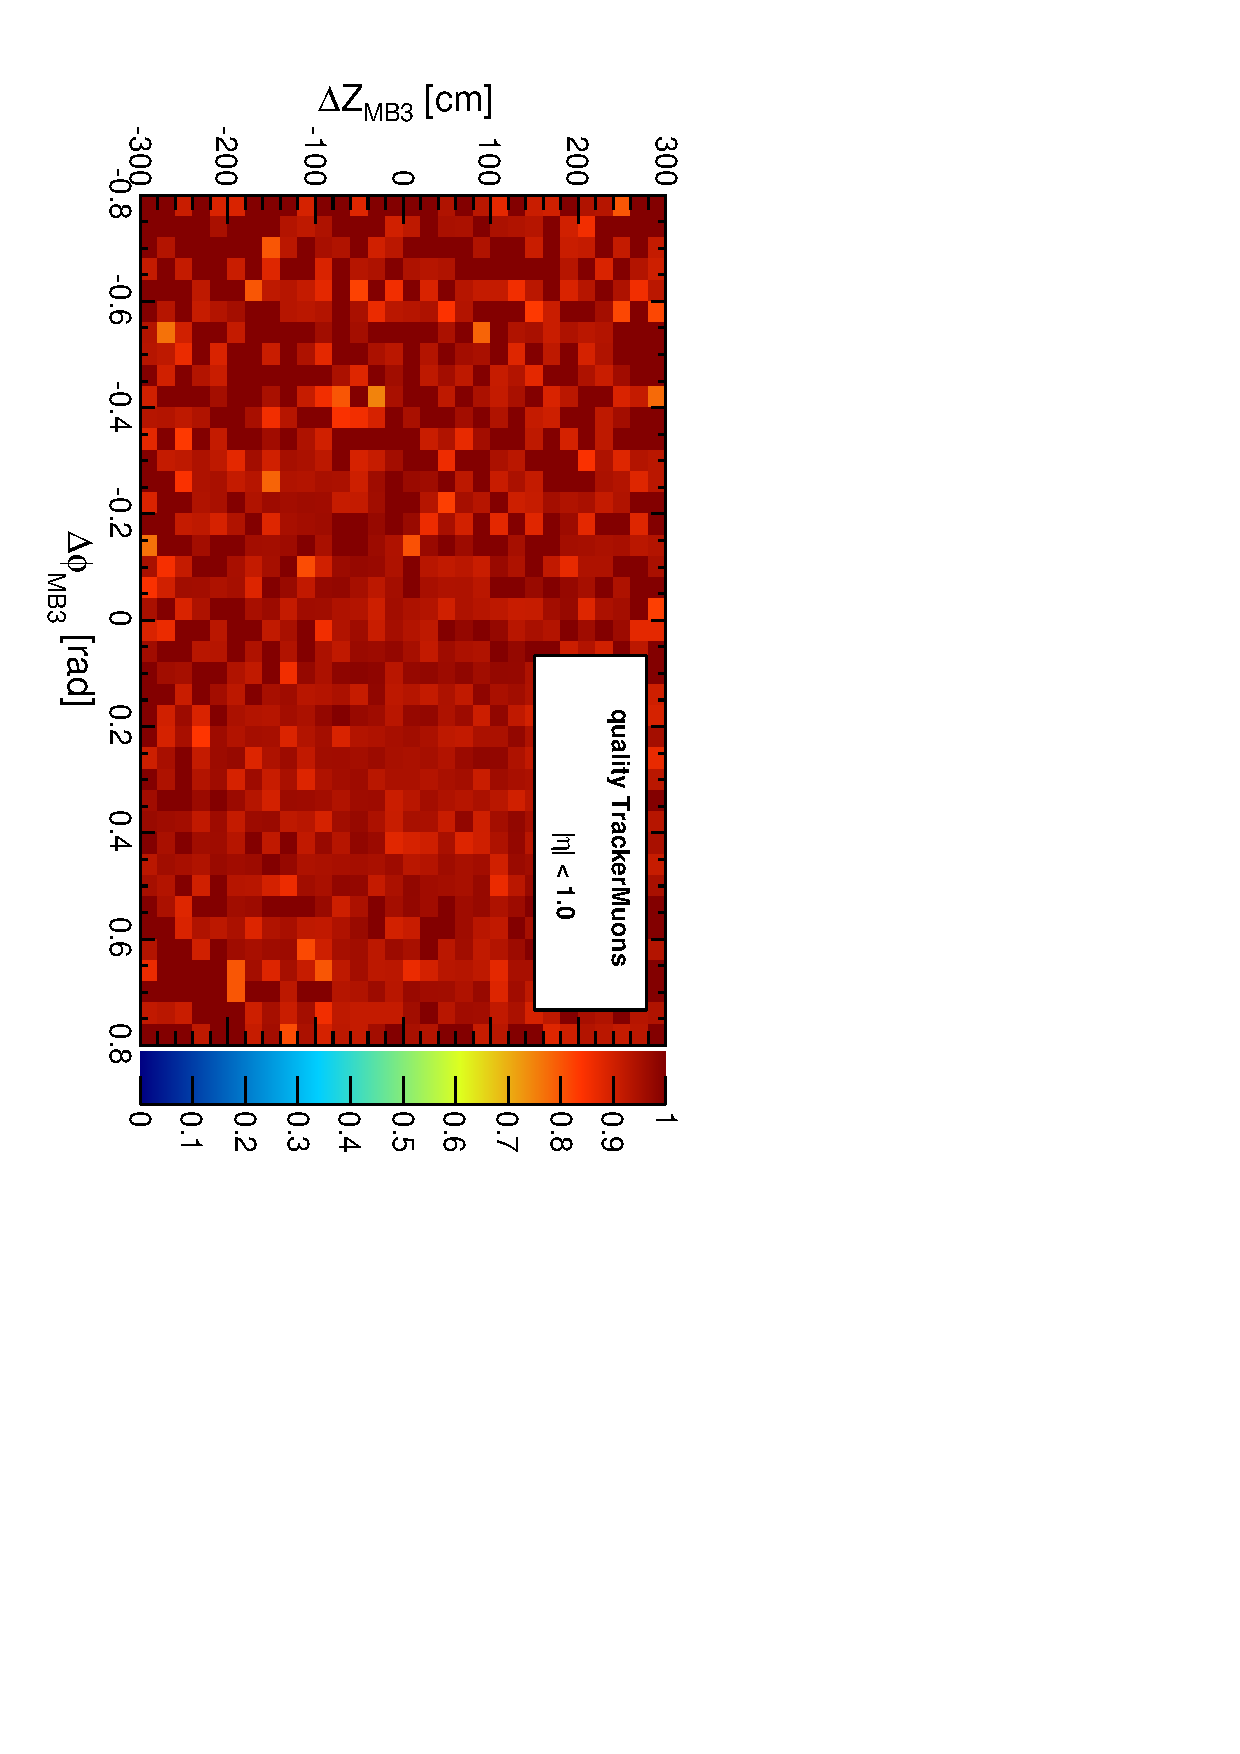
\includegraphics[height=0.5\linewidth, angle=90]{mb3_PlainTrackerMuon.pdf}
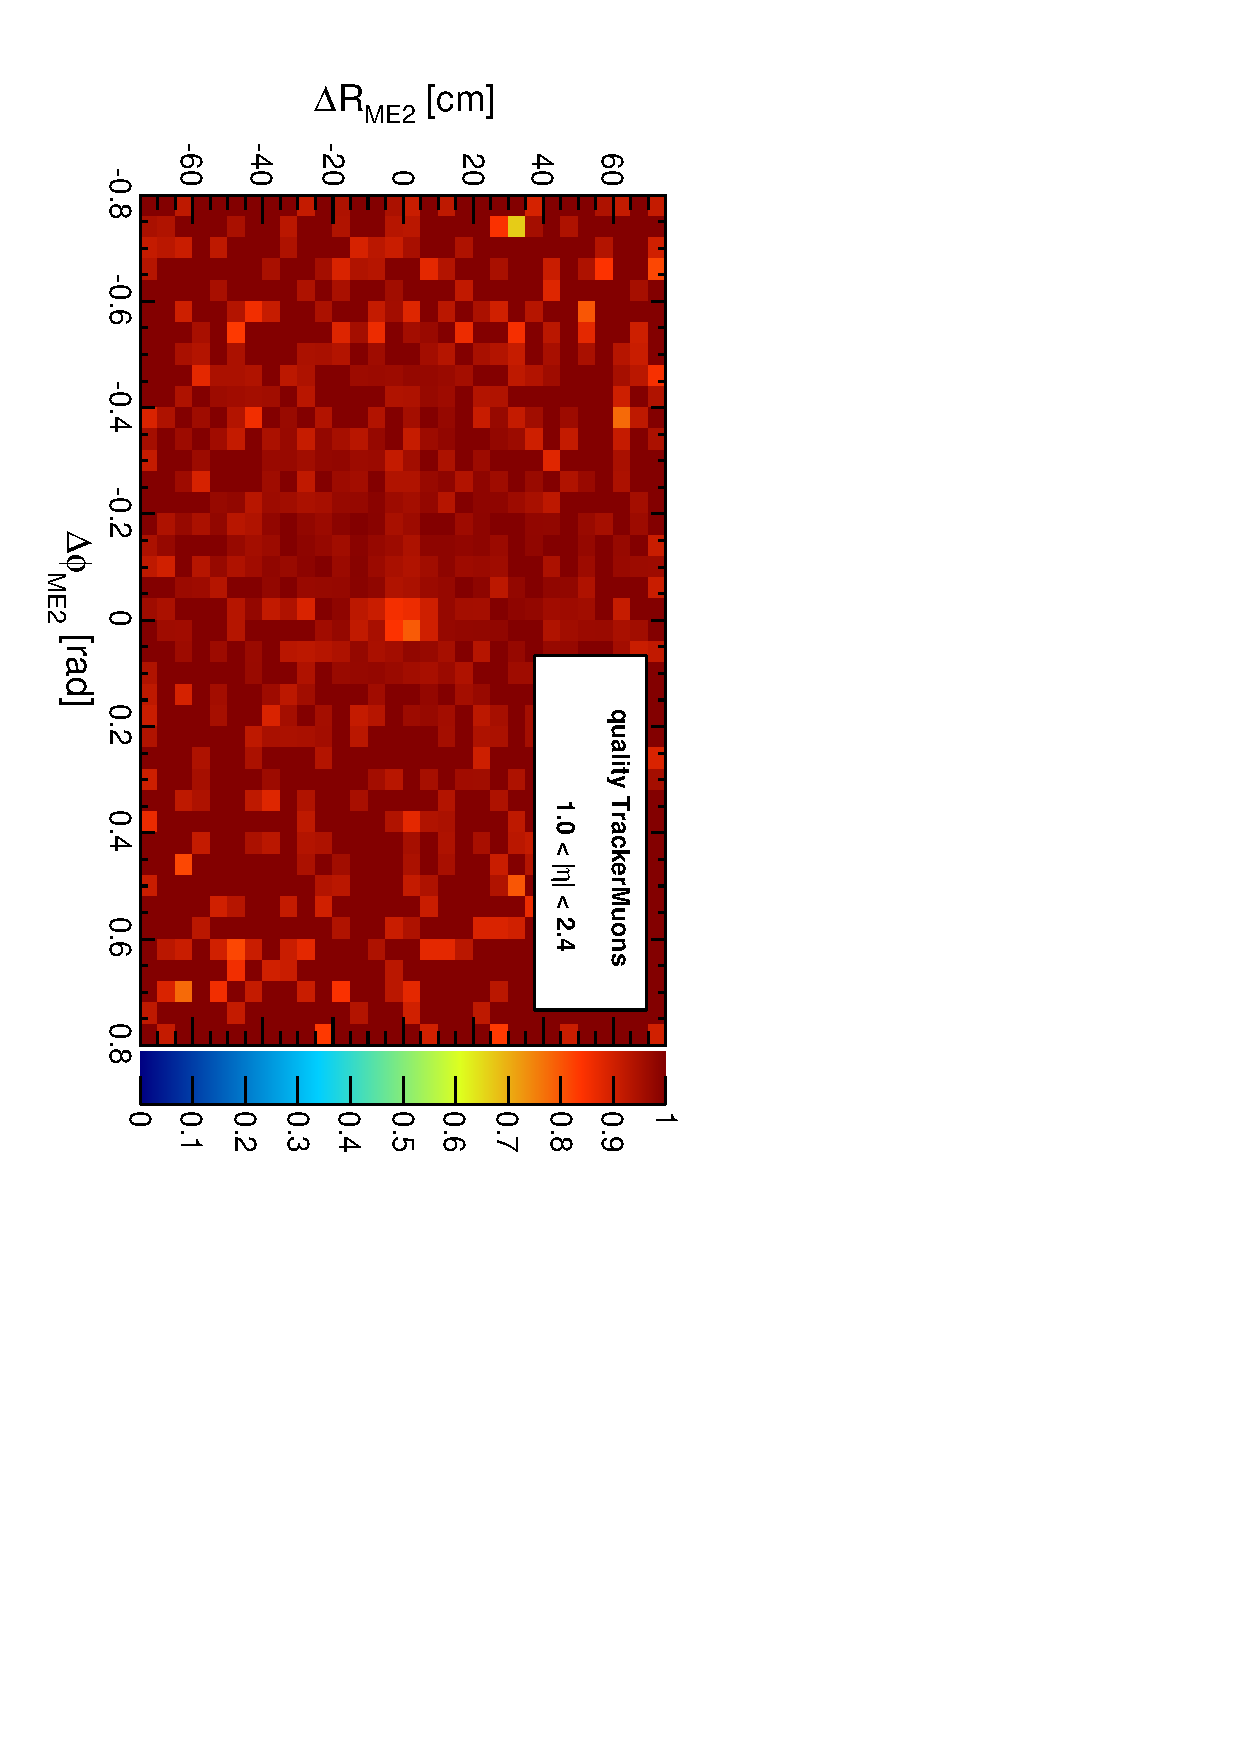
\includegraphics[height=0.5\linewidth, angle=90]{me2_PlainTrackerMuon.pdf}

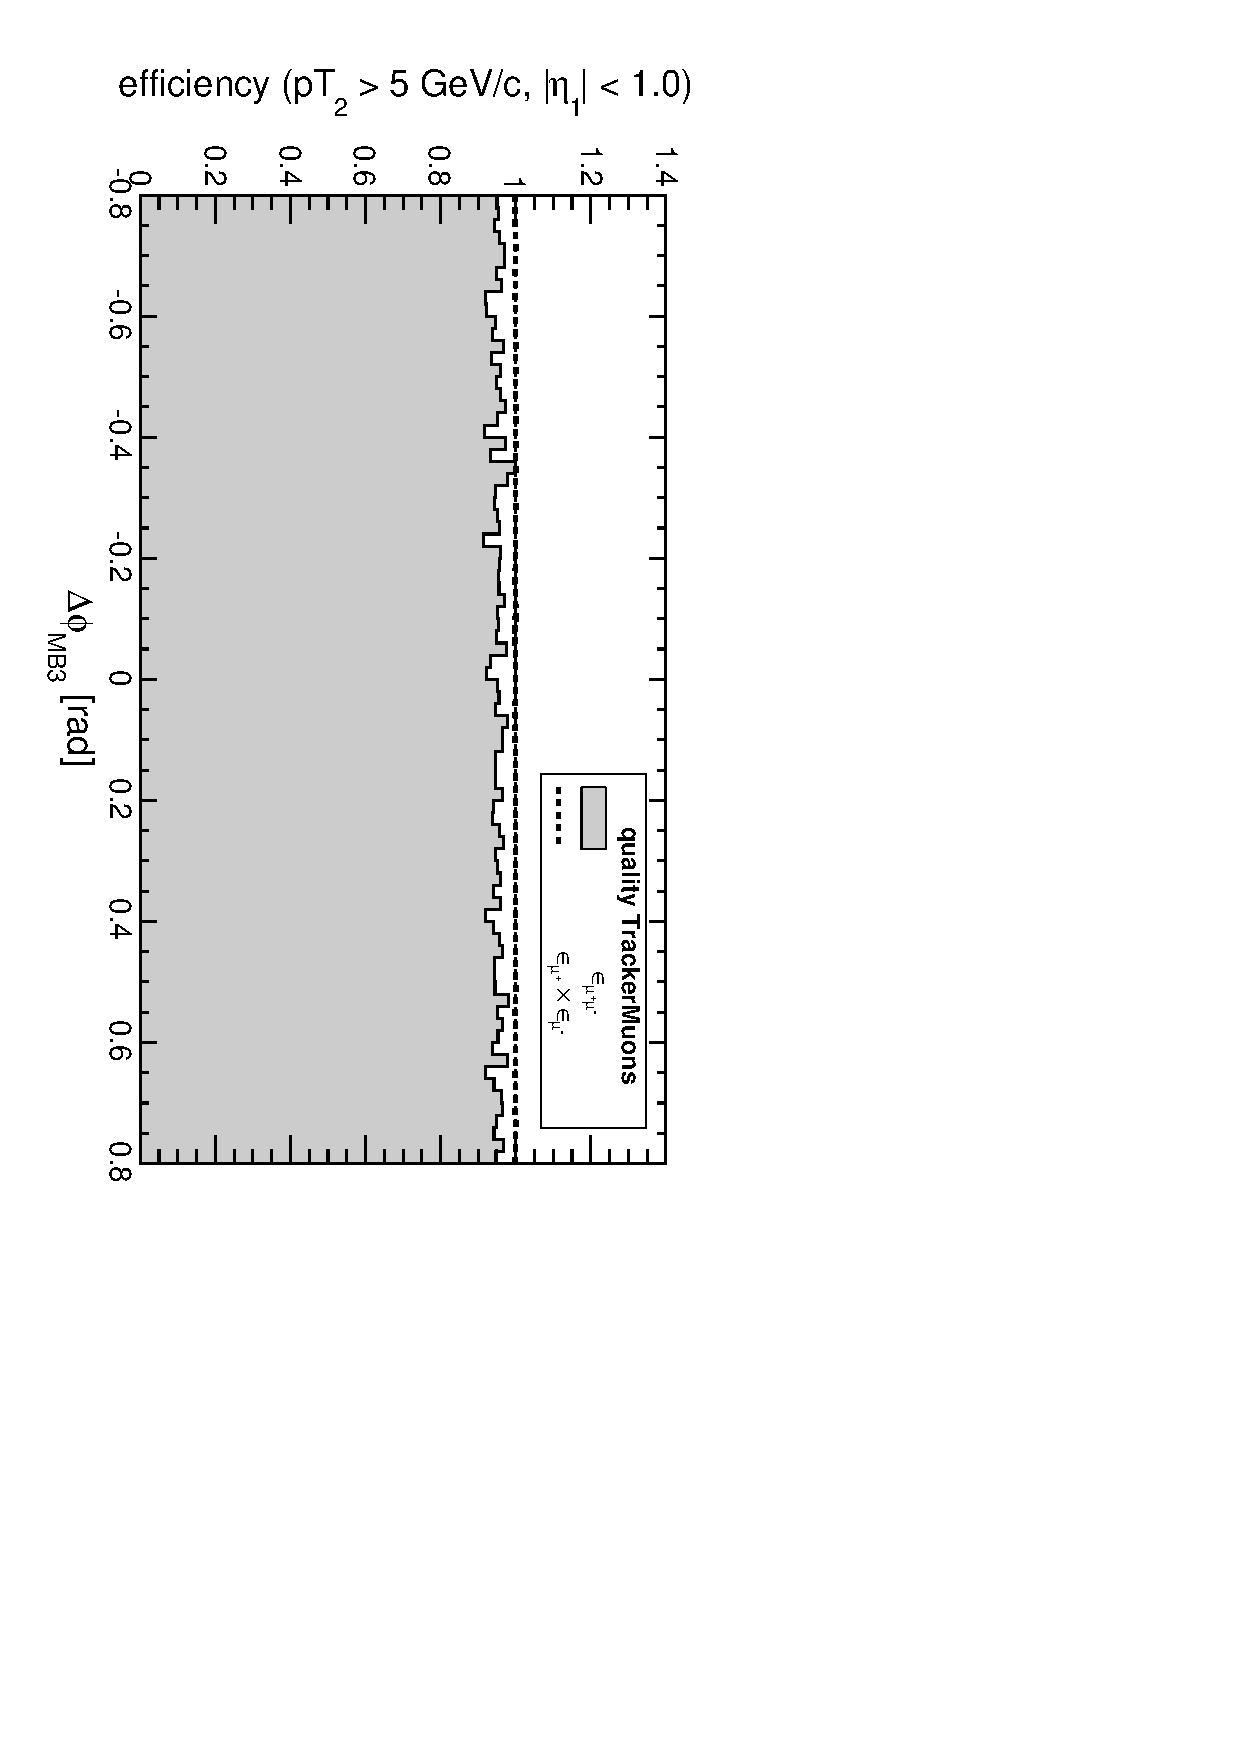
\includegraphics[height=0.5\linewidth, angle=90]{vsmb3dphi_PlainTrackerMuon.pdf}
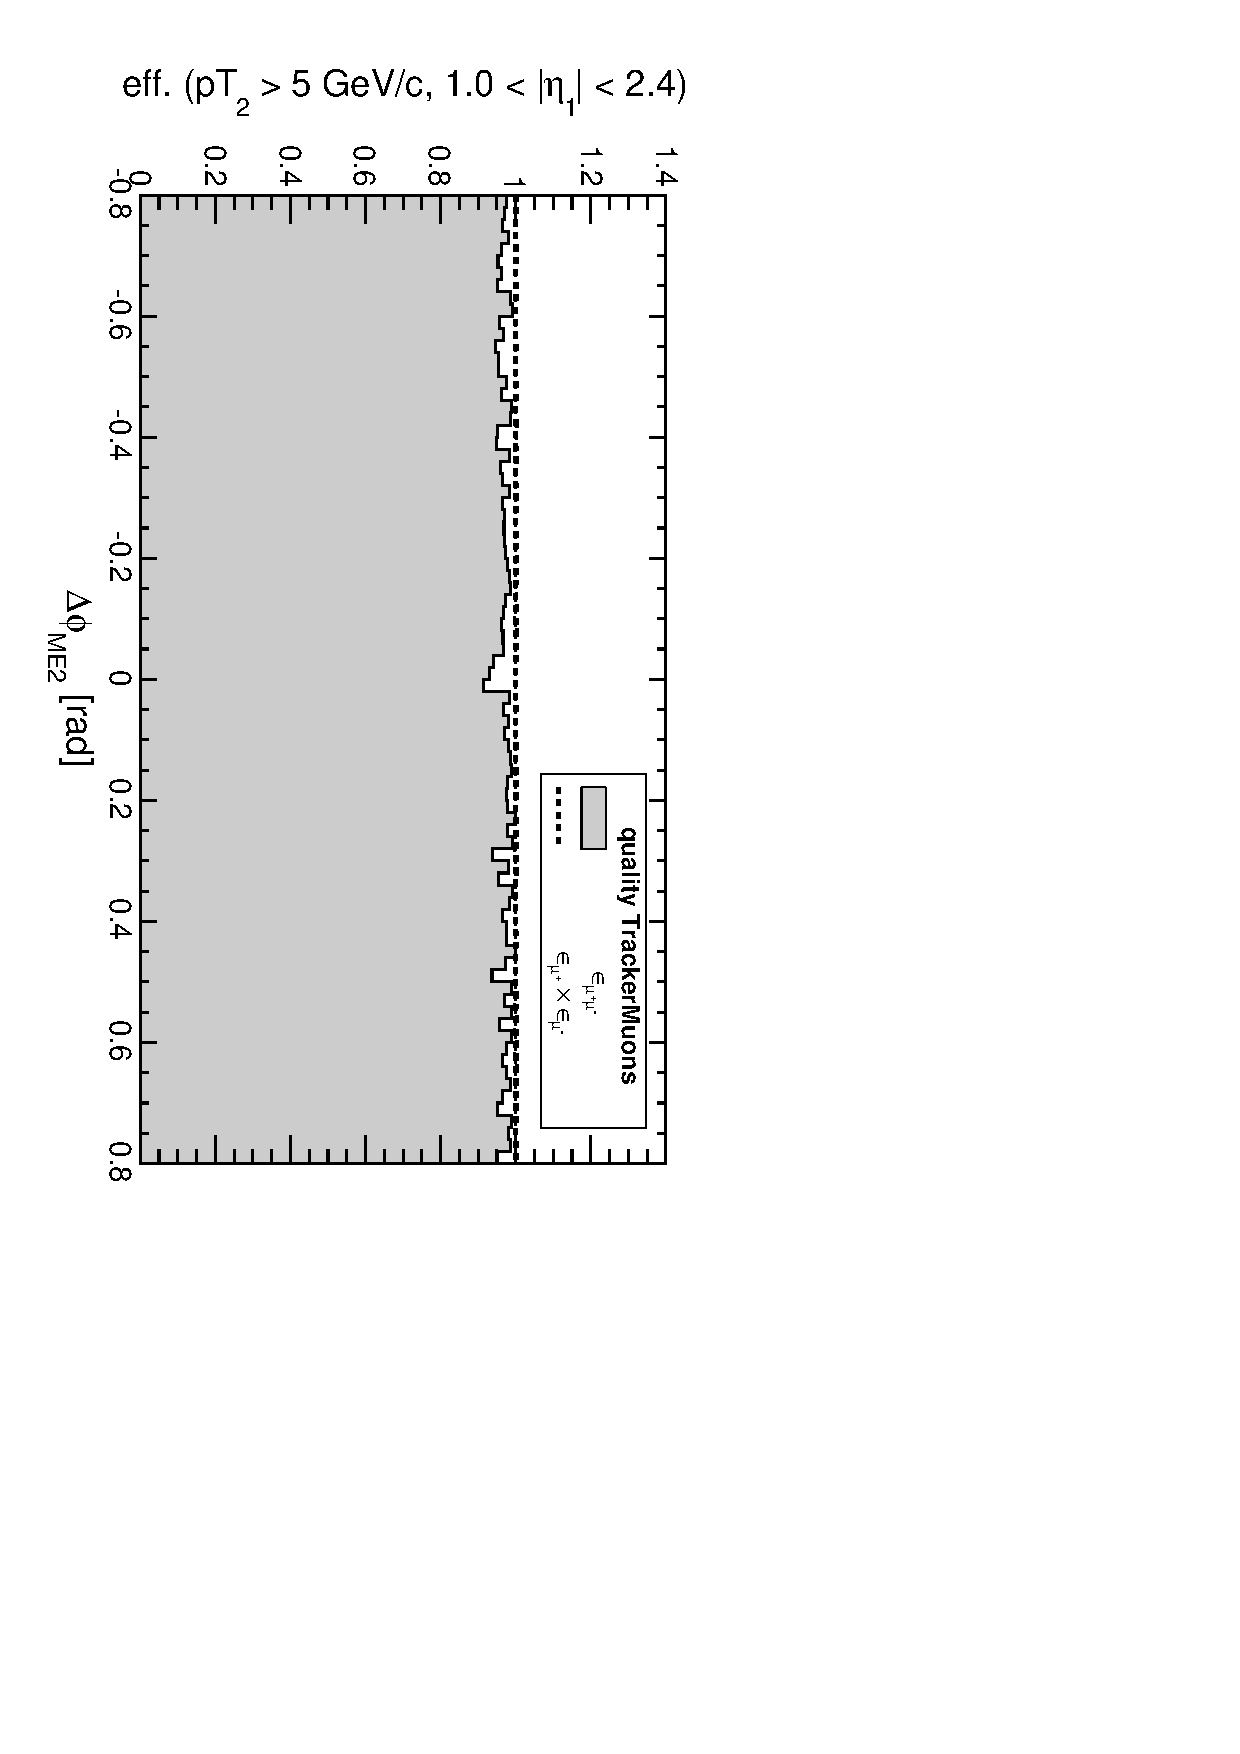
\includegraphics[height=0.5\linewidth, angle=90]{vsme2dphi_PlainTrackerMuon.pdf}
\end{frame}

\begin{frame}
\frametitle{Trigger efficiency}
\begin{itemize}
\item \textcolor{darkblue}{Significant issues in L1:}
\begin{itemize}
\item when multiple muons pass through the same chamber, only one may be read out
\item if an L1 muon is constructed from some $\mu^+$ segments and some $\mu^-$ segments, they may fail to be reconstructed as a single high-$p_T$ muon
\item this is not fully modeled in the L1 emulator!  (not for the CMSSW\_3\_6\_3 version that I'm using, anyway\ldots)
\end{itemize}
\item \textcolor{darkblue}{Significant issues in HLT:}
\begin{itemize}
\item uses StandAloneMuon reconstruction, with the inefficiencies I presented already
\item only need to reconstruct one StandAloneMuon at HLT, but reconstruction can be confused by overlaps
\end{itemize}
\item Also, time-dependence as trigger conditions change
\item I've made some basic trigger plots in MC, but the above must be
  addressed to meaningfully understand our trigger efficiencies
\end{itemize}
\end{frame}

\begin{frame}
\frametitle{QCD backgrounds: one $\mu$-group}

\begin{itemize}
\item The Standard Model has two clear signals in the one $\mu$-group
  channel: $J/\psi$ and $\phi(1020)$ (yellow)
\item $b \to c \to s$ with two semi-leptonic decays also correlates \mbox{muons (red)\hspace{-1 cm}}
\item<2> Only-one-muon (darker blue) suppressed with
  opposite-sign grouping
\end{itemize}

\only<1>{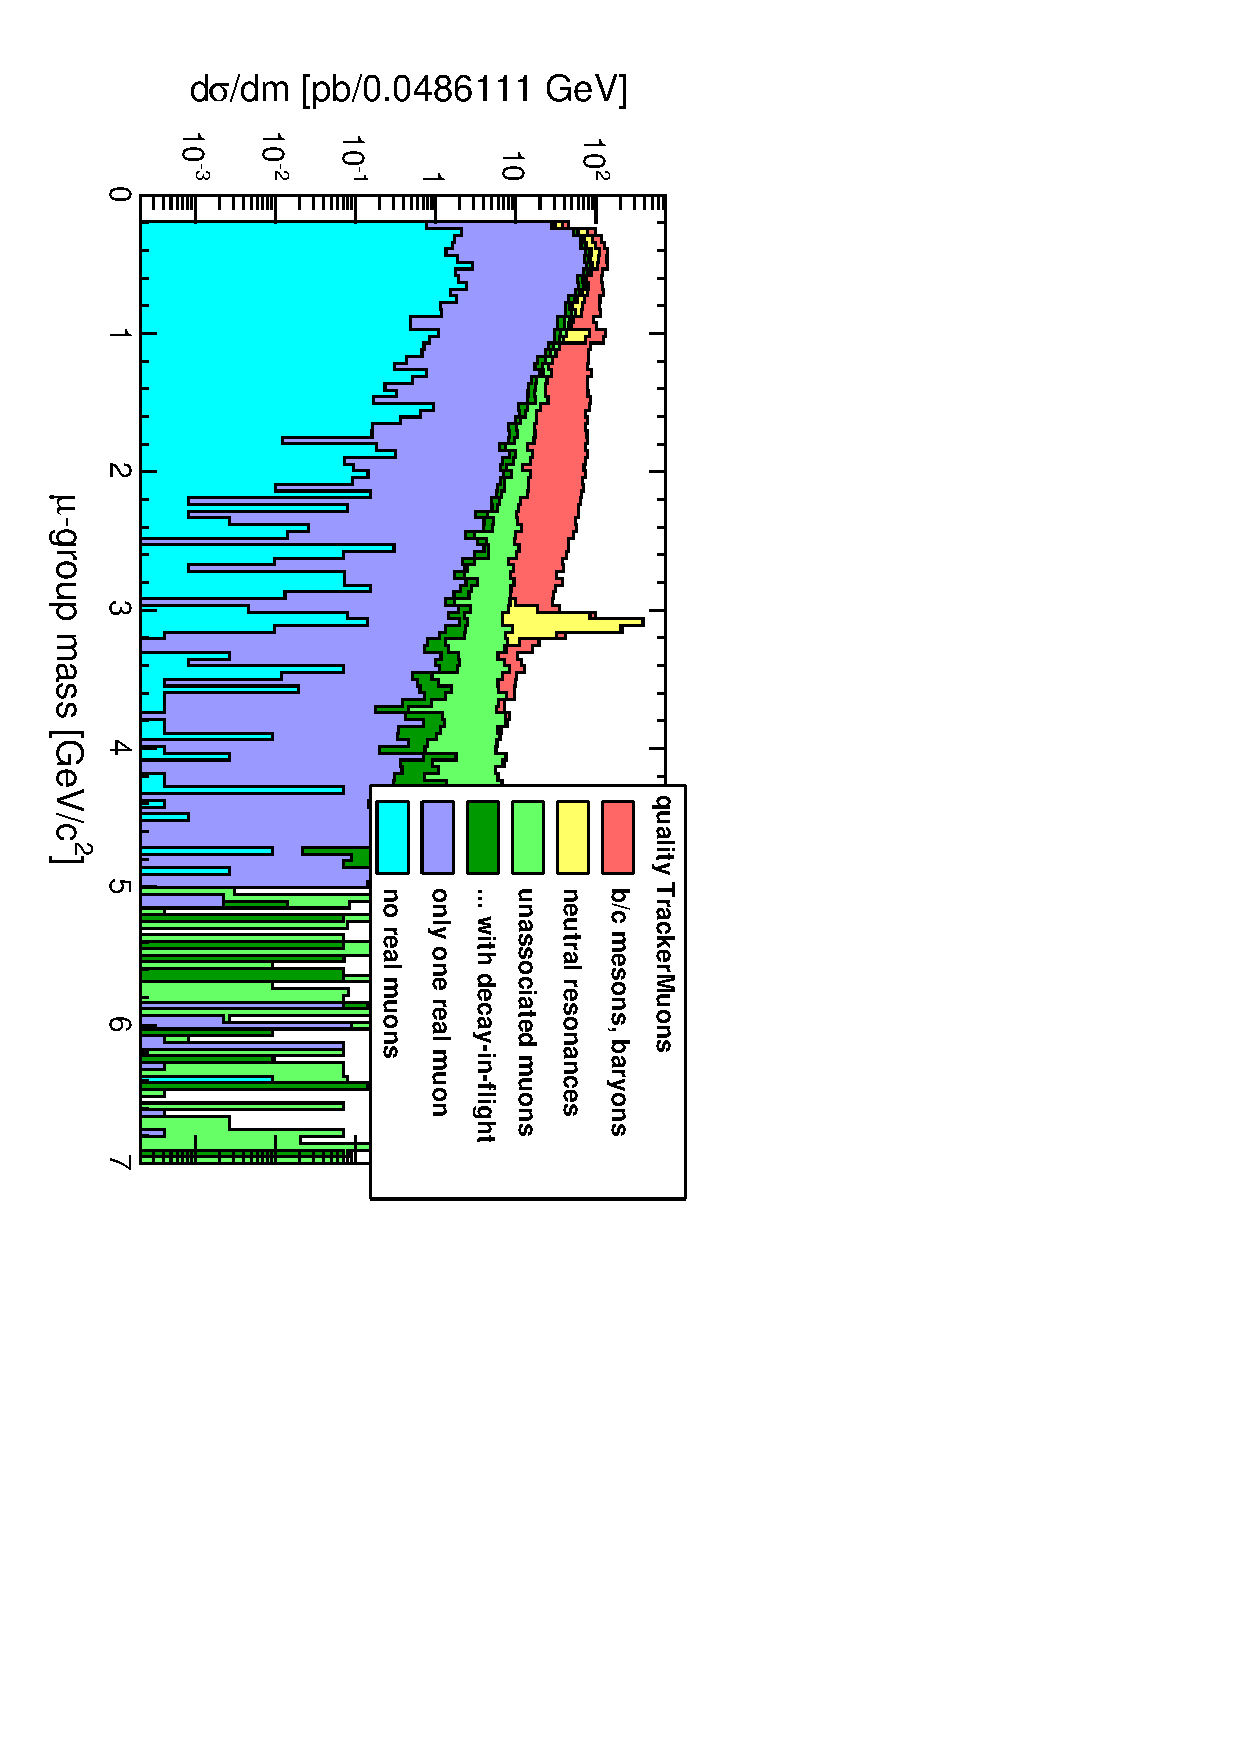
\includegraphics[height=0.5\linewidth, angle=90]{masslog_QualityTrackerMuonAny.pdf}
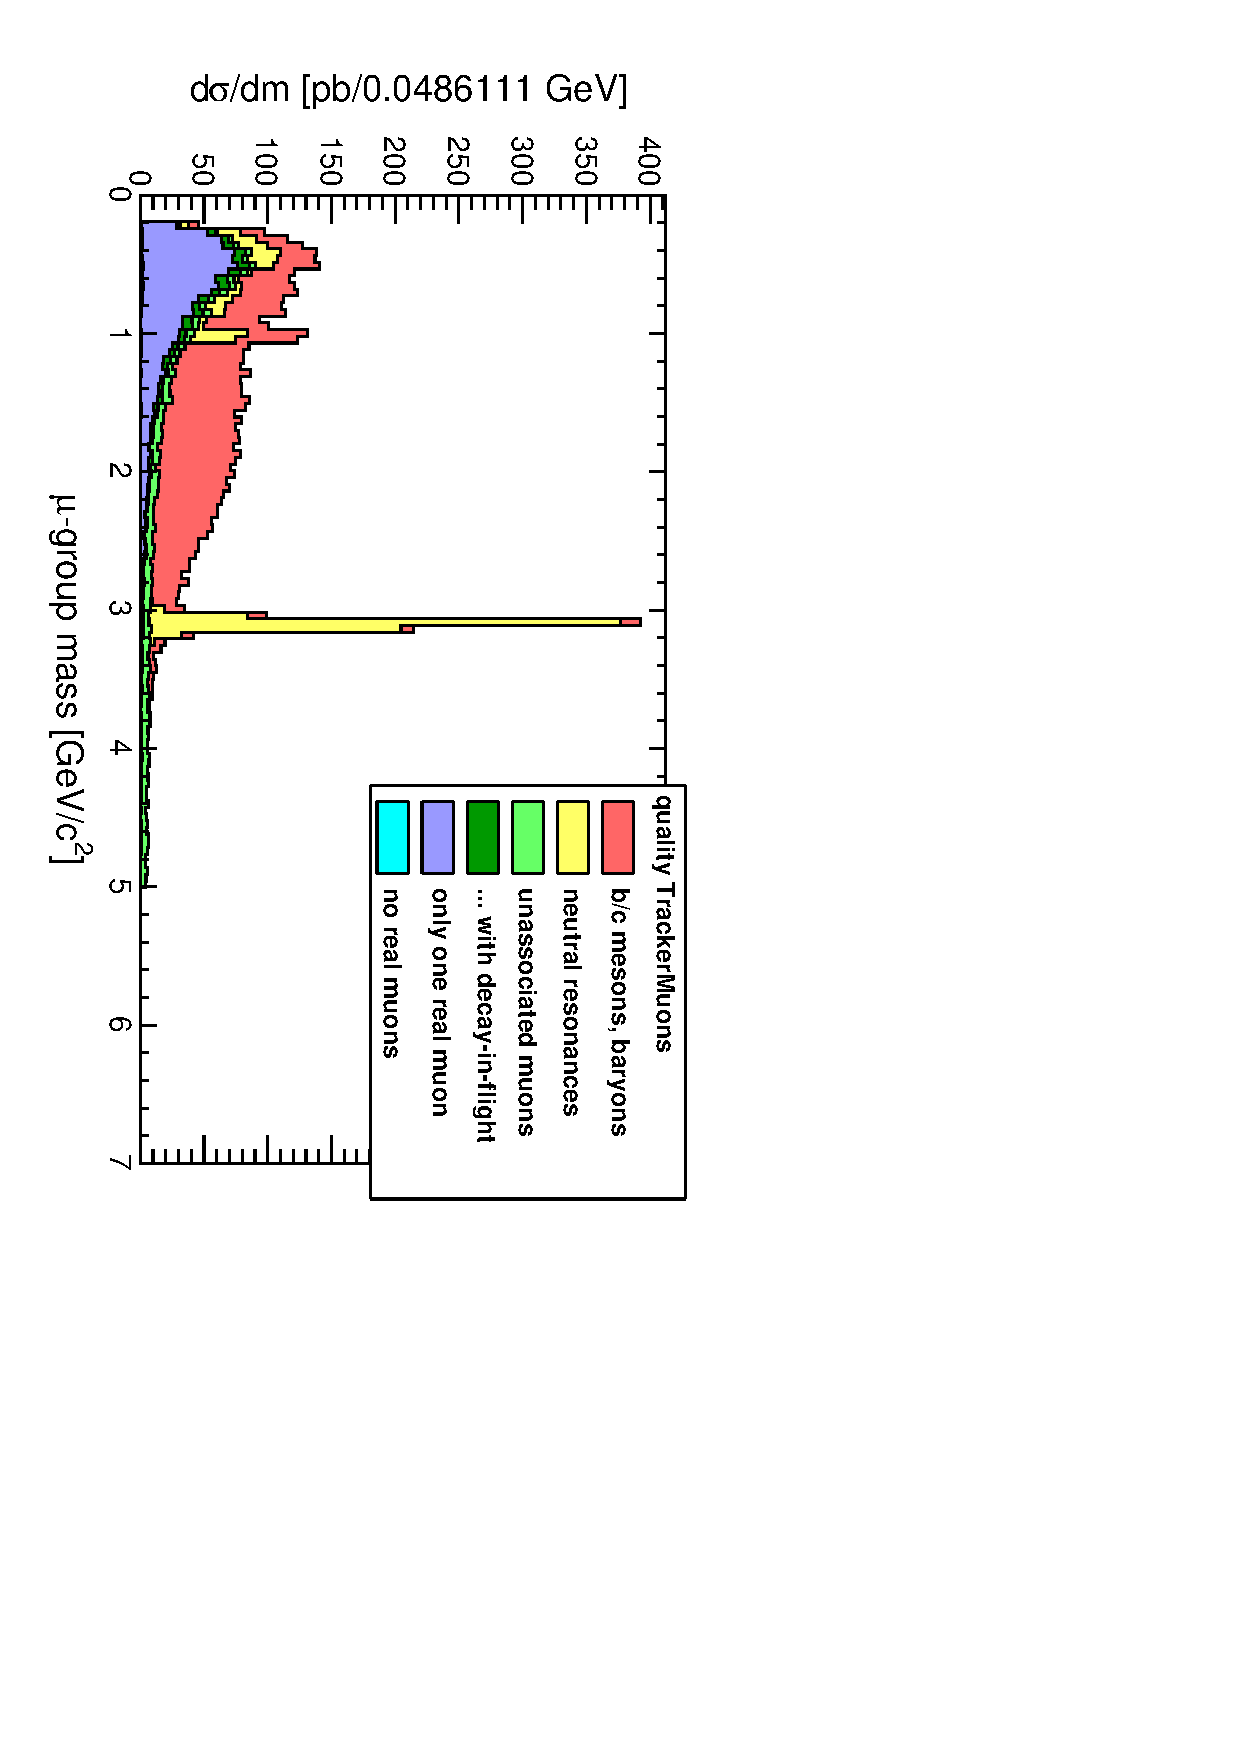
\includegraphics[height=0.5\linewidth, angle=90]{masslinear_QualityTrackerMuonAny.pdf}

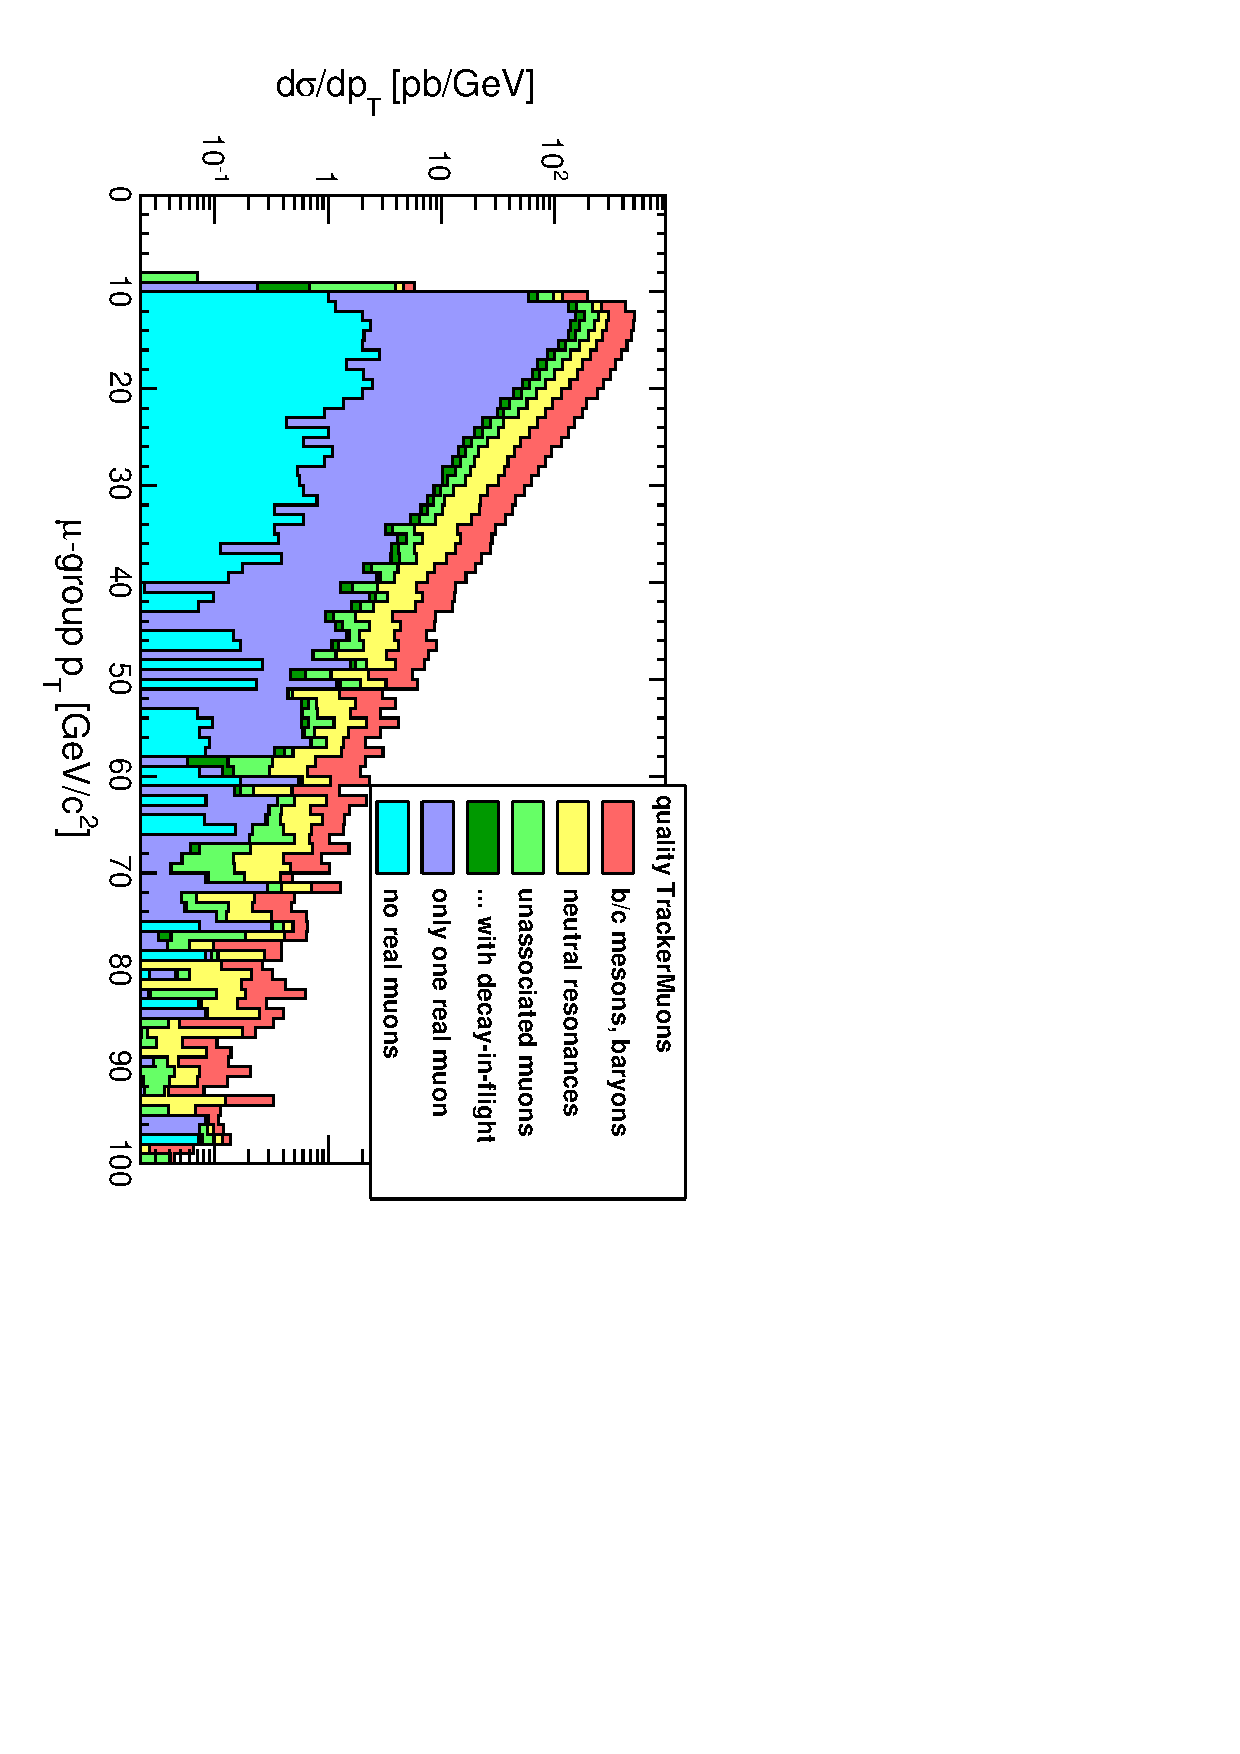
\includegraphics[height=0.5\linewidth, angle=90]{ptlog_QualityTrackerMuonAny.pdf}
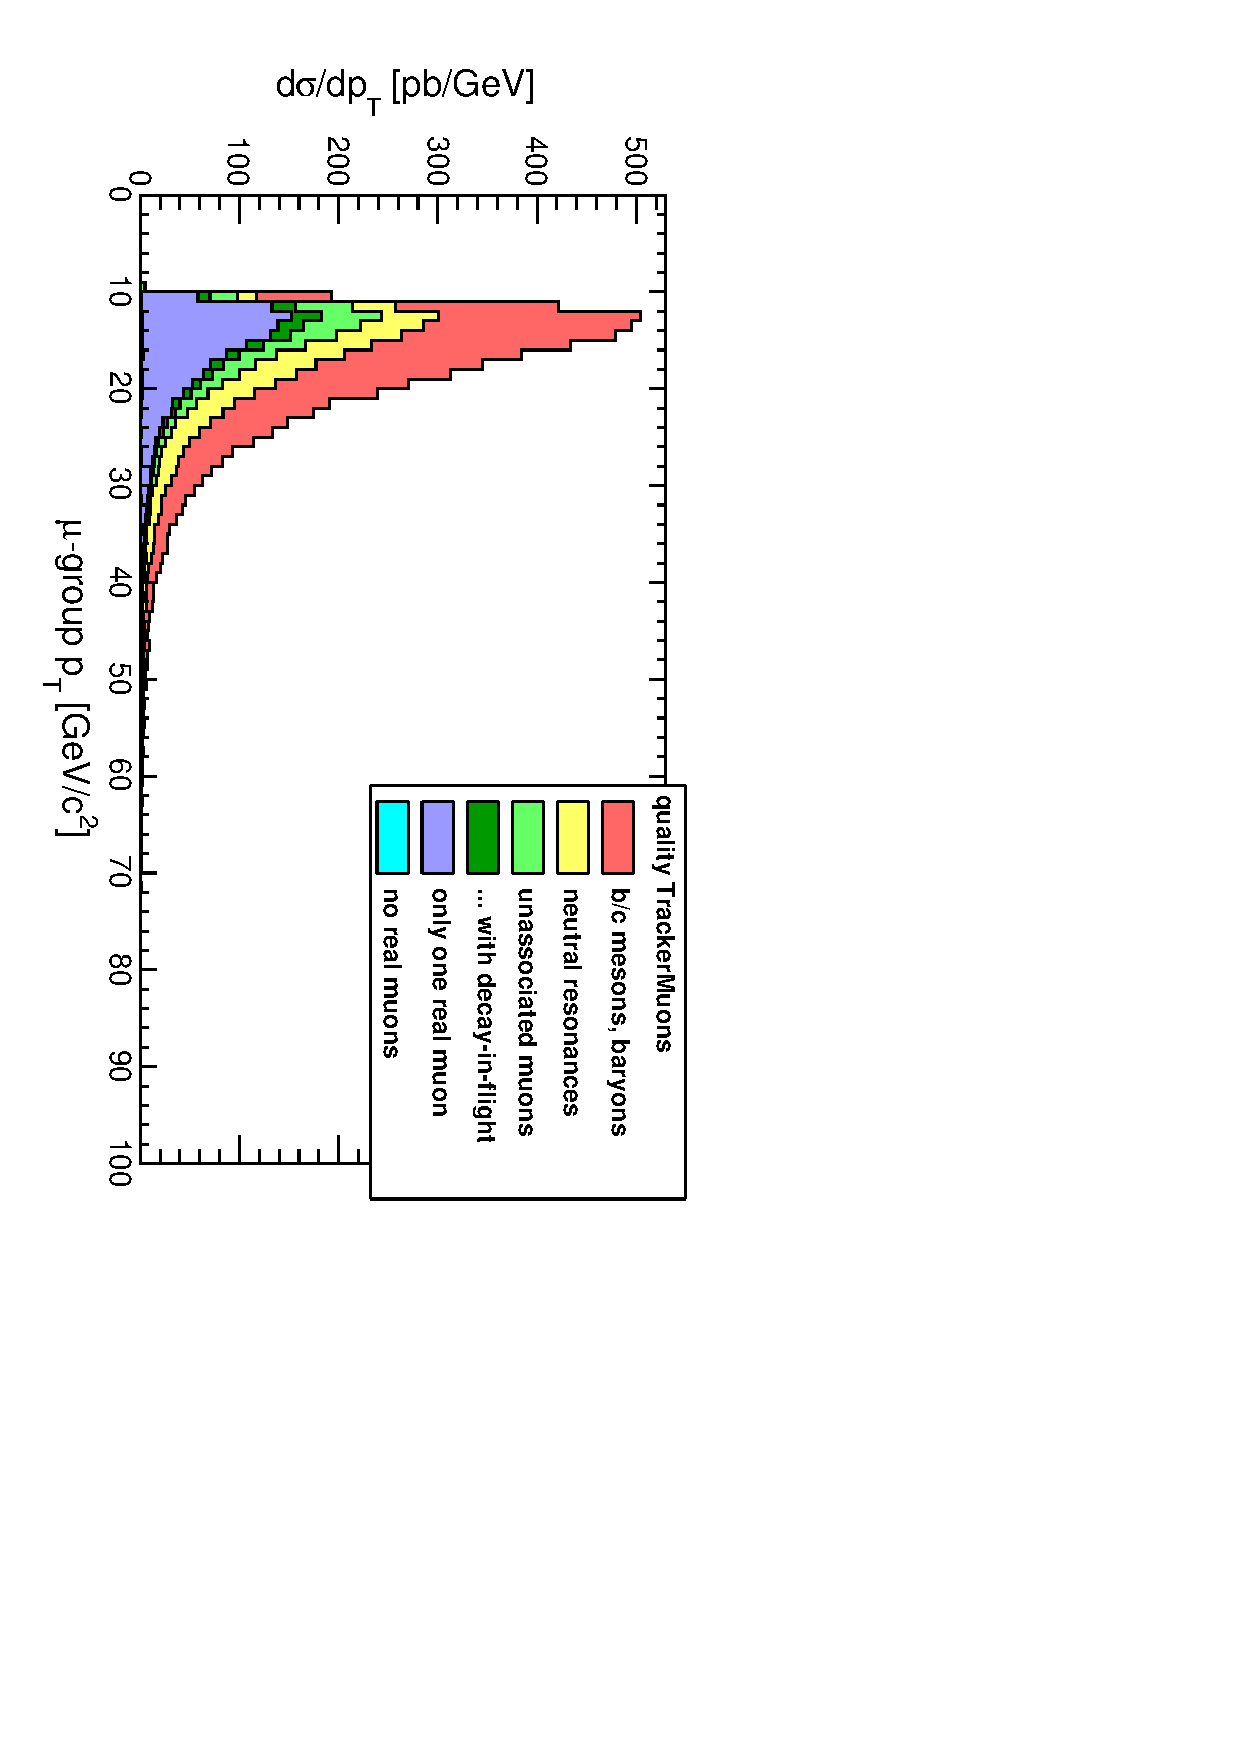
\includegraphics[height=0.5\linewidth, angle=90]{ptlinear_QualityTrackerMuonAny.pdf}}
\only<2>{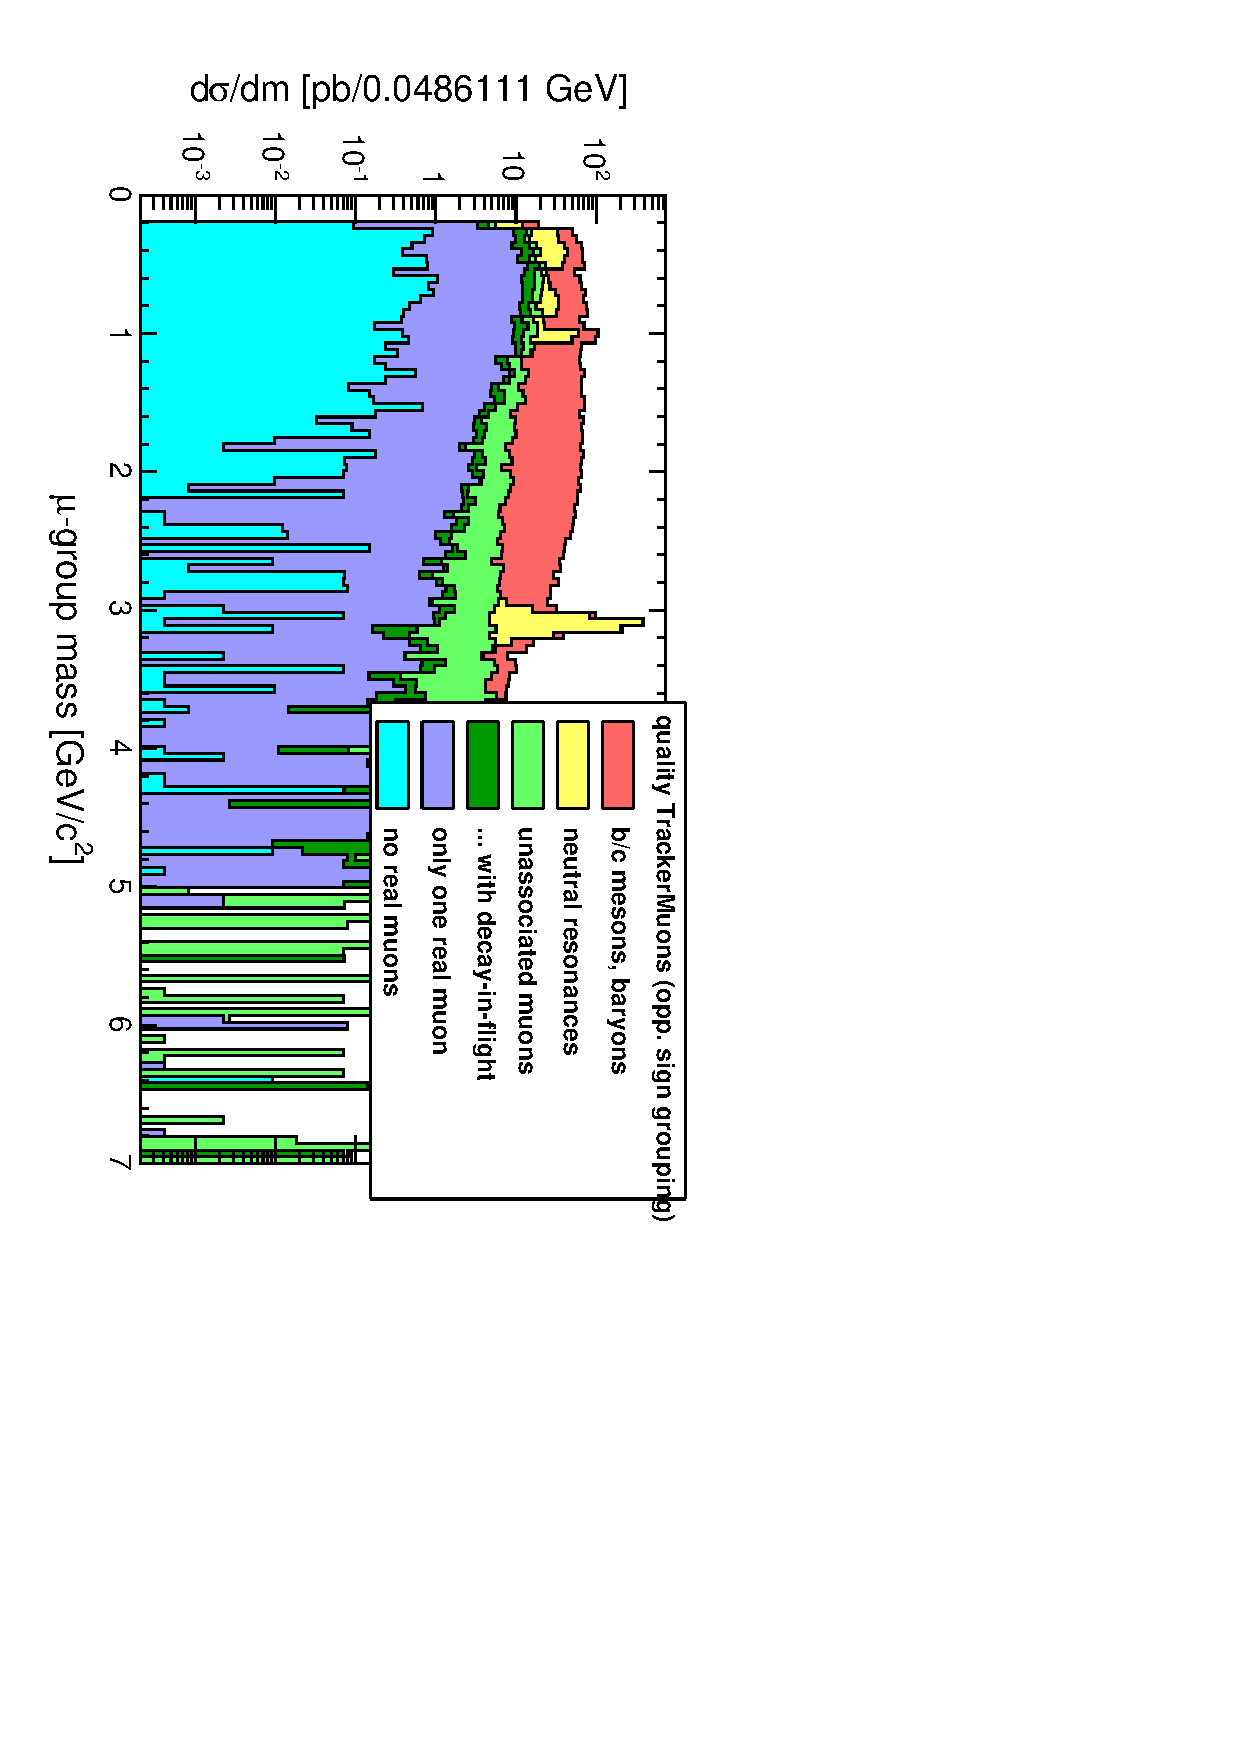
\includegraphics[height=0.5\linewidth, angle=90]{masslog_QualityTrackerMuonOpposite.pdf}
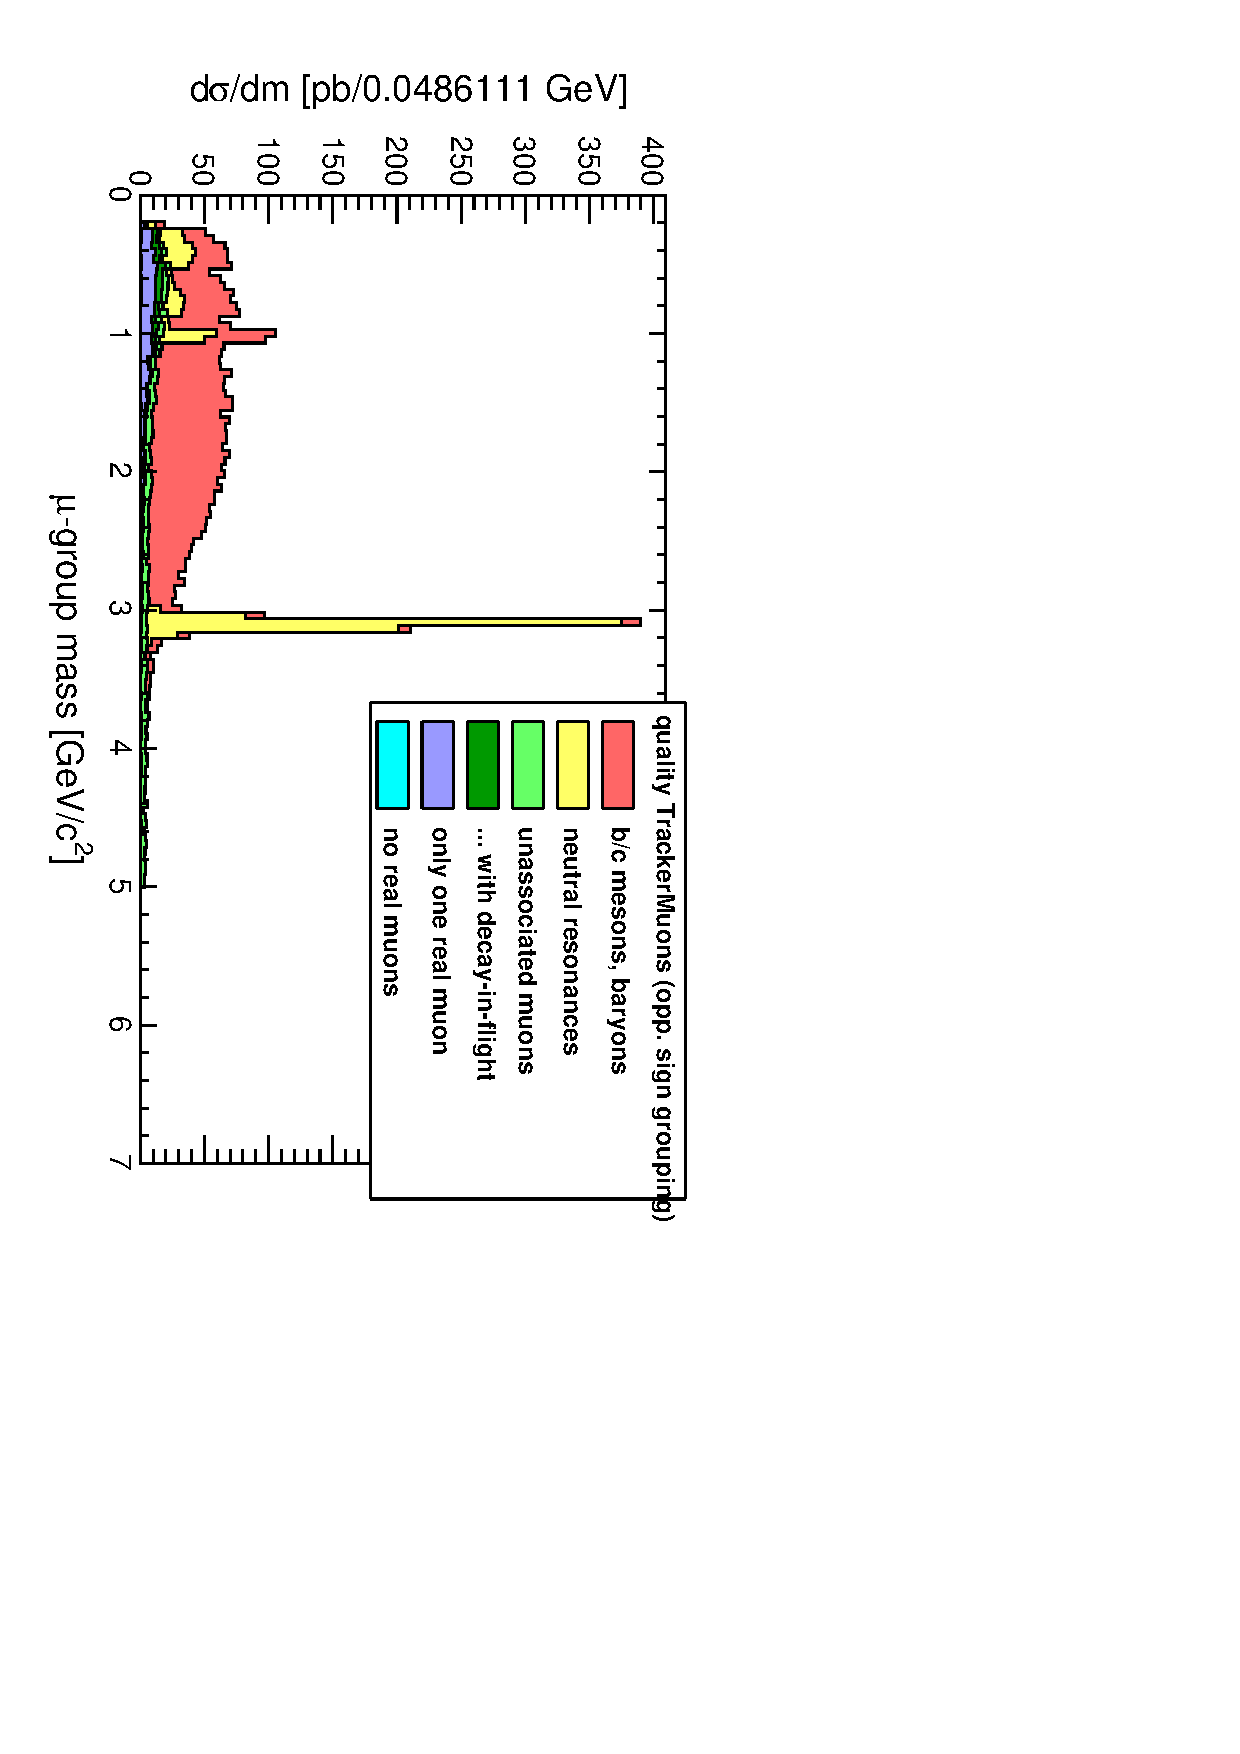
\includegraphics[height=0.5\linewidth, angle=90]{masslinear_QualityTrackerMuonOpposite.pdf}

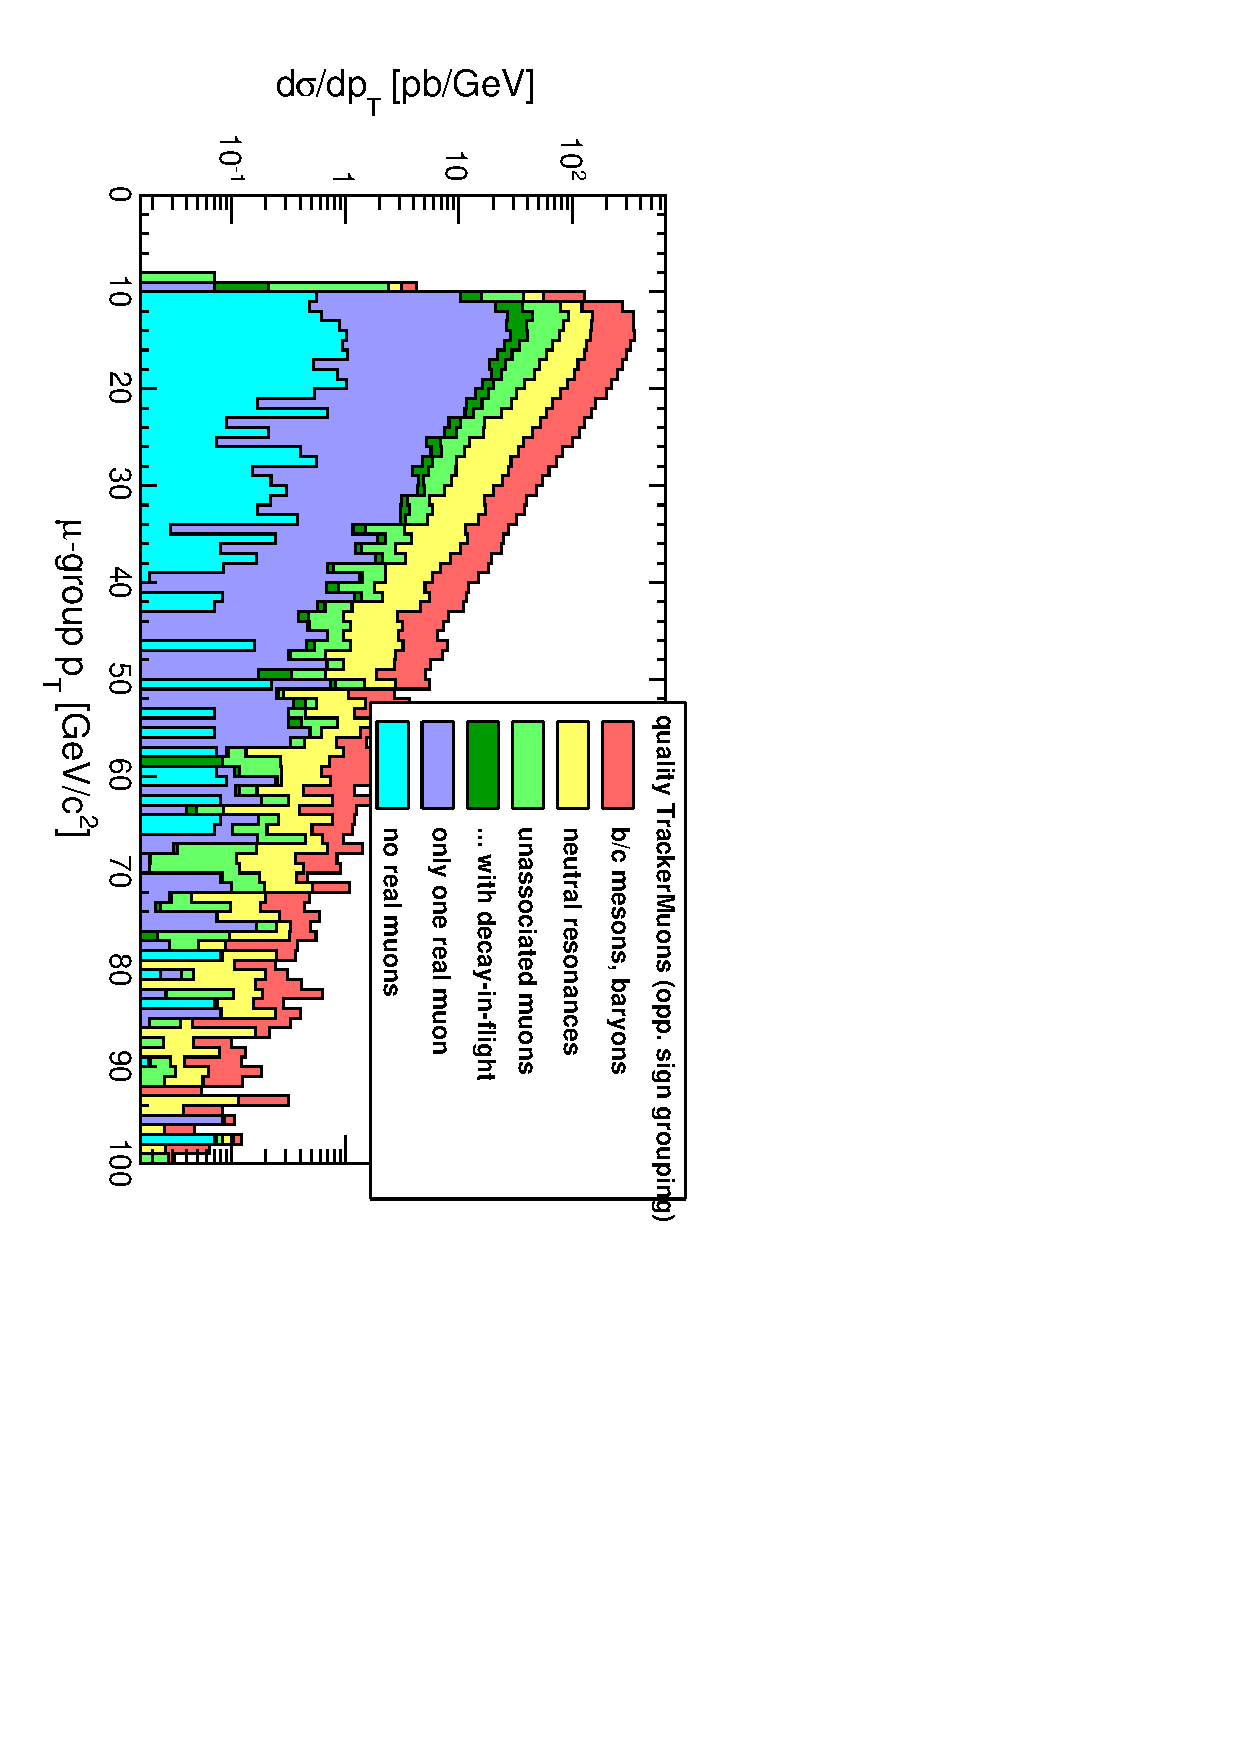
\includegraphics[height=0.5\linewidth, angle=90]{ptlog_QualityTrackerMuonOpposite.pdf}
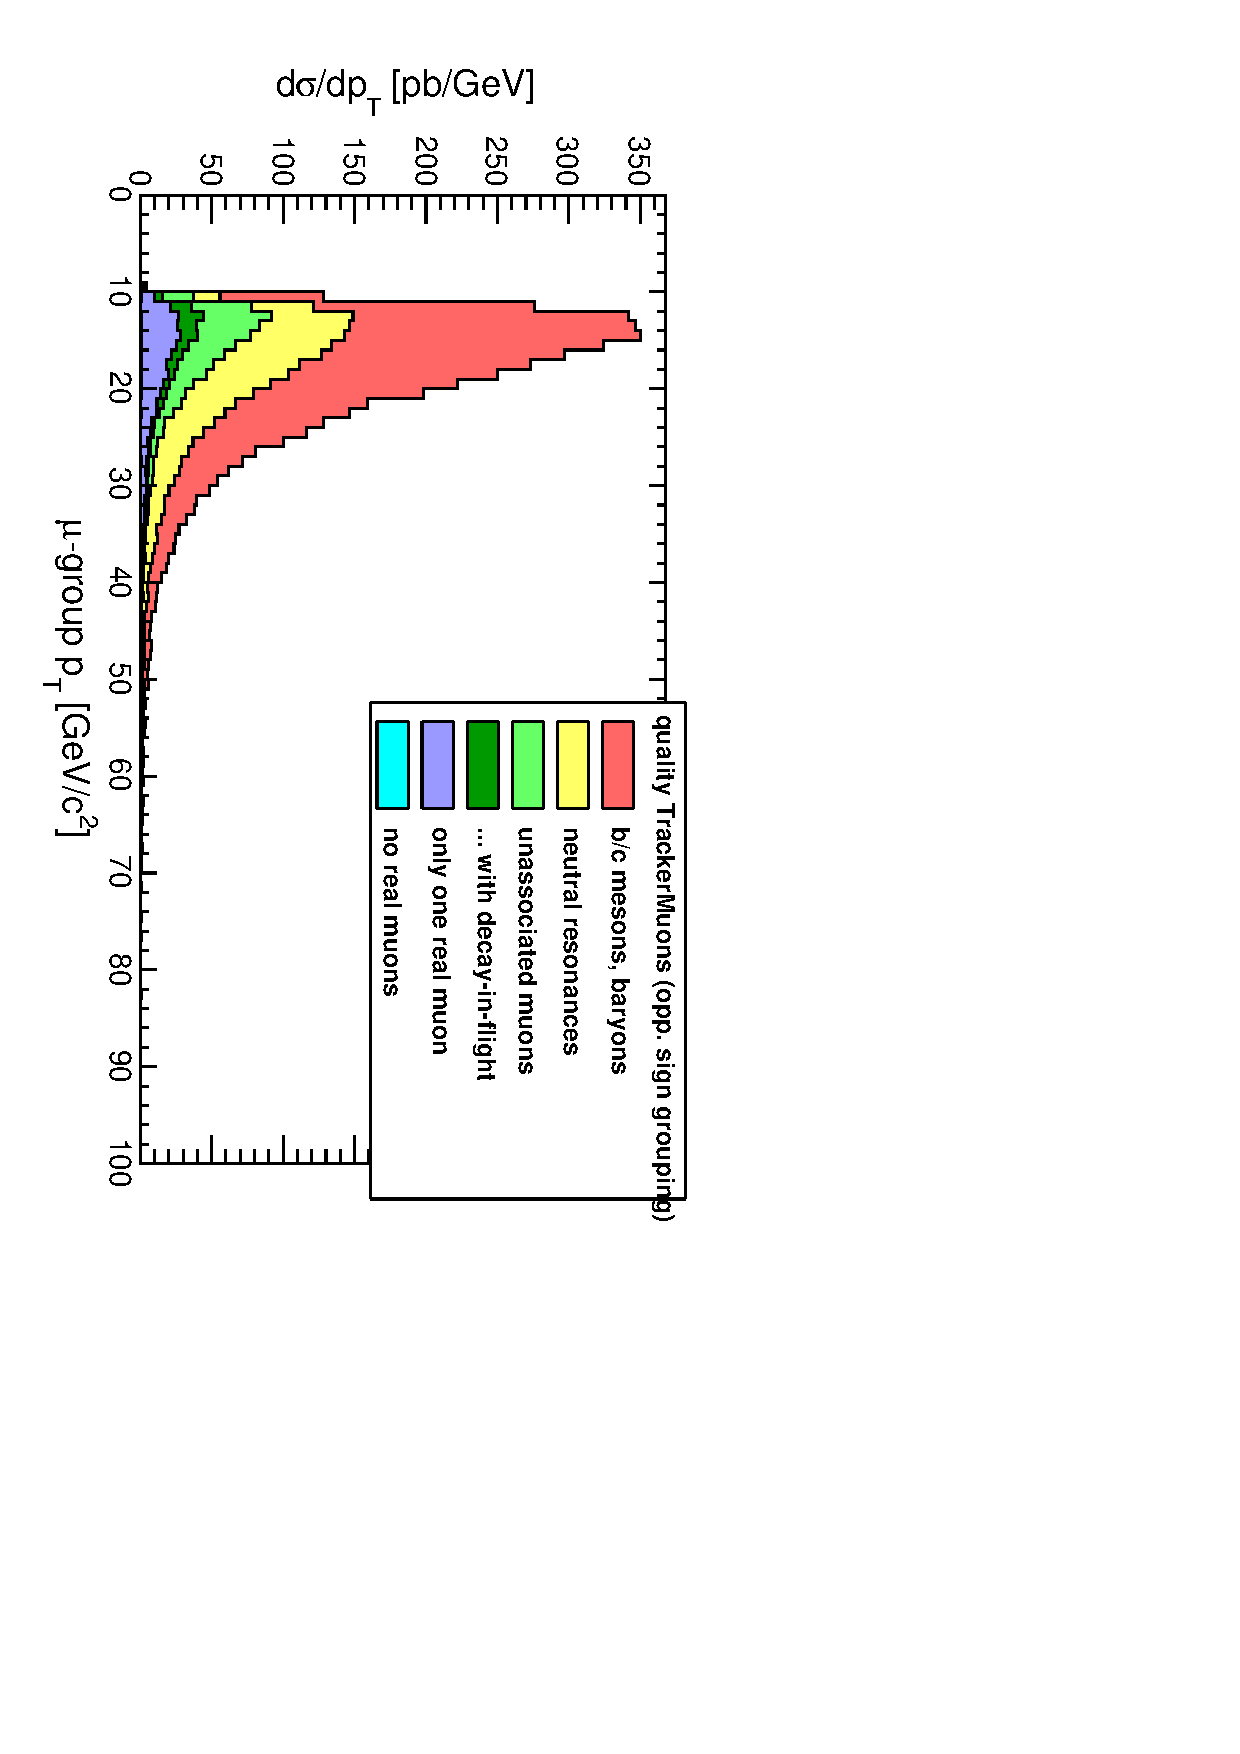
\includegraphics[height=0.5\linewidth, angle=90]{ptlinear_QualityTrackerMuonOpposite.pdf}}
\end{frame}

\begin{frame}
\frametitle{Multiple $\mu$-groups}

\begin{itemize}
\item Asking for a second $\mu$-group reduces the QCD backgrounds to 1~pb
\item Many of the models we've looked at have $\sim$pb cross-sections or at least limits can be set with 1--100~pb$^{-1}$
\item Since we're looking for new resonances, we get more sensitivity
  by searching for peaks: the QCD backgrounds are roughly flat in mass
\end{itemize}

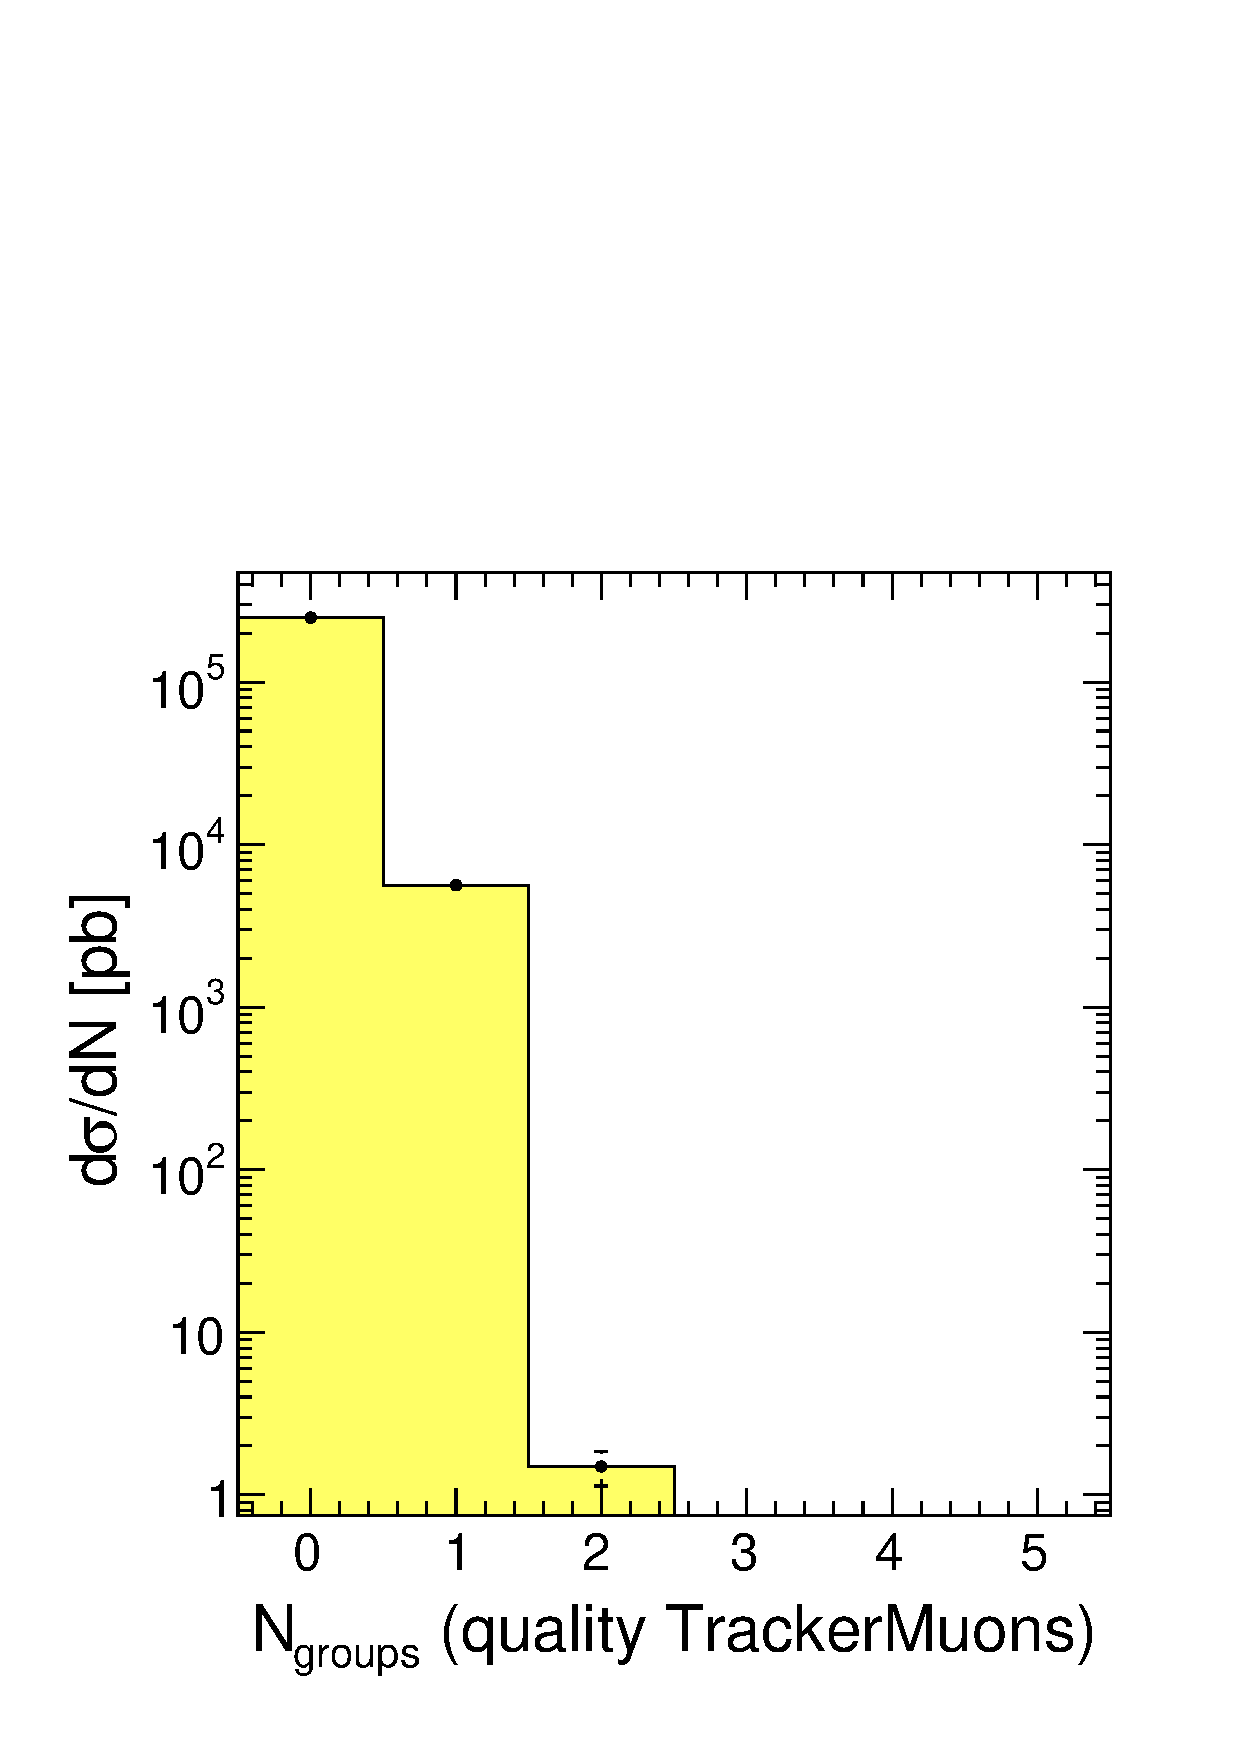
\includegraphics[height=4 cm]{groups_QualityTrackerMuonAny.pdf}
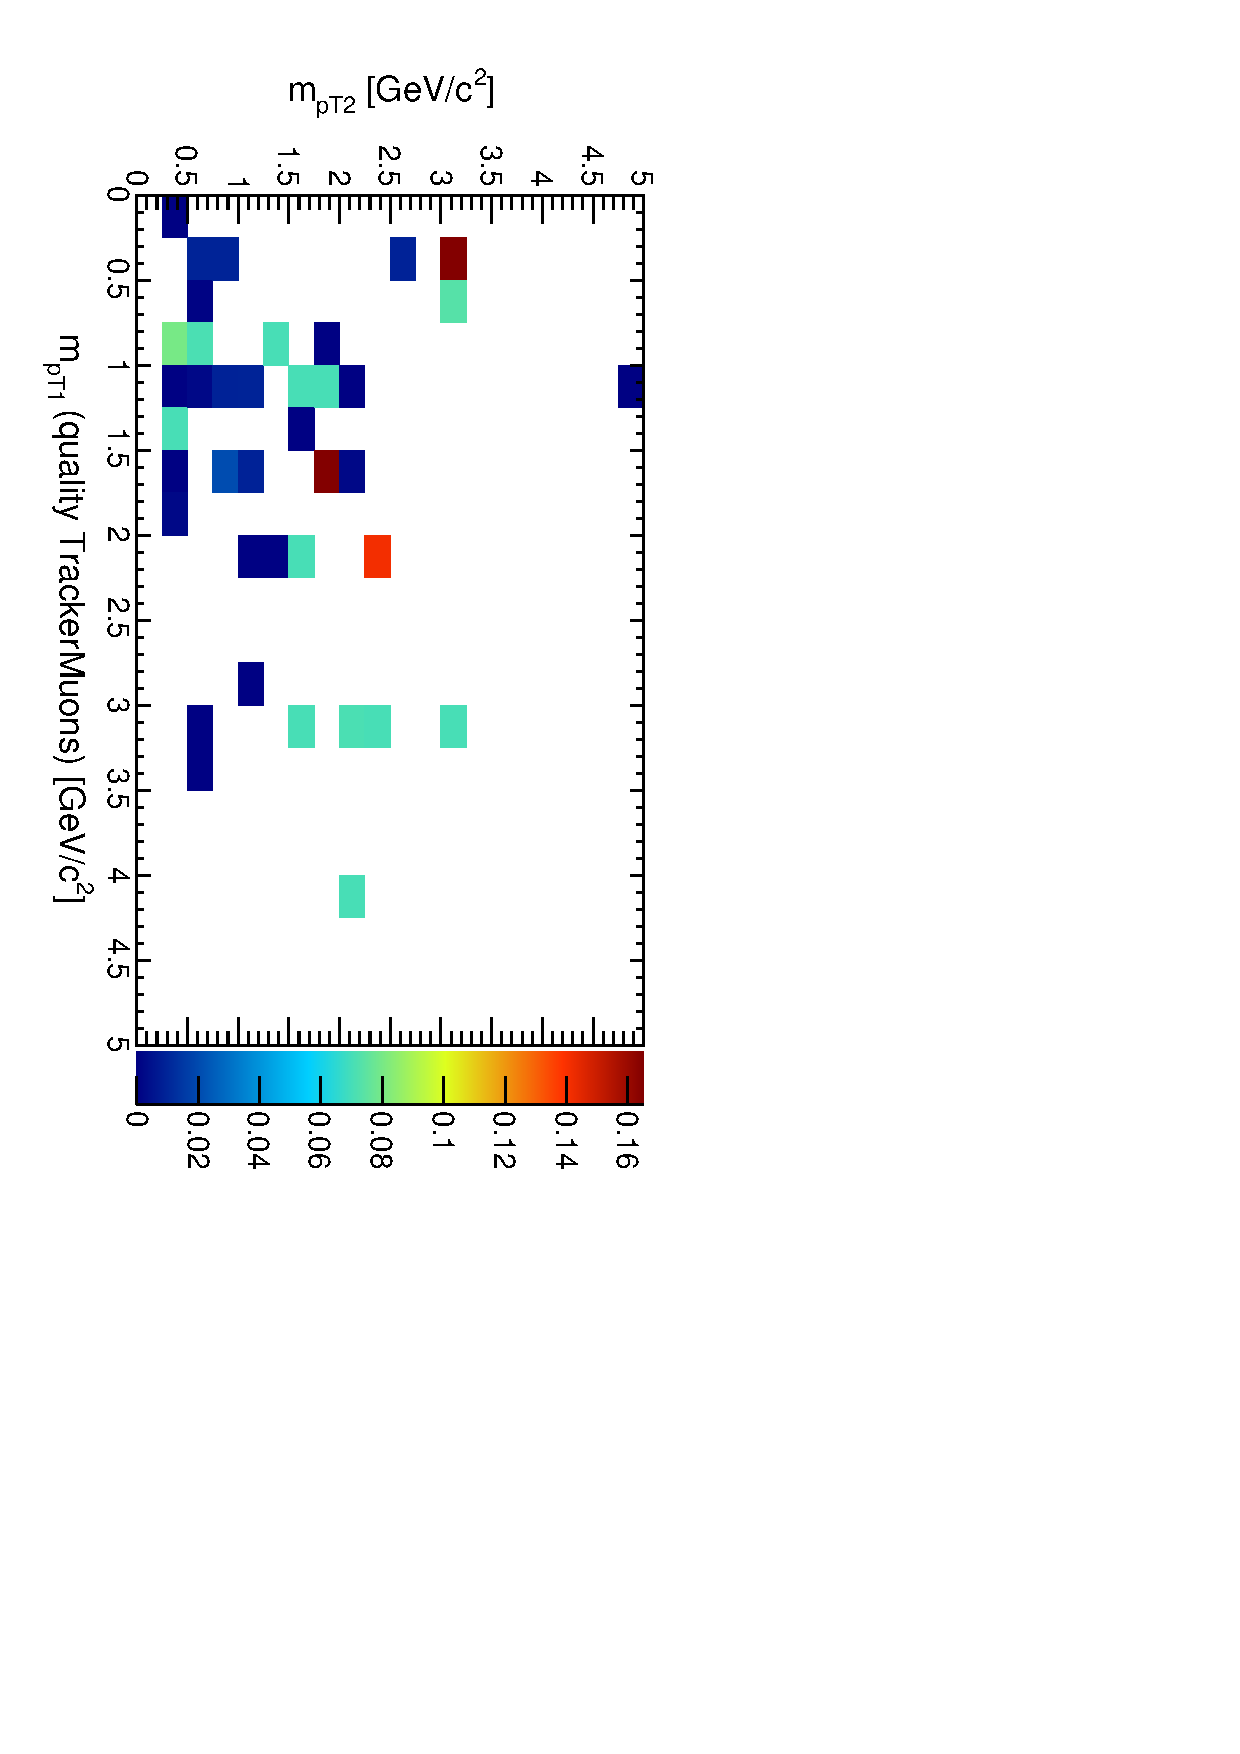
\includegraphics[width=4 cm, angle=90]{m12m34bypt_QualityTrackerMuonAny.pdf}
\end{frame}

\begin{frame}
\frametitle{Signals: mass peaks}

\begin{columns}
\column{0.5\linewidth}
Pair-pair $\mu$ gun with both pairs having the same mass

\includegraphics[height=\linewidth, angle=90]{m12m34.pdf}

\column{0.5\linewidth}
NMSSM Higgs with $h \to aa \to 4\mu$ ($m_h = 100$, $m_a = 2$~GeV/$c^2$)

\only<1>{\includegraphics[height=\linewidth, angle=90]{m12m34_bypt_NMSSM_pileup_QualityTrackerMuonAny.pdf}}
\only<2>{\includegraphics[height=\linewidth, angle=90]{m12m34_bypt_NMSSM_pileup_QualityTrackerMuonAny_lego.pdf}}
\end{columns}

\vspace{0.25 cm}
\begin{columns}
\column{0.5\linewidth}
Extra-$\mathcal{U}(1)$ dark matter model with $\gamma_\s{dark} \to
\mu^+\mu^-$, $m_\gamma = 1$~GeV/$c^2$

\only<1>{\includegraphics[height=\linewidth, angle=90]{m12m34_bypt_ExtraU1_pileup_QualityTrackerMuonAny.pdf}}
\only<2>{\includegraphics[height=\linewidth, angle=90]{m12m34_bypt_ExtraU1_pileup_QualityTrackerMuonAny_lego.pdf}}

\column{0.5\linewidth}
Same with $h_\s{dark} \to \gamma_\s{dark} \gamma_\s{dark}$, $m_\gamma
= 3$~GeV/$c^2$

\only<1>{\includegraphics[height=\linewidth, angle=90]{m12m34_bypt_ExtraU1higgs_pileup_QualityTrackerMuonAny.pdf}}
\only<2>{\includegraphics[height=\linewidth, angle=90]{m12m34_bypt_ExtraU1higgs_pileup_QualityTrackerMuonAny_lego.pdf}}
\end{columns}
\end{frame}

\begin{frame}
\frametitle{Isolation variables}

\begin{itemize}
\item If we were to apply the standard muon isolation, neighboring muons would cancel each other out
\item Redefined $\sum |p_T|$ and number-over-threshold isolation
  variables to exclude all muons in a muon group
\item Applying this isolation can further suppress QCD backgrounds by about a factor of 10 (100~pb$^{-1}$ analysis $\to$ 1~fb$^{-1}$ analysis)
\item QCD backgrounds (one $\mu$-group) on left, pair-gun signal with pileup on right (example signals are similar)
\end{itemize}

\includegraphics[height=0.5\linewidth, angle=90]{tkisolation_QualityTrackerMuonAny_backgrounds.pdf}
\includegraphics[height=0.5\linewidth, angle=90]{tkisolation_QualityTrackerMuonAny_PairGun100_pileup.pdf}
\end{frame}

\begin{frame}
\frametitle{Displaced vertices}

\begin{itemize}
\item Lepton Jets models require the new resonances to have weak couplings to Standard Model particles
\begin{itemize}
\item in extreme limit, they would be displaced from the \mbox{beamline ($v_{xy}$)\hspace{-1 cm}}
\end{itemize}
\item L1 trigger is sensitive to a wide range of $v_{xy}$, but HLT
  isn't because its StandAloneMuons are reconstructed with a beamline
  constraint
\item Track reconstruction is only sensitive up to about half of the
  tracker
\item Special 7-iteration tracking developed for $\gamma$ conversions-finding (green) doesn't help much (it was worth a try)
\end{itemize}

\begin{center}
\includegraphics[height=0.7\linewidth, angle=90]{dispvert.pdf}
\end{center}
\end{frame}

\begin{frame}
\frametitle{Displaced vertices}
\begin{itemize}
\item Quality cuts seem to be cutting both signal and background:
  something should possibly be loosened for the displaced-vertex case
\item Left: QCD background effective cross-section; right: \mbox{signal efficiency\hspace{-1 cm}}
\item Top: no quality cuts; bottom: with quality cuts
\item<2> GlobalMuons without quality cuts are sensitive at the level \mbox{of 1~pb/cm\hspace{-1 cm}}
\end{itemize}

\begin{center}
\only<1>{\includegraphics[height=0.45\linewidth, angle=90]{dispvert_PlainTrackerMuonAny.pdf}
\includegraphics[height=0.45\linewidth, angle=90]{dispvert_eff_PlainTrackerMuonAny.pdf}

\includegraphics[height=0.45\linewidth, angle=90]{dispvert_QualityTrackerMuonAny.pdf}
\includegraphics[height=0.45\linewidth, angle=90]{dispvert_eff_QualityTrackerMuonAny.pdf}}
\only<2>{\includegraphics[height=0.45\linewidth, angle=90]{dispvert_PlainGlobalMuonAny.pdf}
\includegraphics[height=0.45\linewidth, angle=90]{dispvert_eff_PlainGlobalMuonAny.pdf}

\includegraphics[height=0.45\linewidth, angle=90]{dispvert_QualityGlobalMuonAny.pdf}
\includegraphics[height=0.45\linewidth, angle=90]{dispvert_eff_QualityGlobalMuonAny.pdf}}
\end{center}
\end{frame}

%% \section*{First section}
%% \begin{frame}
%% \begin{center}
%% \Huge \textcolor{blue}{First section}
%% \end{center}
%% \end{frame}

\begin{frame}
\frametitle{Conclusions}
\begin{itemize}\setlength{\itemsep}{0.25 cm}
\item Physics results
\begin{itemize}
\item muon-grouping algorithm is now mature, guaranteed to find low-mass resonances, and safe against pile-up
\item StandAlone/GlobalMuon inefficiencies traced to overlapping segments in endcap, still not clear in the barrel
\item TrackerMuons are safe to use as long as we require $N_\s{segments} \ge 2$
\item understanding the exact trigger efficiency will be challenging
\item two $\mu$-group QCD backgrounds are 1~pb and $\sim$flat in mass
\item displaced vertex (``case (d)'') has not been fully optimized
\end{itemize}

\item Perspective
\begin{itemize}
\item it was important to develop $\mu$-group objects, because now they can be used as an analysis tool
\item we've laid the groundwork for a $\ge 2$ $\mu$-group analysis \\ (``case (b)'')
\end{itemize}
\end{itemize}
\label{numpages}
\end{frame}

\end{document}
